\chapter{Static Program Analysis}
\label{chap_static}
\targets{
  \item Understand the principles and the challenges of static analysis.
  \item Learn some techniques like: dataflow analysis,  analysis by abstract interpretation, deductive verification.
  \item Use tools for those techniques: Frama-C.
}

\section{Informal Introduction}

\begin{frame}{Static Program Analysis}
\begin{itemize}
  \item The previous verification technique was Testing.
  \item Testing and Runtime Verification require the execution of the software under verification: Dynamic analysis.
  \item Static analysis is a set of techniques used to study the behavior of programs by reasoning on their behavior without any execution.
  \item \textbf{Static program analysis} reason on the source code of the program, while the other static methods reason on models and specifications of the programs.
  \item Proving Properties about the code such as being free of a certain type of bugs.
  \item \textbf{Static analysis} is not perfect. 
\end{itemize}
\end{frame}

\begin{frame}[fragile]{Static Program Analysis}{Programming Paradigms}

Programs are written in programming languages:
\begin{itemize}
	\item Imperative Paradigm : C, C++, Java, Scala, Rust \dots
	\item Functional Paradigm : Haskell, OCaml, Lisp, Scala \dots
\end{itemize}

\tiny
\begin{columns}
		\column{0.44\linewidth}
		\centering
	\begin{lstlisting}[language=Scala,caption={Scala Imperative}]
     def sort(xs: Array[Int]) {
      def swap(i: Int, j: Int) {
       val t = xs(i);
       xs(i) = xs(j);
       xs(j) = t;} 
      
     def sort1(l: Int, r: Int) {
      val pivot = xs((l + r) / 2)
      var i = l; var j = r
      while (i <= j) {
      while (xs(i) < pivot) i += 1
      while (xs(j) > pivot) j -= 1
      if (i <= j) {
      swap(i, j)
      i += 1
      j -= 1} }
     if (l < j) sort1(l, j)
     if (j < r) sort1(i, r) }
     sort1(0, xs.length - 1)} 
    \end{lstlisting}
    
   	\column{0.50\linewidth}
    \centering
   \tiny 

	\begin{lstlisting}[language=Scala,caption={Scala Functionnal}]

  def sort(xs: Array[Int]): Array[Int] 
  = {
   if (xs.length <= 1) xs
   else {
   val pivot = xs(xs.length / 2)
   Array.concat(
   sort(xs filter (pivot >)),
   xs filter (pivot ==),
   sort(xs filter (pivot <)))
  }}
    \end{lstlisting}
\end{columns}

\end{frame}

\begin{frame}{Static Analysis}{Since the early ages of programming}
\begin{itemize}
\item Compilers (fully automated, bugs elimination and optimization).
\item Code review (informal, incomplete).
\item Formal methods (logical proofs, hard and sometimes undecidable).
\end{itemize}

\end{frame}


\begin{frame}{Static Analysis}{Compiler Level}
\begin{enumerate}
\item When you have a compiling error, ehe error was established by a static analysis:
\begin{itemize}
	\item Type Checking.
	\item Syntax Checking. 
	\item non declared variables, functions, ...
\end{itemize}
\centering 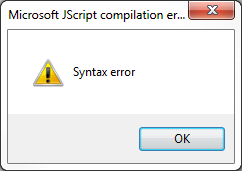
\includegraphics[scale=0.50]{content/images/static-analysis/syntaxerr.png}
\item But compilers use static analysis for optimization as well.
\end{enumerate}
\end{frame}

\begin{frame}{Static Program Analysis}{Compiler Optimization}
Example: Detection and removal of unnecessary variables.
	\centering
	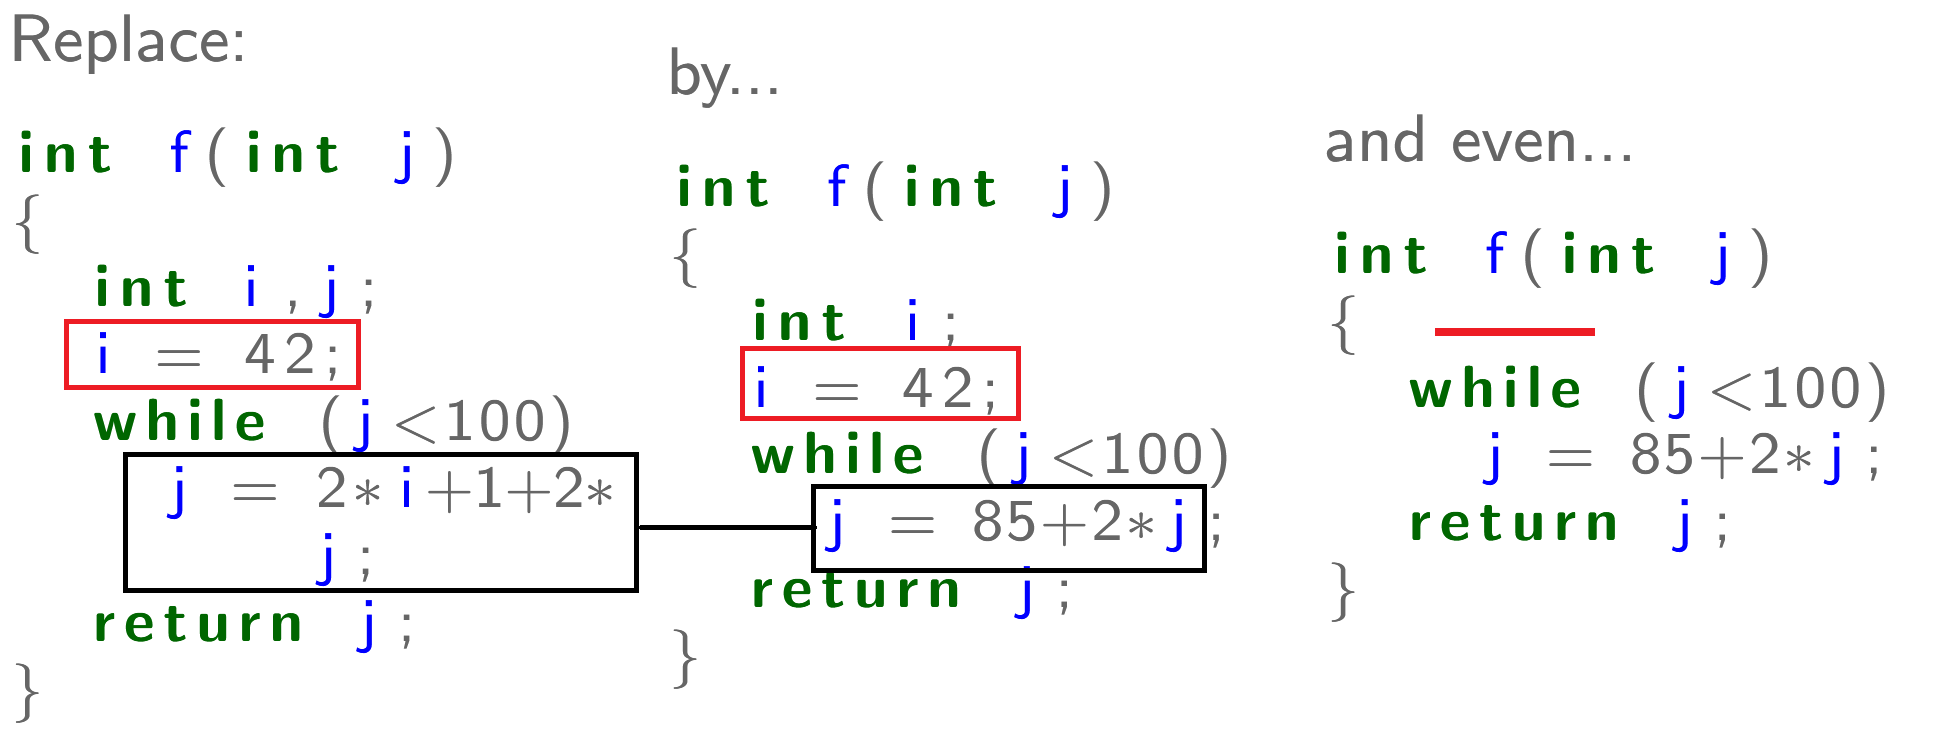
\includegraphics[scale=0.37]{content/images/static-analysis/compiler.png}

\end{frame}



\begin{frame}{Static Analysis}{Code Review}
\begin{columns}
	\column{0.58\linewidth}
\begin{itemize}
	\item Performed by expert programmers.
	\item Finding bugs without Testing.
	\item Quantifying the quality of the coding style.
	\item Rare talents ...
\end{itemize}
\column{0.38\linewidth}
\centering
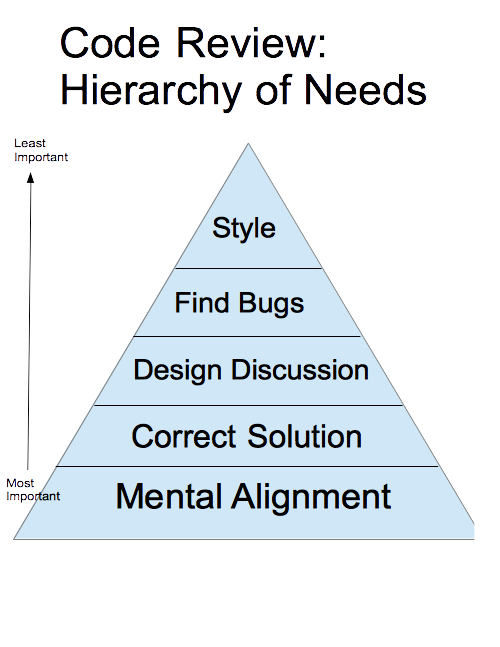
\includegraphics[scale=0.3]{content/images/static-analysis/review.png}
\end{columns}
\end{frame}


\begin{frame}{Static Analysis}{Code Review}
	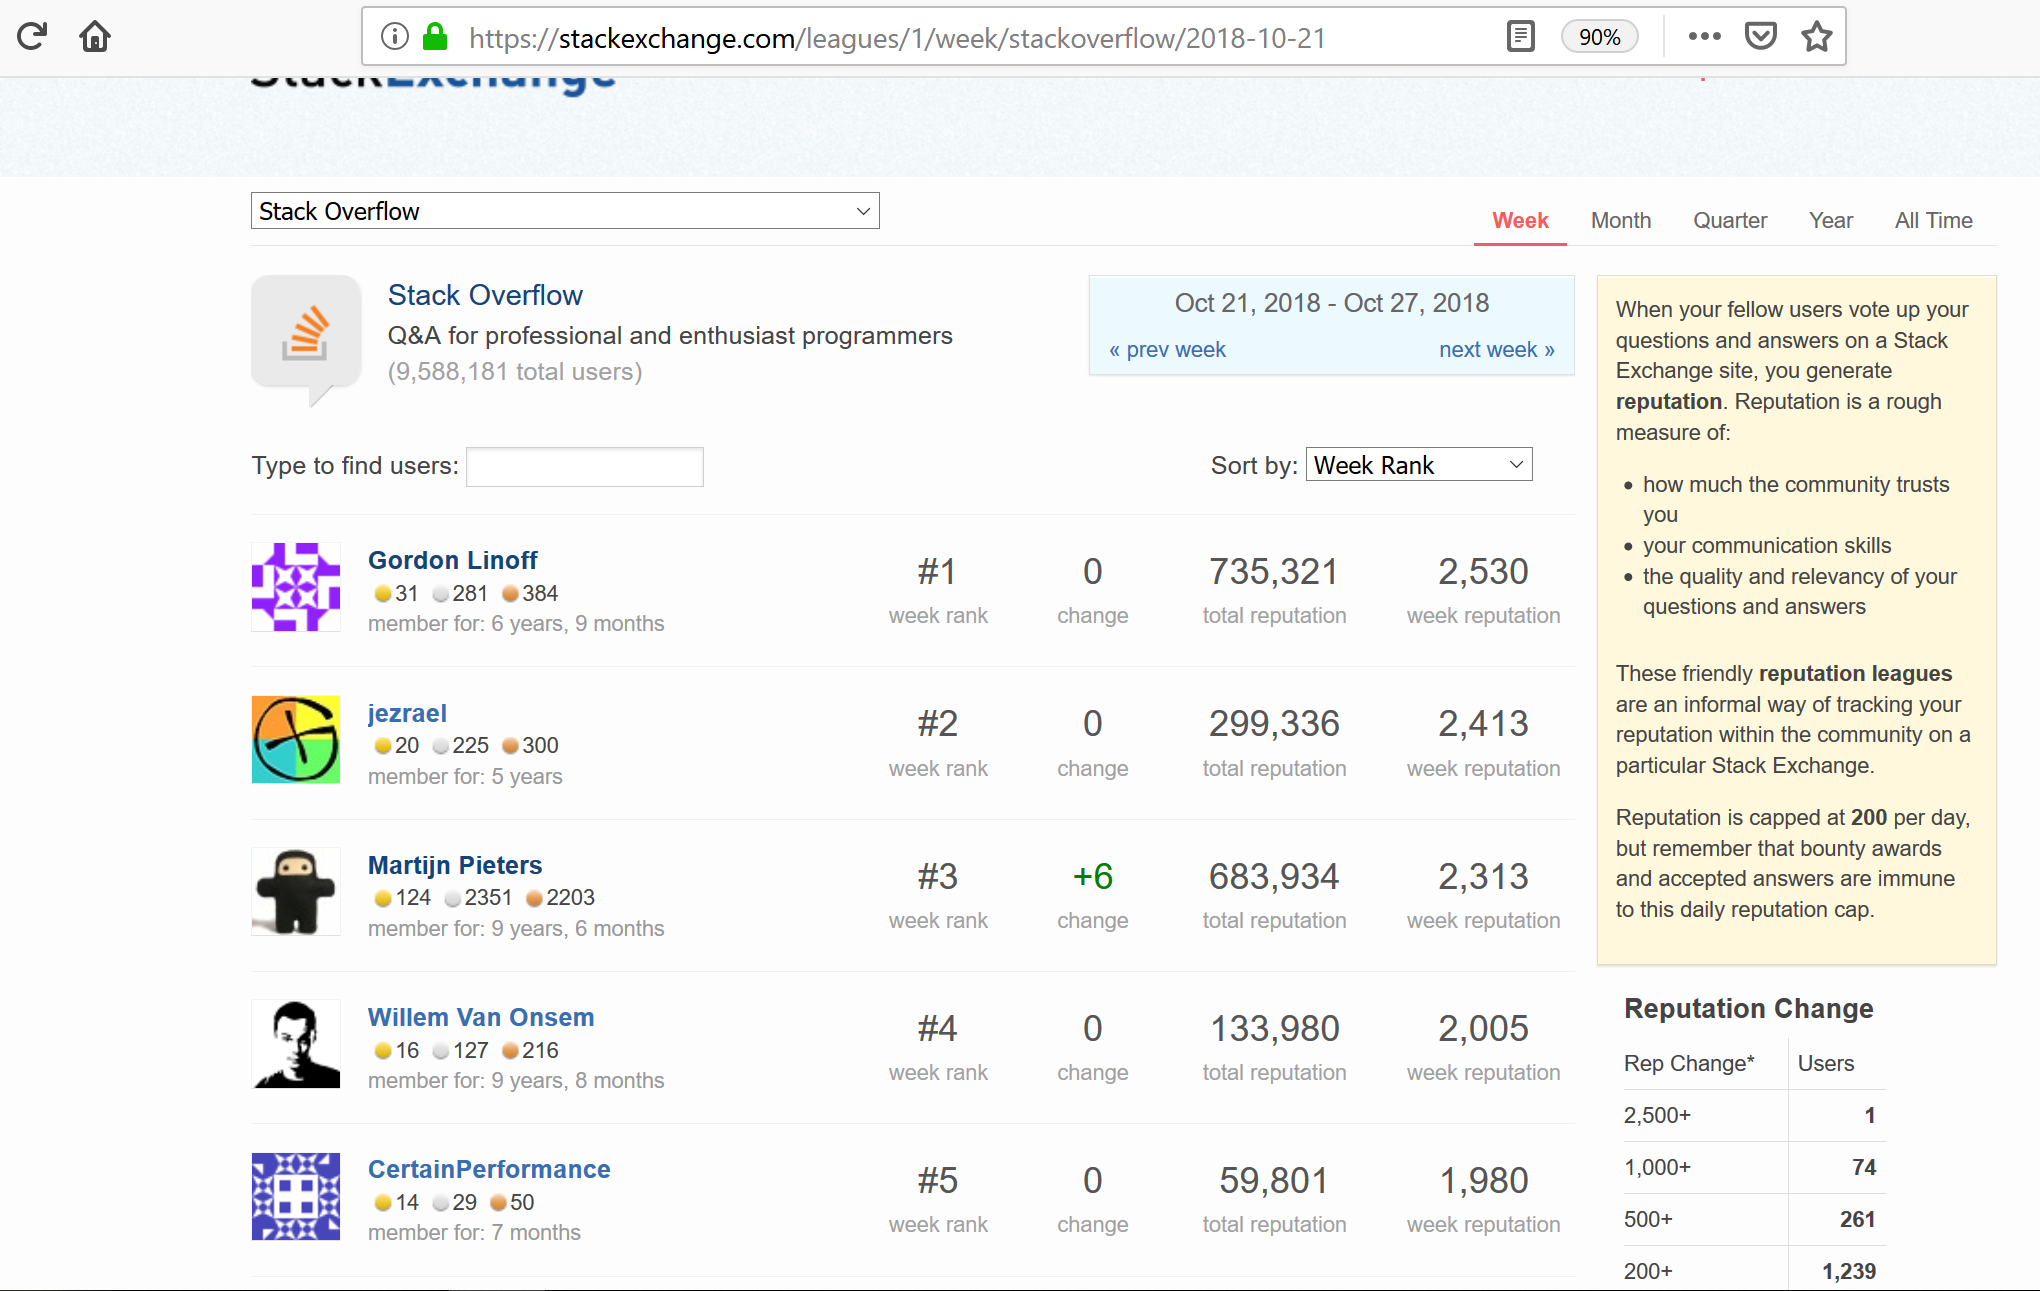
\includegraphics[scale=0.35]{content/images/static-analysis/Static.png}
\end{frame}


\begin{frame}{Static Analysis}{Formal Methods}
A \textbf{formal method} is built on top of mathematical and logical foundations such as:
\begin{itemize}
	\item Type Theory. (strongly typed)
	\item Symbolic Execution.
	\item (Data/Control) Flow Analysis.
	\item Analysis by Abstract interpretation.
	\item Deductive program verification. 
\end{itemize}
\end{frame}


\section{Challenges}
\begin{frame}{Challenges}
\begin{itemize}
	\item Undecidability. 
	\item Soundness, completeness, precision.
	\item Building tools: automation and usability.
\end{itemize}
\end{frame}

\begin{frame}
\frametitle{Undecidability}
\textit{"All \textbf{interesting properties} of the behavior of programs written in common programming languages are mathematically undecidable.}"  From Rice's Theorem [1953].
\newline

\textbf{Interesting properties} are:
\begin{itemize}
	\item Semantic properties: About the program's Behavior $\neq$ Syntactic properties.
	\item Non-trivial properties: For which depending on the input the answer is not always true and not always false.
\end{itemize} 

\end{frame}


\begin{frame}
\frametitle{Complexity: Undecidability}


Rice's theorem was Proposed in 1953
\begin{itemize}
	\item Undecidability of termination was proven by Alan Turing in 1936.
	\item Proofs of undecidability are done by reduction :\\
	if $Prob_x$ is undecidable, if $Prob_y \mapsto Prob_x$ then  $Prob_y$ is undecidable.
	
\end{itemize}
\xxx
\footnotesize
\begin{tabular}{|c|c|}
	\hline
	Syntactic & Semantic\\
	\hline 
	$P$ has n statements &  $P$ terminates\\
	
	$P_1 =_{syn} P_2$  & $\forall x.P_1(x) = P_2(x)$\\
	$P$ contains n program functions &  $P \equiv f$ ($f$ a mathematical function)\\
	\hline
\end{tabular}

\end{frame}

\begin{frame}
\frametitle{Complexity: Undecidability}
\textit{"All interesting properties of the behavior of programs written in common programming languages are mathematically \textbf{undecidable}."} From Rice's Theorem [1953]
\newline

\textbf{Undecidable:}
\begin{itemize}
	\item There is no general algorithm that can always decide for all classes of programs if the property is either verified or not. 
	\item \textbf{Solutions}: 
	\begin{enumerate}
		\item Identify a subclass of programs for which the verification problem is decidable.
		\item Approximate (Partial correctness, weaker properties). 
		\item Use dynamic methods to complement.
	\end{enumerate}
\end{itemize} 
\end{frame}


\begin{frame}{Soundness and Completeness}
Tools rely on algorithms to detect "errors", for a verification algorithm:
\begin{itemize}
	\item \textcolor{blue}{Completeness}:\newline Run of the algorithm claims finding a bug $B$ $\Rightarrow$ $B$ is a real bug for the program.
	\textbf{(No false positive)}
	\item \textcolor{blue}{Soundness}:\newline The software contains a bug $\Rightarrow$  Run of the algorithm will detect it. \textbf{(No false negative)}
\end{itemize}
\centering
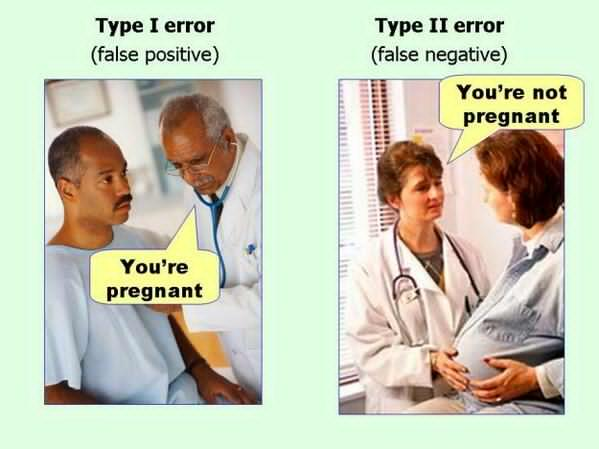
\includegraphics[scale=0.30]{content/images/static-analysis/FpFN.jpg}
\end{frame}


\begin{frame}{Soundness and Completeness}
Tools rely on algorithms to detect "errors":
\begin{itemize}
	\item \textbf{Completeness}:\newline Run of the algorithm finds an error $\Rightarrow$ The error is a real bug of the program.
	 \textbf{(No false positive)}
	\item \textbf{Soundness}:\newline The software contains a bug $\Rightarrow$  Run of the algorithm will Detect it.\textbf{(No false negative)}
	\item A \textbf{correct} algorithm ensures both soundness, completeness and  \textbf{terminates}. 
	\item In practice, completeness can be sacrificed but losing soundness is not desired for safety critical systems. Termination is a must have.
\end{itemize}
\end{frame}

\begin{frame}{Static Program Analysis}{Building Tools}
\centering 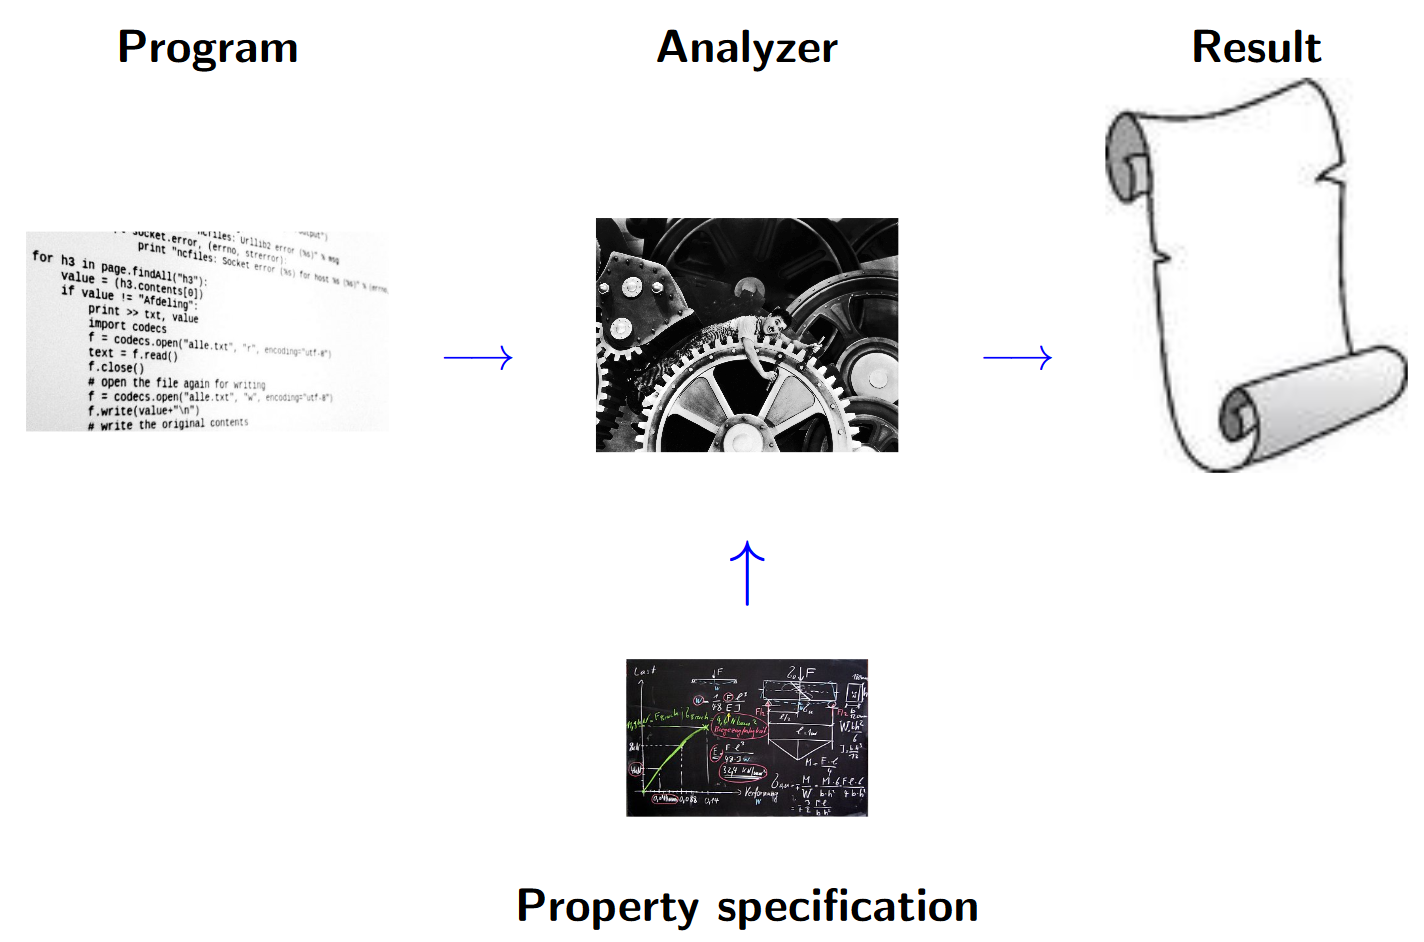
\includegraphics[scale=0.50]{content/images/static-analysis/tool.png}
\end{frame}



\begin{frame}{Static Program Analysis}{Building Tools}
\begin{itemize}
	\item \textbf{Deal/solve} with/the theoretical limitations and complexity.
	\item \textbf{Automation}: Implementing algorithms, using solvers for proofs (SMT), \dots
	\item \textbf{Usability}: Scalability, performance, fully to semi-automatic \dots
	\item Static software analyzers are \textbf{software} as well: 
	\begin{enumerate}
		\item May contain bugs. How to certify Static Analysis tools?
		\item Developed by a team and has to be maintained.
	\end{enumerate} 
\end{itemize}
\end{frame}


\section{Syntax of a mini-imperative language}
\begin{frame}{The mini-imperative language: Syntax of expressions}
\centering
\lstinputlisting[escapeinside=`',basicstyle=\footnotesize]{content/images/static-analysis/syntaxexp.tex}

\end{frame}

\begin{frame}{The mini-imperative language: Syntax of Statements}
\centering
\lstinputlisting[escapeinside=`',basicstyle=\footnotesize]{content/images/static-analysis/syntaxstat.tex}

\end{frame}

\section{Flow Analysis}
\begin{frame}{Control Flow Analysis}
\begin{itemize}
\item Control flow analysis is a way to understand the control structure of a program.

\item Can Be:
\begin{enumerate}
\item Intra-procedural: if the program is made out of one function.	
\item Inter-procedural: if the program is made out of multiple functions depending on each other. (out of the scope of this course)	
\end{enumerate}
\end{itemize}
\end{frame}


\begin{frame}{Control Flow Analysis: Inter-procedural}
\textbf{Inter-procedural analysis}: We need to understand how the execution of the multi-functions program is done:
\begin{itemize}
	\item What are the functions that were executed.
	\item In which order are the used functions are called.
	\item How many times was a function executed?
	\item Modeling by a \textbf{callgraph}.
\end{itemize}
\end{frame}

\begin{frame}{Control Flow Analysis: Inter-procedural}
\begin{exampleblock}{Example of a callgraph}
\begin{columns}
	\column{0.60\linewidth}
	\lstinputlisting[language=C, basicstyle =\tiny]{content/images/static-analysis/callgraph.c}

\column{0.32\linewidth}
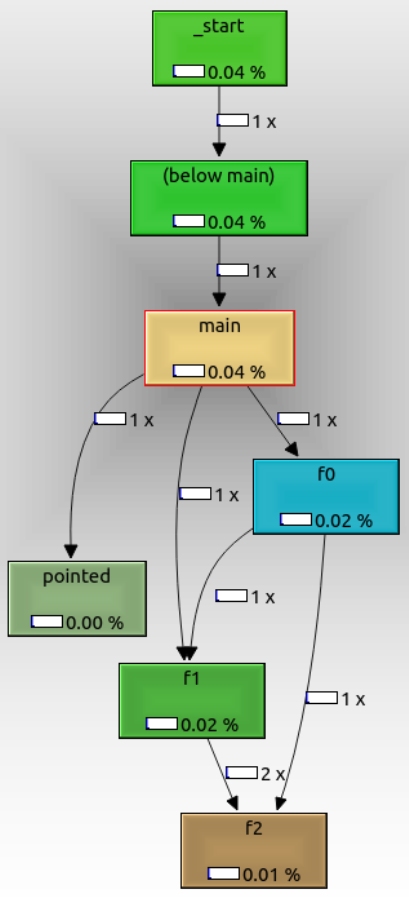
\includegraphics[scale=0.55]{content/images/static-analysis/callgraph.png}
\end{columns}
\end{exampleblock}
\end{frame}


\begin{frame}{Control Flow Analysis: Intra-procedural}
\textbf{Intra-procedural analysis}: We need to understand how the execution of a succession of statements is done:
\begin{itemize}
	\item Are all the program statements executed? (dead code)
	\item How many times a statement is going to be executed?
	\item We construct a \textbf{control flow graph. (CFG)}
	\item Pretty easy to construct a CFG for programs written in imperative languages.

\end{itemize}
\end{frame}

\begin{frame}{Control Flow Analysis: Intra-procedural}
\begin{exampleblock}{Example of Control Flow diagram}
\begin{columns}
	\column{0.4\linewidth}
	\lstinputlisting[language=C, basicstyle =\scriptsize]{content/images/static-analysis/CFG.c}
	
	\column{0.6\linewidth}
	

  \tiny
  \begin{tikzpicture}[%
    ->,
    shorten >=2pt,
    >=stealth,
    node distance=0.7cm,
    noname/.style={%
      rectangle,
      minimum width=5em,
      minimum height=3em,
      draw
    }
  ]
    \node[noname] (1)                                             {[ y = 2;] $l_1$};
    \node[noname] (2) [below=of 1]                                {[ x = y + 1;] $l_2$};
    \node[noname] (3) [below=of 2]                                {[ if ( x == 4) ] $l_3$};
    \node[noname] (4) [below right=of 3]                          {[ y = 6;] $l_4$};
    \node[noname] (5) [below= 1.5cm of 3]                         {[ while (x <1000) ] $l_5$};
    \node[noname] (6) [below right=of 5]                          {[ x = x + 1;] $l_6$};
    \node[noname] (7) [below=of 5]                                {[ y = x - 3;] $l_7$};

    \path (1) edge                   node {} (2)
          (2) edge                   node {} (3)
          (3) edge                   node [yshift=5pt,right]{yes} (4)
          (4) edge                   node {} (5)
          (3) edge                   node [yshift=5pt,right]{no} (5)
          (5) edge [bend right=20pt] node [yshift=3pt,right]{yes} (6)
          (5) edge                   node [yshift=5pt,right]{no} (7)
          (6) edge [bend right=20pt] node {} (5);
  \end{tikzpicture}
\end{columns}
\end{exampleblock}
\end{frame}


\begin{frame}{Control Flow Analysis: Intra-procedural}
\begin{exampleblock}{Example of Control Flow diagram}
	\begin{columns}
		\column{0.4\linewidth}
		\footnotesize
		\begin{itemize}
		\item Is the program always going to run that way ?
	    \item Is both branches of the 'if' statement going to be taken? (at $l_3$)
		\end{itemize}
		\column{0.6\linewidth}
		

  \tiny
  \begin{tikzpicture}[%
    ->,
    shorten >=2pt,
    >=stealth,
    node distance=0.7cm,
    noname/.style={%
      rectangle,
      minimum width=5em,
      minimum height=3em,
      draw
    }
  ]
    \node[noname] (1)                                             {[ y = 2;] $l_1$};
    \node[noname] (2) [below=of 1]                                {[ x = y + 1;] $l_2$};
    \node[noname] (3) [below=of 2]                                {[ if ( x == 4) ] $l_3$};
    \node[noname] (4) [below right=of 3]                          {[ y = 6;] $l_4$};
    \node[noname] (5) [below= 1.5cm of 3]                         {[ while (x <1000) ] $l_5$};
    \node[noname] (6) [below right=of 5]                          {[ x = x + 1;] $l_6$};
    \node[noname] (7) [below=of 5]                                {[ y = x - 3;] $l_7$};

    \path (1) edge                   node {} (2)
          (2) edge                   node {} (3)
          (3) edge                   node [yshift=5pt,right]{yes} (4)
          (4) edge                   node {} (5)
          (3) edge                   node [yshift=5pt,right]{no} (5)
          (5) edge [bend right=20pt] node [yshift=3pt,right]{yes} (6)
          (5) edge                   node [yshift=5pt,right]{no} (7)
          (6) edge [bend right=20pt] node {} (5);
  \end{tikzpicture}
	\end{columns}
\end{exampleblock}
\end{frame}


\begin{frame}{Control Flow Analysis: Intra-procedural}
\begin{exampleblock}{Example of Control Flow diagram}
	\begin{columns}
		\column{0.4\linewidth}
		\footnotesize
		\begin{itemize}
			\item The yes branch is dead.
			\item The nodes $l_3$ and $l_4$ are useless. (If statement can be removed).
		\end{itemize}
		
		\column{0.6\linewidth}
		

  \tiny
  \usetikzlibrary{trees,shapes,decorations}
  \begin{tikzpicture}[%
    ->,
    shorten >=2pt,
    >=stealth,
    node distance=0.7cm,
    noname/.style={%
      rectangle,
      minimum width=5em,
      minimum height=3em,
      draw
    }
  ]
    \node[noname] (1)                                             {[ y = 2;] $l_1$};
    \node[noname] (2) [below=of 1]                                {[ x = y + 1;] $l_2$};
    \node[noname] (3) [below=of 2]                                {[ if ( x == 4) ] $l_3$};
    
    \node[ellipse,
    minimum width=5em,
    minimum height=2em,draw] (12) [right= of 2] {x value is 3};
    
    \node[ellipse,
    minimum width=5em,
    minimum height=2em,draw] (13) [right= of 3] {if returns no};
    
    \node[rectangle,
    minimum width=5em,
    minimum height=2em,draw] (4) [below right=of 3]                          {\color{white} [ y = 6;] $l_4$};
     {};
     
     \node[
     minimum width=5em,
     minimum height=2em,cross out,color=red,draw] (11) [fill=green!30!black!70,below right=of 3]   {[ y = 6;] $l_4$};      
 
    \node[noname] (5) [below= 1.5cm of 3]                         {[ while (x <1000) ] $l_5$};
    \node[noname] (6) [below right=of 5]                          {[ x = x + 1;] $l_6$};
    \node[noname] (7) [below=of 5]                                {[ y = x - 3;] $l_7$};

    \path (1) edge                   node {} (2)
          (2) edge                   node {} (3)
          (3) edge                   node [yshift=5pt,right,color=red]{yes} (4)
          (4) edge                   node {} (5)
          (3) edge                   node [yshift=5pt,right]{no} (5)
          (5) edge [bend right=20pt] node [yshift=3pt,right]{yes} (6)
          (5) edge                   node [yshift=5pt,right]{no} (7)
          (6) edge [bend right=20pt] node {} (5);
  \end{tikzpicture}
	\end{columns}
\end{exampleblock}
\end{frame}

\begin{frame}{Control Flow Analysis: Intra-procedural}
\begin{exampleblock}{Example of Control Flow diagram}
	\begin{columns}
		\column{0.4\linewidth}
		\footnotesize
			\begin{itemize}
			\item The nodes $l_3$ and $l_4$ are useless. (both statements can be removed).
			\item How about the branches of $l_5$? (While statement)
		\end{itemize}
		
		\column{0.6\linewidth}
		

  \tiny
  \usetikzlibrary{trees,shapes,decorations}
  \begin{tikzpicture}[%
    ->,
    shorten >=2pt,
    >=stealth,
    node distance=0.7cm,
    noname/.style={%
      rectangle,
      minimum width=5em,
      minimum height=3em,
      draw
    }
  ]
    \node[noname] (1)                                             {[ y = 2;] $l_1$};
    \node[noname] (2) [below=of 1]                                {[ x = y + 1;] $l_2$};
    \node[noname] (3) [below=of 2]                                {[ if ( x == 4) ] $l_3$};
    
    \node[ellipse,
    minimum width=5em,
    minimum height=2em,draw] (12) [right= of 2] {x value is 3};
    
    \node[ellipse,
    minimum width=5em,
    minimum height=2em,draw] (13) [right= of 3] {if returns no};
    
    \node[rectangle,
    minimum width=5em,
    minimum height=2em,draw] (4) [below right=of 3]                          {\color{white} [ y = 6;] $l_4$};
     {};
     
     \node[
     minimum width=5em,
     minimum height=2em,cross out,color=red,draw] (11) [fill=green!30!black!70,below right=of 3]   {[ y = 6;] $l_4$};      
 
    \node[noname] (5) [below= 1.5cm of 3]                         {[ while (x <1000) ] $l_5$};
    \node[noname] (6) [below right=of 5]                          {[ x = x + 1;] $l_6$};
    \node[noname] (7) [below=of 5]                                {[ y = x - 3;] $l_7$};

    \path (1) edge                   node {} (2)
          (2) edge                   node {} (3)
          (3) edge                   node [yshift=5pt,right,color=red]{yes} (4)
          (4) edge                   node {} (5)
          (3) edge                   node [yshift=5pt,right]{no} (5)
          (5) edge [bend right=20pt] node [yshift=3pt,right]{yes} (6)
          (5) edge                   node [yshift=5pt,right]{no} (7)
          (6) edge [bend right=20pt] node {} (5);
  \end{tikzpicture}
	\end{columns}
\end{exampleblock}
\end{frame}



\begin{frame}{Control Flow Analysis: Intra-procedural}
\begin{exampleblock}{Example of Control Flow diagram}
	\begin{columns}
		\column{0.4\linewidth}
		\footnotesize
		\begin{itemize}
			\item How about the branches of $l_5$? (While statement)
			\item We have to keep calculating the value of $x$ in order to evaluate $(x<1000)$
			\item This is called \textbf{constant propagation}.
		\end{itemize}
		
		\column{0.6\linewidth}
		

  \tiny
  \usetikzlibrary{trees,shapes,decorations}
  \begin{tikzpicture}[%
    ->,
    shorten >=2pt,
    >=stealth,
    node distance=0.7cm,
    noname/.style={%
      rectangle,
      minimum width=5em,
      minimum height=3em,
      draw
    }
  ]
    \node[noname] (1)                                             {[ y = 2;] $l_1$};
    \node[noname] (2) [below=of 1]                                {[ x = y + 1;] $l_2$};
    \node[noname] (3) [below=of 2]                                {[ if ( x == 4) ] $l_3$};
    
    \node[ellipse,
    minimum width=5em,
    minimum height=2em,draw] (12) [right= of 2] {x value is 3};
    
    \node[ellipse,
    minimum width=5em,
    minimum height=2em,draw] (13) [right= of 3] {if returns no};
    
    \node[rectangle,
    minimum width=5em,
    minimum height=2em,draw] (4) [below right=of 3]                          {\color{white} [ y = 6;] $l_4$};
     {};
     
     \node[
     minimum width=5em,
     minimum height=2em,cross out,color=red,draw] (11) [fill=green!30!black!70,below right=of 3]   {[ y = 6;] $l_4$};      
 
    \node[noname] (5) [below= 1.5cm of 3]                         {[ while (x <1000) ] $l_5$};
    \node[noname] (6) [below right=of 5]                          {[ x = x + 1;] $l_6$};
    \node[noname] (7) [below=of 5]                                {[ y = x - 3;] $l_7$};

    \path (1) edge                   node {} (2)
          (2) edge                   node {} (3)
          (3) edge                   node [yshift=5pt,right,color=red]{yes} (4)
          (4) edge                   node {} (5)
          (3) edge                   node [yshift=5pt,right]{no} (5)
          (5) edge [bend right=20pt] node [yshift=3pt,right]{yes} (6)
          (5) edge                   node [yshift=5pt,right]{no} (7)
          (6) edge [bend right=20pt] node {} (5);
  \end{tikzpicture}
	\end{columns}
\end{exampleblock}
\end{frame}

\begin{frame}{Control Flow Analysis}
\begin{itemize}
	\item Control flow analysis is about understanding how statements and block of statements will interact during the execution of the program.\\
	\item Can be refined by studying the Boolean statements in the conditionals and loops.
	\item Data flow analysis for control flow analysis.
	\item Does not really help to proof properties nor correctness of programs.
	\item For example: Path coverage is undecidable.
	
\end{itemize}
\end{frame}





\begin{frame}{Data Flow Analysis}
\begin{beameritemize}
	\item Static Analysis used to reason about the possible data computed at the different point of a program.
	\item Usage:
	 \begin{beameritemize}
		\item Live variables.
		\item Constant propagation. (Does the program compute bad values??)
		\item Available expressions.
	\end{beameritemize}
\end{beameritemize}
\end{frame}

%%%%%%%%%%%%%%%%%%%%%%%%%%%%%%%%%%%%%%%%%%%%%%
\begin{frame}{Data Flow Analysis}{Frameworks for Data Flow Analysis}
Depending on the properties we are interested in, we must define a \textbf{logical environment} for studying one property:
\begin{itemize}
	\item Define the informations to gather: \textbf{Domain of value $\mathbb{V}$} 
	\item Define a way to collect the semantics relevant to $\mathbb{V}$:
	\begin{itemize}
		\item \textbf{Transfer functions} over the set of statement labels: \textbf{ $F_L$}
		\item \textbf{Join operator} : \textbf{$\sqcup$}
	\end{itemize}
	\item Procedure for iterating over the program statements. (MFP or MOP)
	\item Iteration can be \textbf{backward} or \textbf{forward}.
	\item Depending on the algorithm (transfer function + iteration procedure ), get different results for the same program (precision).
\end{itemize}
\end{frame}
%%%%%%%%%%%%%%%%%%%%%%%%%%%%%%%%%%%%%%%%%%%%%%


\begin{frame}{Data Flow Analysis}{Informal Example}
\begin{exampleblock}{Live Variable: LV}
	\begin{columns}
		\column{0.52\linewidth}
		\begin{itemize}
			\item LV analysis define if for all variable there value is available for the program execution
			\item Proceed backwards.
		\end{itemize}
	
		\column{0.48\linewidth}
		\lstinputlisting[language=C, basicstyle =\scriptsize]{content/images/static-analysis/livevariables.c}
	\end{columns}	
	\end{exampleblock}
\end{frame}

\begin{frame}{Data Flow Analysis}{Informal Example}
\begin{exampleblock}{Live Variable: LV}
	\begin{columns}
		\column{0.45\linewidth}
		\begin{itemize}
			\small
			\item LV analysis define if for every variables there value is available for the program execution
			\item Proceed Backward.
		\end{itemize}
		
		\column{0.55\linewidth}
		  \tiny
  \usetikzlibrary{trees,shapes,decorations}
  \begin{tikzpicture}[%
    ->,
    shorten >=2pt,
    >=stealth,
    node distance=0.3cm,
    noname/.style={%
      rectangle,
      minimum width=5em,
      minimum height=2em,
      draw
    }
  ]
    \node[noname] (1)                                             {[ z = 1 ] $l_1$};
    \node[noname] (2) [below=of 1]                                {[ y = 2 ] $l_2$};
    \node[noname] (3) [below=of 2]                                {[ x = 3 ] $l_3$};
    \node[noname] (4) [below=of 3]                                {[ if (z > 0) ] $l_4$};
    \node[noname] (5) [below right=of 4]                          {[ y = z ] $l_5$};
    \node[noname] (6) [below=of 5]                                {[ if ( z < 2) ] $l_6$};
    \node[noname] (7) [below right=of 6]                                {[ z = 7 ] $l_7$};
    
%    \node[rectangle,
%    minimum width=5em,
%    minimum height=2em,draw] (9) [below= 2.5cm of 4] {\color{white}[ return y] $l_8$};
    \node[
    minimum width=5em,
    minimum height=2em,draw] (8) [fill=blue!80!black!20,below= 2.5cm of 4]                                {\color{black}[ return y] $l_8$};
    

      \path 
   (1) edge                   node {} (2)
   (2) edge                   node {} (3)
   (3) edge                   node {} (4)
   (4) edge                   node {} (5)
   (4) edge                   node [yshift=-25pt,right]{} (8)
   (5) edge                   node {} (6)
   (6) edge                   node {} (7)
   (7) edge                   node [above]{} (8)
   (6) edge                   node [above]{} (8);
 
          
  \end{tikzpicture}
\end{columns}	
\end{exampleblock}
\end{frame}

\begin{frame}{Data Flow Analysis}{Informal Example}
\begin{exampleblock}{Live Variable: LV}
	\begin{columns}
		\column{0.45\linewidth}
		\begin{itemize}
			\small
			\item We need the value of $y$ defined before returning its value. 
		\end{itemize}
		
		\column{0.55\linewidth}
		  \tiny
  \usetikzlibrary{trees,shapes,decorations}
  \begin{tikzpicture}[%
    ->,
    shorten >=2pt,
    >=stealth,
    node distance=0.3cm,
    noname/.style={%
      rectangle,
      minimum width=5em,
      minimum height=2em,
      draw
    }
  ]
    \node[noname] (1)                                             {[ z = 1 ] $l_1$};
    \node[noname] (2) [below=of 1]                                {[ y = 2 ] $l_2$};
    \node[noname] (3) [below=of 2]                                {[ x = 3 ] $l_3$};
    \node[noname] (4) [below=of 3]                                {[ if (z > 0) ] $l_4$};
    \node[noname] (5) [below right=of 4]                          {[ y = z ] $l_5$};
    \node[noname] (6) [below=of 5]                                {[ if ( z < 2) ] $l_6$};
    \node[noname] (7) [below right=of 6]                                {[ z = 7 ] $l_7$};
    
%    \node[rectangle,
%    minimum width=5em,
%    minimum height=2em,draw] (9) [below= 2.5cm of 4] {\color{white}[ return y] $l_8$};
    \node[
    minimum width=5em,
    minimum height=2em,draw] (8) [fill=blue!80!black!20,below= 2.5cm of 4]                                {\color{black}[ return y] $l_8$};
    

      \path 
   (1) edge                   node {} (2)
   (2) edge                   node {} (3)
   (3) edge                   node {} (4)
   (4) edge                   node {} (5)
   (4) edge                   node [yshift=-25pt,right]{\{y\}} (8)
   (5) edge                   node {} (6)
   (6) edge                   node {} (7)
   (7) edge                   node [above]{\{y\}} (8)
   (6) edge                   node [above]{\{y\}} (8);
 
          
  \end{tikzpicture}
	\end{columns}	
\end{exampleblock}
\end{frame}


\begin{frame}{Data Flow Analysis}{Informal Example}
\begin{exampleblock}{Live Variable: LV}
	\begin{columns}
		\column{0.45\linewidth}
		\begin{itemize}
			\small
			\item The value of $z$ is defined in this instruction, no need to track it. 
		\end{itemize}
		
		\column{0.55\linewidth}
		  \tiny
  \usetikzlibrary{trees,shapes,decorations}
  \begin{tikzpicture}[%
    ->,
    shorten >=2pt,
    >=stealth,
    node distance=0.3cm,
    noname/.style={%
      rectangle,
      minimum width=5em,
      minimum height=2em,
      draw
    }
  ]
    \node[noname] (1)                                             {[ z = 1 ] $l_1$};
    \node[noname] (2) [below=of 1]                                {[ y = 2 ] $l_2$};
    \node[noname] (3) [below=of 2]                                {[ x = 3 ] $l_3$};
    \node[noname] (4) [below=of 3]                                {[ if (z > 0) ] $l_4$};
    \node[noname] (5) [below right=of 4]                          {[ y = z ] $l_5$};
    \node[noname] (6) [below=of 5]                                {[ if ( z < 2) ] $l_6$};
    \node[noname] (7) [fill=blue!80!black!20,below right=of 6]                                {[ z = 7 ] $l_7$};
    
%    \node[rectangle,
%    minimum width=5em,
%    minimum height=2em,draw] (9) [below= 2.5cm of 4] {\color{white}[ return y] $l_8$};
    \node[
    minimum width=5em,
    minimum height=2em,draw] (8) [below= 2.5cm of 4]                                {\color{black}[ return y] $l_8$};
    

      \path 
   (1) edge                   node {} (2)
   (2) edge                   node {} (3)
   (3) edge                   node {} (4)
   (4) edge                   node {} (5)
   (4) edge                   node [yshift=-25pt,right]{\{y\}} (8)
   (5) edge                   node {} (6)
   (6) edge                   node [xshift=8pt,right] {\{y\}} (7)
   (7) edge                   node [above]{\{y\}} (8)
   (6) edge                   node [above]{\{y\}} (8);
 
          
  \end{tikzpicture}
	\end{columns}	
\end{exampleblock}
\end{frame}

\begin{frame}{Data Flow Analysis}{Informal Example}
\begin{exampleblock}{Live Variable: LV}
	\begin{columns}
		\column{0.45\linewidth}
		\begin{itemize}
			\small
			\item $z$ value is required for the comparison. 
		\end{itemize}
		
		\column{0.55\linewidth}
		  \tiny
  \usetikzlibrary{trees,shapes,decorations}
  \begin{tikzpicture}[%
    ->,
    shorten >=2pt,
    >=stealth,
    node distance=0.3cm,
    noname/.style={%
      rectangle,
      minimum width=5em,
      minimum height=2em,
      draw
    }
  ]
    \node[noname] (1)                                             {[ z = 1 ] $l_1$};
    \node[noname] (2) [below=of 1]                                {[ y = 2 ] $l_2$};
    \node[noname] (3) [below=of 2]                                {[ x = 3 ] $l_3$};
    \node[noname] (4) [below=of 3]                                {[ if (z > 0) ] $l_4$};
    \node[noname] (5) [below right=of 4]                          {[ y = z ] $l_5$};
    \node[noname] (6) [fill=blue!80!black!20,below=of 5]                                {[ if ( z < 2) ] $l_6$};
    \node[noname] (7) [below right=of 6]                                {[ z = 7 ] $l_7$};
    
%    \node[rectangle,
%    minimum width=5em,
%    minimum height=2em,draw] (9) [below= 2.5cm of 4] {\color{white}[ return y] $l_8$};
    \node[
    minimum width=5em,
    minimum height=2em,draw] (8) [below= 2.5cm of 4]                                {\color{black}[ return y] $l_8$};
    

      \path 
   (1) edge                   node {} (2)
   (2) edge                   node {} (3)
   (3) edge                   node {} (4)
   (4) edge                   node {} (5)
   (4) edge                   node [yshift=-25pt,right]{\{y\}} (8)
   (5) edge                   node [xshift=8pt,right] {\{y, z\}} (6)
   (6) edge                   node [xshift=8pt,right] {\{y\}} (7)
   (7) edge                   node [above]{\{y\}} (8)
   (6) edge                   node [above]{\{y\}} (8);
 
          
  \end{tikzpicture}
	\end{columns}	
\end{exampleblock}
\end{frame}


\begin{frame}{Data Flow Analysis}{Informal Example}
\begin{exampleblock}{Live Variable: LV}
	\begin{columns}
		\column{0.45\linewidth}
		\begin{itemize}
			\small
			\item No need for tracking $y$ because of the assignment . 
		\end{itemize}
		
		\column{0.55\linewidth}
		  \tiny
  \usetikzlibrary{trees,shapes,decorations}
  \begin{tikzpicture}[%
    ->,
    shorten >=2pt,
    >=stealth,
    node distance=0.3cm,
    noname/.style={%
      rectangle,
      minimum width=5em,
      minimum height=2em,
      draw
    }
  ]
    \node[noname] (1)                                             {[ z = 1 ] $l_1$};
    \node[noname] (2) [below=of 1]                                {[ y = 2 ] $l_2$};
    \node[noname] (3) [below=of 2]                                {[ x = 3 ] $l_3$};
    \node[noname] (4) [below=of 3]                                {[ if (z > 0) ] $l_4$};
    \node[noname] (5) [fill=blue!80!black!20,below right=of 4]                          {[ y = z ] $l_5$};
    \node[noname] (6) [below=of 5]                                {[ if ( z < 2) ] $l_6$};
    \node[noname] (7) [below right=of 6]                                {[ z = 7 ] $l_7$};
    
%    \node[rectangle,
%    minimum width=5em,
%    minimum height=2em,draw] (9) [below= 2.5cm of 4] {\color{white}[ return y] $l_8$};
    \node[
    minimum width=5em,
    minimum height=2em,draw] (8) [below= 2.5cm of 4]                                {\color{black}[ return y] $l_8$};
    

      \path 
   (1) edge                   node {} (2)
   (2) edge                   node {} (3)
   (3) edge                   node {} (4)
   (4) edge                   node [xshift=8pt,right]{\{z\}} (5)
   (4) edge                   node [yshift=-25pt,right]{\{y\}} (8)
   (5) edge                   node [xshift=8pt,right] {\{y, z\}} (6)
   (6) edge                   node [xshift=8pt,right] {\{y\}} (7)
   (7) edge                   node [above]{\{y\}} (8)
   (6) edge                   node [above]{\{y\}} (8);
 
          
  \end{tikzpicture}
	\end{columns}	
\end{exampleblock}
\end{frame}

\begin{frame}{Data Flow Analysis}{Informal Example}
\begin{exampleblock}{Live Variable: LV}
	\begin{columns}
		\column{0.45\linewidth}
		\begin{itemize}
			\small
			\item Here we have a node with two edges, we have to perform a join. 
		\end{itemize}
		
		\column{0.55\linewidth}
		  \tiny
  \usetikzlibrary{trees,shapes,decorations}
  \begin{tikzpicture}[%
    ->,
    shorten >=2pt,
    >=stealth,
    node distance=0.3cm,
    noname/.style={%
      rectangle,
      minimum width=5em,
      minimum height=2em,
      draw
    }
  ]
    \node[noname] (1)                                             {[ z = 1 ] $l_1$};
    \node[noname] (2) [below=of 1]                                {[ y = 2 ] $l_2$};
    \node[noname] (3) [fill=blue!80!black!20,below=of 2]                                {[ x = 3 ] $l_3$};
    \node[noname] (4) [below=of 3]                                {[ if (z > 0) ] $l_4$};
    \node[noname] (5) [below right=of 4]                          {[ y = z ] $l_5$};
    \node[noname] (6) [below=of 5]                                {[ if ( z < 2) ] $l_6$};
    \node[noname] (7) [below right=of 6]                                {[ z = 7 ] $l_7$};
    
%    \node[rectangle,
%    minimum width=5em,
%    minimum height=2em,draw] (9) [below= 2.5cm of 4] {\color{white}[ return y] $l_8$};
    \node[
    minimum width=5em,
    minimum height=2em,draw] (8) [below= 2.5cm of 4]                                {\color{black}[ return y] $l_8$};
    

      \path 
   (1) edge                   node {} (2)
   (2) edge                   node [xshift=8pt,right]{\{y, z\}} (3)
   (3) edge                   node [xshift=8pt,right]{\{y, z\}} (4)
   (4) edge                   node [xshift=8pt,right]{\{z\}} (5)
   (4) edge                   node [yshift=-25pt,right]{\{y\}} (8)
   (5) edge                   node [xshift=8pt,right] {\{y, z\}} (6)
   (6) edge                   node [xshift=8pt,right] {\{y\}} (7)
   (7) edge                   node [above]{\{y\}} (8)
   (6) edge                   node [above]{\{y\}} (8);
 
          
  \end{tikzpicture}
	\end{columns}	
\end{exampleblock}
\end{frame}

\begin{frame}{Data Flow Analysis}{Informal Example}
\begin{exampleblock}{Live Variable: LV}
	\begin{columns}
		\column{0.45\linewidth}
		\begin{itemize}
			\small
			\item $x$ is defined here, no need to track it. 
		\end{itemize}
		
		\column{0.55\linewidth}
		  \tiny
  \usetikzlibrary{trees,shapes,decorations}
  \begin{tikzpicture}[%
    ->,
    shorten >=2pt,
    >=stealth,
    node distance=0.3cm,
    noname/.style={%
      rectangle,
      minimum width=5em,
      minimum height=2em,
      draw
    }
  ]
    \node[noname] (1)                                             {[ z = 1 ] $l_1$};
    \node[noname] (2) [below=of 1]                                {[ y = 2 ] $l_2$};
    \node[noname] (3) [fill=blue!80!black!20,below=of 2]                                {[ x = 3 ] $l_3$};
    \node[noname] (4) [below=of 3]                                {[ if (z > 0) ] $l_4$};
    \node[noname] (5) [below right=of 4]                          {[ y = z ] $l_5$};
    \node[noname] (6) [below=of 5]                                {[ if ( z < 2) ] $l_6$};
    \node[noname] (7) [below right=of 6]                                {[ z = 7 ] $l_7$};
    
%    \node[rectangle,
%    minimum width=5em,
%    minimum height=2em,draw] (9) [below= 2.5cm of 4] {\color{white}[ return y] $l_8$};
    \node[
    minimum width=5em,
    minimum height=2em,draw] (8) [below= 2.5cm of 4]                                {\color{black}[ return y] $l_8$};
    

      \path 
   (1) edge                   node {} (2)
   (2) edge                   node [xshift=8pt,right]{\{y, z\}} (3)
   (3) edge                   node [xshift=8pt,right]{\{y, z\}} (4)
   (4) edge                   node [xshift=8pt,right]{\{z\}} (5)
   (4) edge                   node [yshift=-25pt,right]{\{y\}} (8)
   (5) edge                   node [xshift=8pt,right] {\{y, z\}} (6)
   (6) edge                   node [xshift=8pt,right] {\{y\}} (7)
   (7) edge                   node [above]{\{y\}} (8)
   (6) edge                   node [above]{\{y\}} (8);
 
          
  \end{tikzpicture}
	\end{columns}	
\end{exampleblock}
\end{frame}

\begin{frame}{Data Flow Analysis}{Informal Example}
\begin{exampleblock}{Live Variable: LV}
	\begin{columns}
		\column{0.45\linewidth}
		\begin{itemize}
			\small
			\item $y$ is defined here ($l_2$), remove it. 
		\end{itemize}
		
		\column{0.55\linewidth}
		  \tiny
  \usetikzlibrary{trees,shapes,decorations}
  \begin{tikzpicture}[%
    ->,
    shorten >=2pt,
    >=stealth,
    node distance=0.3cm,
    noname/.style={%
      rectangle,
      minimum width=5em,
      minimum height=2em,
      draw
    }
  ]
    \node[noname] (1)                                             {[ z = 1 ] $l_1$};
    \node[noname] (2) [fill=blue!80!black!20,below=of 1]                                {[ y = 2 ] $l_2$};
    \node[noname] (3) [below=of 2]                                {[ x = 3 ] $l_3$};
    \node[noname] (4) [below=of 3]                                {[ if (z > 0) ] $l_4$};
    \node[noname] (5) [below right=of 4]                          {[ y = z ] $l_5$};
    \node[noname] (6) [below=of 5]                                {[ if ( z < 2) ] $l_6$};
    \node[noname] (7) [below right=of 6]                                {[ z = 7 ] $l_7$};
    
%    \node[rectangle,
%    minimum width=5em,
%    minimum height=2em,draw] (9) [below= 2.5cm of 4] {\color{white}[ return y] $l_8$};
    \node[
    minimum width=5em,
    minimum height=2em,draw] (8) [below= 2.5cm of 4]                                {\color{black}[ return y] $l_8$};
    

      \path 
   (1) edge                   node [xshift=8pt,right]{\{z\}} (2)
   (2) edge                   node [xshift=8pt,right]{\{y, z\}} (3)
   (3) edge                   node [xshift=8pt,right]{\{y, z\}} (4)
   (4) edge                   node [xshift=8pt,right]{\{z\}} (5)
   (4) edge                   node [yshift=-25pt,right]{\{y\}} (8)
   (5) edge                   node [xshift=8pt,right] {\{y, z\}} (6)
   (6) edge                   node [xshift=8pt,right] {\{y\}} (7)
   (7) edge                   node [above]{\{y\}} (8)
   (6) edge                   node [above]{\{y\}} (8);
 
          
  \end{tikzpicture}
	\end{columns}	
\end{exampleblock}
\end{frame}

\begin{frame}{Informal Example: Let's formalize it}
\begin{exampleblock}{Live Variable: LV}
	\begin{columns}
		\column{0.45\linewidth}
		\begin{itemize}
			\small
			\item All the variables are live during the program execution. 
			\item What is the domain of value for this example?
			\item What is the join operator $\sqcup$? (used in $l_4, l_6$)
			\item What are the transfer functions ?
		\end{itemize}
		
		\column{0.55\linewidth}
		  \tiny
  \usetikzlibrary{trees,shapes,decorations}
  \begin{tikzpicture}[%
    ->,
    shorten >=2pt,
    >=stealth,
    node distance=0.3cm,
    noname/.style={%
      rectangle,
      minimum width=5em,
      minimum height=2em,
      draw
    }
  ] 
    \node[noname] (9)                                            {Start};
    \node[noname] (1) [fill=blue!80!black!20,below=of 9]         {[ z = 1 ] $l_1$};
    \node[noname] (2) [below=of 1]                                {[ y = 2 ] $l_2$};
    \node[noname] (3) [below=of 2]                                {[ x = 3 ] $l_3$};
    \node[noname] (4) [below=of 3]                                {[ if (z > 0) ] $l_4$};
    \node[noname] (5) [below right=of 4]                          {[ y = z ] $l_5$};
    \node[noname] (6) [below=of 5]                                {[ if ( z < 2) ] $l_6$};
    \node[noname] (7) [below right=of 6]                                {[ z = 7 ] $l_7$};
    
%    \node[rectangle,
%    minimum width=5em,
%    minimum height=2em,draw] (9) [below= 2.5cm of 4] {\color{white}[ return y] $l_8$};
    \node[
    minimum width=5em,
    minimum height=2em,draw] (8) [below= 2.5cm of 4]                                {\color{black}[ return y] $l_8$};
    

      \path 
   (9) edge                   node [xshift=8pt,right]{$\emptyset$} (1)  
   (1) edge                   node [xshift=8pt,right]{\{z\}} (2)
   (2) edge                   node [xshift=8pt,right]{\{y, z\}} (3)
   (3) edge                   node [xshift=8pt,right]{\{y, z\}} (4)
   (4.east) edge              node [xshift=8pt,right]{\{z\}} (5)
   (4) edge                   node [yshift=-25pt,right]{\{y\}} (8)
   (5) edge                   node [xshift=8pt,right] {\{y, z\}} (6)
   (6.east) edge              node [right] {\{y\}} (7)
   (7) edge                   node [above]{\{y\}} (8)
   (6) edge                   node [above]{\{y\}} (8);
 
          
  \end{tikzpicture}
	\end{columns}	
\end{exampleblock}
\end{frame}


\begin{frame}{Formalize the Example}
\begin{exampleblock}{Live Variable: LV}
	\begin{columns}
		\column{0.45\linewidth}
		\begin{itemize}
			\small
			\item $\mathbb{V} = \mathcal{P_S}( \{x,y,z\} ) = \{\emptyset, \{x\}, \{y\}, \{z\}, \{x,y\},$\\ $\{x,z\},\{y,z\}, \{x,y,z\} \}$. 
			\item $LV(l_i)= Gen(l_i) \cup [ \sqcup LV_{pre}(l_i)-Kill(l_i) ] $
		    \item $\sqcup := \cup$.
		\end{itemize}
	\begin{tabular}{c|c|c}
		label & Gen & Kill \\
		\hline
		$l_8$ & y & - \\
		\hline
		$l_7$ & - & z \\
		\hline
	\end{tabular}
		
		\column{0.55\linewidth}
		  \tiny
  \usetikzlibrary{trees,shapes,decorations}
  \begin{tikzpicture}[%
    ->,
    shorten >=2pt,
    >=stealth,
    node distance=0.3cm,
    noname/.style={%
      rectangle,
      minimum width=5em,
      minimum height=2em,
      draw
    }
  ] 
    \node[noname] (9)                                            {Start};
    \node[noname] (1) [fill=blue!80!black!20,below=of 9]         {[ z = 1 ] $l_1$};
    \node[noname] (2) [below=of 1]                                {[ y = 2 ] $l_2$};
    \node[noname] (3) [below=of 2]                                {[ x = 3 ] $l_3$};
    \node[noname] (4) [below=of 3]                                {[ if (z > 0) ] $l_4$};
    \node[noname] (5) [below right=of 4]                          {[ y = z ] $l_5$};
    \node[noname] (6) [below=of 5]                                {[ if ( z < 2) ] $l_6$};
    \node[noname] (7) [below right=of 6]                                {[ z = 7 ] $l_7$};
    
%    \node[rectangle,
%    minimum width=5em,
%    minimum height=2em,draw] (9) [below= 2.5cm of 4] {\color{white}[ return y] $l_8$};
    \node[
    minimum width=5em,
    minimum height=2em,draw] (8) [below= 2.5cm of 4]                                {\color{black}[ return y] $l_8$};
    

      \path 
   (9) edge                   node [xshift=8pt,right]{$\emptyset$} (1)  
   (1) edge                   node [xshift=8pt,right]{\{z\}} (2)
   (2) edge                   node [xshift=8pt,right]{\{y, z\}} (3)
   (3) edge                   node [xshift=8pt,right]{\{y, z\}} (4)
   (4.east) edge              node [xshift=8pt,right]{\{z\}} (5)
   (4) edge                   node [yshift=-25pt,right]{\{y\}} (8)
   (5) edge                   node [xshift=8pt,right] {\{y, z\}} (6)
   (6.east) edge              node [right] {\{y\}} (7)
   (7) edge                   node [above]{\{y\}} (8)
   (6) edge                   node [above]{\{y\}} (8);
 
          
  \end{tikzpicture}
	\end{columns}	
\end{exampleblock}
\end{frame}



\begin{frame}{Constant propagation}
\begin{exampleblock}{Live Variable: LV}
	\begin{columns}
		\column{0.45\linewidth}
		\begin{itemize}
			\small
			\item $\mathbb{V} = \mathcal{P_S}( \{x,y,z\} ) = \{\emptyset, \{x\}, \{y\}, \{z\}, \{x,y\},$\\ $\{x,z\},\{y,z\}, \{x,y,z\} \}$. 
			\item $LV(l_i)= Gen(l_i) \cup [ \sqcup LV_{pre}(l_i)-Kill(l_i) ] $
			\item $\sqcup := \cup$.
		\end{itemize}
		\begin{tabular}{c|c|c}
			label & Gen & Kill \\
			\hline
			$l_8$ & y & - \\
			\hline
			$l_7$ & - & z \\
			\hline
		\end{tabular}
		
		\column{0.55\linewidth}
		  \tiny
  \usetikzlibrary{trees,shapes,decorations}
  \begin{tikzpicture}[%
    ->,
    shorten >=2pt,
    >=stealth,
    node distance=0.3cm,
    noname/.style={%
      rectangle,
      minimum width=5em,
      minimum height=2em,
      draw
    }
  ] 
    \node[noname] (9)                                            {Start};
    \node[noname] (1) [fill=blue!80!black!20,below=of 9]         {[ z = 1 ] $l_1$};
    \node[noname] (2) [below=of 1]                                {[ y = 2 ] $l_2$};
    \node[noname] (3) [below=of 2]                                {[ x = 3 ] $l_3$};
    \node[noname] (4) [below=of 3]                                {[ if (z > 0) ] $l_4$};
    \node[noname] (5) [below right=of 4]                          {[ y = z ] $l_5$};
    \node[noname] (6) [below=of 5]                                {[ if ( z < 2) ] $l_6$};
    \node[noname] (7) [below right=of 6]                                {[ z = 7 ] $l_7$};
    
%    \node[rectangle,
%    minimum width=5em,
%    minimum height=2em,draw] (9) [below= 2.5cm of 4] {\color{white}[ return y] $l_8$};
    \node[
    minimum width=5em,
    minimum height=2em,draw] (8) [below= 2.5cm of 4]                                {\color{black}[ return y] $l_8$};
    

      \path 
   (9) edge                   node [xshift=8pt,right]{$\emptyset$} (1)  
   (1) edge                   node [xshift=8pt,right]{\{z\}} (2)
   (2) edge                   node [xshift=8pt,right]{\{y, z\}} (3)
   (3) edge                   node [xshift=8pt,right]{\{y, z\}} (4)
   (4.east) edge              node [xshift=8pt,right]{\{z\}} (5)
   (4) edge                   node [yshift=-25pt,right]{\{y\}} (8)
   (5) edge                   node [xshift=8pt,right] {\{y, z\}} (6)
   (6.east) edge              node [right] {\{y\}} (7)
   (7) edge                   node [above]{\{y\}} (8)
   (6) edge                   node [above]{\{y\}} (8);
 
          
  \end{tikzpicture}
	\end{columns}	
\end{exampleblock}
\end{frame}



\begin{frame}{Live Variables}
\begin{exampleblock}{Live Variable: LV}
	\begin{columns}
		\column{0.45\linewidth}
		\begin{itemize}
			\small
			\item instruction $l_3$ is useless because:\\
			$\forall~l_i \in \mathbb{L}, x \notin LV(l_i)$
		\end{itemize}
		\begin{tabular}{c|c|c}
			label & Gen & Kill \\
			\hline
			$l_8$ & y & - \\
			\hline
			$l_7$ & - & z \\
			\hline
		\end{tabular}
		
		\column{0.55\linewidth}
		  \tiny
  \usetikzlibrary{trees,shapes,decorations}
  \begin{tikzpicture}[%
    ->,
    shorten >=2pt,
    >=stealth,
    node distance=0.3cm,
    noname/.style={%
      rectangle,
      minimum width=5em,
      minimum height=2em,
      draw
    }
  ] 
    \node[noname] (9)                                            {Start};
    \node[noname] (1) [fill=blue!80!black!20,below=of 9]         {[ z = 1 ] $l_1$};
    \node[noname] (2) [below=of 1]                                {[ y = 2 ] $l_2$};
    \node[noname] (3) [below=of 2]                                {[ x = 3 ] $l_3$};
    \node[noname] (4) [below=of 3]                                {[ if (z > 0) ] $l_4$};
    \node[noname] (5) [below right=of 4]                          {[ y = z ] $l_5$};
    \node[noname] (6) [below=of 5]                                {[ if ( z < 2) ] $l_6$};
    \node[noname] (7) [below right=of 6]                                {[ z = 7 ] $l_7$};
    
%    \node[rectangle,
%    minimum width=5em,
%    minimum height=2em,draw] (9) [below= 2.5cm of 4] {\color{white}[ return y] $l_8$};
    \node[
    minimum width=5em,
    minimum height=2em,draw] (8) [below= 2.5cm of 4]                                {\color{black}[ return y] $l_8$};
    

      \path 
   (9) edge                   node [xshift=8pt,right]{$\emptyset$} (1)  
   (1) edge                   node [xshift=8pt,right]{\{z\}} (2)
   (2) edge                   node [xshift=8pt,right]{\{y, z\}} (3)
   (3) edge                   node [xshift=8pt,right]{\{y, z\}} (4)
   (4.east) edge              node [xshift=8pt,right]{\{z\}} (5)
   (4) edge                   node [yshift=-25pt,right]{\{y\}} (8)
   (5) edge                   node [xshift=8pt,right] {\{y, z\}} (6)
   (6.east) edge              node [right] {\{y\}} (7)
   (7) edge                   node [above]{\{y\}} (8)
   (6) edge                   node [above]{\{y\}} (8);
 
          
  \end{tikzpicture}
	\end{columns}	
\end{exampleblock}
\end{frame}

\begin{frame}{Data Flow Analysis: MFP Style}
\begin{columns}
	\column{0.60\linewidth}
	\small
	 For every label $l_i$ on a control flow:
\begin{itemize}
	\item $Tf_{l_i}$: the transfer function for the label.
	\item $in_{l_i}$: the collected knowledge at the entrance of the node.
	$in_{l_i}= \sqcup(out_{l_x},out_{l_y})$
	$in_{l_z}=\sqcup out_{l_i}= out_{l_i}$
	\item $out_{l_i}$: the resulting knowledge after the label. $out_{l_i}=Tf_{l_i}(in_{l_i}) $
	\item The result of the MFP solution: $out_{l_z} =  Tf_{l_z}(Tf_{l_i}(\sqcup_{l_i}(out_{l_x},out_{l_y})))$
\end{itemize}

\column{0.39\linewidth}
  \scriptsize
  \usetikzlibrary{trees,shapes,decorations}
 \begin{tikzpicture}[%
 ->,
 shorten >=0pt,
 >=stealth,
 node distance=0.3cm,
 noname/.style={%
 	rectangle,
 	minimum width=3em,
 	minimum height=2em,
 	draw
 }
 ]
 \node[noname] (1) [label=right:$Tf_{l_i}$,label=above:$in_{l_i}$]                                 {$l_i$};
  \node[noname] (2)[above right= 0.6cm of 1]               {$l_y$}; 
  \node[noname] (3)[above left= 0.6cm of 1]                {$l_x$}; 
\node[noname] (4)[below=of 1]                       {$l_z$};
  
 \path 
 (2.south) edge                   node {} (1.north)
 (3.south) edge                   node {} (1.north)
 (1) edge                   node [right]{$out_{l_i}$} (4);
          
  \end{tikzpicture}
\end{columns}
\end{frame}



\begin{frame}{Data Flow Analysis: MOP Style}
MOP stands for: \textcolor{blue}{Meet Over all Paths }
	\begin{itemize}
		\item First, define all the paths leading to the target label ($l_z$).\\
		$Paths(l_z)=\{\underbrace{[l_x, l_i,l_z]}_{\mathcal{P}_1},~\underbrace{[l_y, l_i,l_z]}_{\mathcal{P}_2}\}$
		\item Second, join the result for all the paths:\\
		$out_{l_z}=~\sqcup\textbf{(}Tf_z(Tf_i(out{l_x}))\textbf{,} Tf_z(Tf_i(out{l_y}))\textbf{)}$
	\end{itemize}
\centering	  \scriptsize
  \usetikzlibrary{trees,shapes,decorations}
 \begin{tikzpicture}[%
 ->,
 shorten >=0pt,
 >=stealth,
 node distance=0.3cm,
 noname/.style={%
 	rectangle,
 	minimum width=3em,
 	minimum height=2em,
 	draw
 }
 ]
 \node[noname] (1) [label=right:$Tf_{l_i}$,label=above:$in_{l_i}$]                                 {$l_i$};
  \node[noname] (2)[above right= 0.6cm of 1]               {$l_y$}; 
  \node[noname] (3)[above left= 0.6cm of 1]                {$l_x$}; 
\node[noname] (4)[below=of 1]                       {$l_z$};
  
 \path 
 (2.south) edge                   node {} (1.north)
 (3.south) edge                   node {} (1.north)
 (1) edge                   node [right]{$out_{l_i}$} (4);
          
  \end{tikzpicture}
\end{frame}

\begin{frame}{Data Flow Analysis: Constant propagation}
\begin{block}{Definition}
The goal of \textbf{Constant Propagation} Analysis is to determine, for each
program point, whether a variable has a constant value whenever
execution reaches that point.
\end{block}

\begin{exampleblock}{Example; MOP vs MFP}	
	Analyze the values of $(x,y,z)$ using MFP and MOP. 
	\lstinputlisting[language=C, basicstyle =\scriptsize]{content/images/static-analysis/ctpg.txt}
\end{exampleblock}	

\end{frame}


\begin{frame}{Data Flow Analysis: MFP VS MOP}
\begin{columns}
	\column{0.40\linewidth}
      \tiny
  \usetikzlibrary{trees,shapes,decorations}
 \begin{tikzpicture}[%
 ->,
 shorten >=0pt,
 >=stealth,
 node distance=0.3cm,
 noname/.style={%
 	rectangle,
 	minimum width=3em,
 	minimum height=2em,
 	draw
 }
 ]
 \node[noname] (1) []                                  {[z=x+y]$l_8$};
  \node[noname] (2)[above right= 0.6cm of 1]           {[y=y+1]$l_7$}; 
  \node[noname] (3)[above left= 0.6cm of 1]            {[y=0]$l_6$}; 
  \node[noname] (4)[above = of 3]                      {[x=y+2]$l_5$};
  \node[noname] (5)[above = of 2]                      {[x=x-2]$l_4$};  
  \node[noname] (6)[above right = of 4]                 {[if(??)]$l_3$};
  \node[noname] (7)[above = of 6]                      {[y=2]$l_2$};
   \node[noname] (8)[above = of 7]                     {[x=3]$l_1$};

  
 \path 
 (2.south) edge                   node {} (1.north)
 (3.south) edge                   node {} (1.north)
 (4.south) edge                   node {} (3.north)
 (5.south) edge                   node {} (2.north)
 (8.south) edge                   node {} (7.north)
 (7.south) edge                   node {} (6.north)
 (6.south) edge                   node {} (5.north)
 (6.south) edge                   node {} (4.north)
 ;
          
  \end{tikzpicture}
	
	\column{0.60\linewidth}
	\tiny

    MFP Solution
	\begin{subequations}
			\begin{align}
			out_{l_8} &= T_{l_8}(\sqcup(out_{l_7}, out_{l_5}))\\
			&= T_{l_8}(\sqcup((\{4\},\{0\},\perp)),(\{1\},\{3\},\perp))\\
			&= T_{l_8}(\{4,1\},\{0,3\},\perp)\\
			&= \underbrace{(\{1,4\},\{0,3\},\{1,4,7\})}_{MFP_{sol}}
			\end{align}
		\end{subequations}
	MOP Solution 
	\begin{subequations}
		\begin{align}
		out_{l_8} &=\sqcup( Out(P_1), Out(P_2))\\	
		out_{P_1}  &= T_{l_8}(T_{l_7}(T_{l_4}(T_{l_3}(T_{l_2}(T_{l_1}(\perp,\perp,\perp))))))\\
		&=T_{l_8}(\{1\},\{3\},\perp)\\
		&= (\{1\},\{3\},\{4\})\\
		out_{P_2}  &= T_{l_8}(T_{l_6}(T_{l_5}(T_{l_3}(T_{l_2}(T_{l_1}(\perp,\perp,\perp))))))\\
		&=T_{l_8}(\{4\},\{0\},\perp)\\
		&=(\{4\},\{0\},\{4\})\\
		out_{l_8} &=\sqcup( (\{1\},\{3\},\{4\}),(\{4\},\{0\},\{4\}))\\
		&= \underbrace{(\{1,4\},\{0,3\},\{4\})}_{MOP_{sol}}
		\end{align}

	
	\end{subequations}
	                
	              
\end{columns}
\end{frame}

\begin{frame}{Data Flow Analysis: MFP VS MOP}
\begin{columns}
	\column{0.40\linewidth}
	  \tiny
  \usetikzlibrary{trees,shapes,decorations}
 \begin{tikzpicture}[%
 ->,
 shorten >=0pt,
 >=stealth,
 node distance=0.3cm,
 noname/.style={%
 	rectangle,
 	minimum width=3em,
 	minimum height=2em,
 	draw
 }
 ]
 \node[noname] (1) []                                  {[z=x+y]$l_8$};
  \node[noname] (2)[above right= 0.6cm of 1]           {[y=y+1]$l_7$}; 
  \node[noname] (3)[above left= 0.6cm of 1]            {[y=0]$l_6$}; 
  \node[noname] (4)[above = of 3]                      {[x=y+2]$l_5$};
  \node[noname] (5)[above = of 2]                      {[x=x-2]$l_4$};  
  \node[noname] (6)[above right = of 4]                 {[if(??)]$l_3$};
  \node[noname] (7)[above = of 6]                      {[y=2]$l_2$};
   \node[noname] (8)[above = of 7]                     {[x=3]$l_1$};

  
 \path 
 (2.south) edge                   node {} (1.north)
 (3.south) edge                   node {} (1.north)
 (4.south) edge                   node {} (3.north)
 (5.south) edge                   node {} (2.north)
 (8.south) edge                   node {} (7.north)
 (7.south) edge                   node {} (6.north)
 (6.south) edge                   node {} (5.north)
 (6.south) edge                   node {} (4.north)
 ;
          
  \end{tikzpicture}
	
	\column{0.60\linewidth}
	\tiny
	
	
	\begin{subequations}
		\textcolor{blue}{MFP Solution:}
		\begin{align}
		out_{l_8} &= T_{l_8}(\sqcup(out_{l_7}, out_{l_5}))\\
		&= T_{l_8}(\sqcup((\{4\},\{0\},\perp)),(\{1\},\{3\},\perp))\\
		&= T_{l_8}(\{4,1\},\{0,3\},\perp)\\
		&= \underbrace{(\{1,4\},\{0,3\},\{1,4,7\})}_{MFP_{sol}}
		\end{align}
	\end{subequations}
	\begin{subequations}
			\textcolor{blue}{MOP Solution:}
		\begin{align}
		out_{l_8} &=\sqcup( Out(P_1), Out(P_2))\\	
		out_{P_1}  &= T_{l_8}(T_{l_7}(T_{l_4}(T_{l_3}(T_{l_2}(T_{l_1}(\perp,\perp,\perp))))))\\
		&=T_{l_8}(\{1\},\{3\},\perp)\\
		&= (\{1\},\{3\},\{4\})\\
		out_{P_2}  &= T_{l_8}(T_{l_6}(T_{l_5}(T_{l_3}(T_{l_2}(T_{l_1}(\perp,\perp,\perp))))))\\
		&=T_{l_8}(\{4\},\{0\},\perp)\\
		&=(\{4\},\{0\},\{4\})\\
		out_{l_8} &=\sqcup( (\{1\},\{3\},\{4\}),(\{4\},\{0\},\{4\}))\\
		&= \underbrace{(\{1,4\},\{0,3\},\{4\})}_{MOP_{sol}}
		\end{align}
	\end{subequations}
	\normalsize $MOP_{sol} \sqsubseteq MFP_{sol}$
\end{columns}
\end{frame}


\begin{frame}{Data Flow Analysis: MFP algorithm}

\begin{algorithmic}[1]
	
	\ForAll{$l_i \in \mathbb{L}$}\Comment{\scriptsize initialization} \normalsize
	
	\State $in_{l_i} \gets \bot$
	\State $out_{l_i} \gets TF_{l_i}(in_{l_i})$
	
	\EndFor
	\State $worklist \gets \mathbb{L}$
	\While{$worklist \neq \emptyset$}
	\State $h \gets pop(worklist)$  \Comment{ \scriptsize selects the first $l_i$ } \normalsize
	\State $in_{h} \gets \sqcup out_{Pred_{h}}$ \Comment{ \scriptsize h predecessors} \normalsize
	
	\If{$TF_{h}(in_{h} )== in_{h}$} 
	\State $worklist \gets worklist \smallsetminus h$
	\Else  
	\State $out_{h} \gets TF_{l_i}(in_{l_i})$
	\ForAll{$l_i \in Succ_{h}$}
	\State $out_{l_i} \gets TF_{l_i}(\sqcup out_{Pred_{l_i}})$
	\EndFor
	\EndIf
	\EndWhile
\end{algorithmic}
\end{frame}



\begin{frame}{MFP VS MOP: How about Termination?}
  \tiny
  \usetikzlibrary{trees,shapes,decorations}
  \begin{tikzpicture}[%
    ->,
    >=stealth,
    node distance=0.3cm,
    noname/.style={%
      rectangle,
      minimum width=5em,
      minimum height=2em,
      draw
    }
  ]
    \node[noname] (1)                                             {[ x = 1; ] $l_1$};
    \node[noname] (2) [below=of 1]                                {[ while(??) ] $l_2$};
    \node[noname] (3) [below = 1cm of 2]                                {[ x = x+1; ] $l_3$};
    \node[noname] (4) [below right= 1cm of 2]                                {[ ;; ] $l_4$};
    
   
    

      \path 
   (1) edge                          node {} (2)
   (2) edge     [bend right=45pt]                     node  [yshift=5pt,right]{yes} (3)
   (2) edge                                         node  [yshift=5pt,right]{no} (4)
   (3) edge [bend right=45pt]                        node {} (2);
 
          
  \end{tikzpicture}
\end{frame}




\begin{frame}{MFP VS MOP: How about Termination?}
	\begin{columns}
	\column{0.4\linewidth}
  \tiny
  \usetikzlibrary{trees,shapes,decorations}
  \begin{tikzpicture}[%
    ->,
    >=stealth,
    node distance=0.3cm,
    noname/.style={%
      rectangle,
      minimum width=5em,
      minimum height=2em,
      draw
    }
  ]
    \node[noname] (1)                                             {[ x = 1; ] $l_1$};
    \node[noname] (2) [below=of 1]                                {[ while(??) ] $l_2$};
    \node[noname] (3) [below = 1cm of 2]                                {[ x = x+1; ] $l_3$};
    \node[noname] (4) [below right= 1cm of 2]                                {[ ;; ] $l_4$};
    
   
    

      \path 
   (1) edge                          node {} (2)
   (2) edge     [bend right=45pt]                     node  [yshift=5pt,right]{yes} (3)
   (2) edge                                         node  [yshift=5pt,right]{no} (4)
   (3) edge [bend right=45pt]                        node {} (2);
 
          
  \end{tikzpicture}
\column{0.4\linewidth}
\begin{itemize}
	\item MOP: $Paths(l_3)= [l_1 , ???]$ \\ \textcolor{red}{no output for $out_{l_3}$ }
	\item MFP:\\ $x_{l_3}^1=\{2\}$\\
	$x_{l_3}^2=\{2,3\}$\\$x_{l_3}^3=\{2,3,4\}$\\$x_{l_3}^4=\{2,3,4,5\}$\\ $...$\\$x_{l_3}^{40}=\{2,3,4,5, ... , 41\}$\\$...$
\end{itemize}
\end{columns}
\end{frame}


\begin{frame}{MFP VS MOP: How about Termination?}
\begin{itemize}
\item While loops introduce cycles that may stop or not depending on the Boolean condition, and getting this information is undecidable. We need a proof for every program.
\item For both algorithms termination conditions are different:
\begin{itemize}
	\item MFP: Maximal Fixed Point, Terminates when forall the program labels, \textbf{$out_{l_i} \subseteq in_{l_i} \Rightarrow Tf_{l_i}(in_{l_i}) \subseteq in_{l_i}$}.
	\item MOP: Meet over all Paths, Terminates if \textbf{all programs paths are computable}. 
\end{itemize}
\item MOP \textbf{undecidable}, but the transfer functions \textbf{can be tuned to reach a fixed point for the MFP algorithm.}
\item \textcolor{blue}{Lattice theory} as domain of value  + \textcolor{blue}{Tarski theorem} for defining the transfer functions . (The rule of the ascendant chain)
\end{itemize}
\end{frame}

\begin{frame}{Lattice Theory}
\begin{definition}[Partial order or Poset]
	A partial order  $(P,\preceq)$ is defined by a set $P$ and a binary operation $\preceq: P \times P$  if and only if:
	\begin{itemize} 
		\item $\preceq$ is reflexive: $\forall q \in P. q \preceq q$
		\item $\preceq$ is transitive: $\forall q, r, s \in P. q \preceq r \wedge r \preceq s \Rightarrow q \preceq s$
		\item $\preceq$ is anti-symmetric: $\forall q, r \in P. q \preceq r \wedge r \preceq p \Rightarrow q = r$
    \end{itemize}
\end{definition}
\begin{exampleblock}{Example:$(\mathcal{P}_S\{x,y,z\}, \subseteq)$ is a Partial order}
	\begin{figure}
	\centering   \tiny
  \usetikzlibrary{trees,shapes,decorations}
  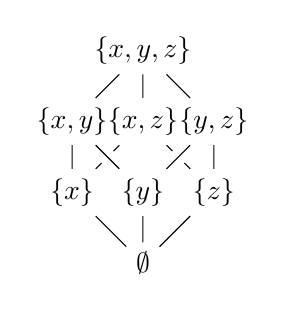
\begin{tikzpicture}[scale=0.45]
     
  \node (max) at (0,4) {$\{x,y,z\}$};
 \node (a) at (-2,2) {$\{x,y\}$};
 \node (b) at (0,2) {$\{x,z\}$};
 \node (c) at (2,2) {$\{y,z\}$};
 \node (d) at (-2,0) {$\{x\}$};
 \node (e) at (0,0) {$\{y\}$};
 \node (f) at (2,0) {$\{z\}$};
 \node (min) at (0,-2) {$\emptyset$};
 \draw (min) -- (d) -- (a) -- (max) -- (b) -- (f)
 (e) -- (min) -- (f) -- (c) -- (max)
 (d) -- (b);
 \draw[preaction={draw=white, -,line width=6pt}] (a) -- (e) -- (c);
          
  \end{tikzpicture}
	\caption{Hasse diagram}
	\end{figure}
\end{exampleblock}
\end{frame}
\begin{frame}{Lattice Theory}
\begin{definition}[least upper bound or join]
	A subset $S \subseteq P$ has a least upper bound (denoted $\sqcup S$ ) for     $(P,\preceq)$ if and only if:
	\begin{itemize} 
	\item  $\sqcup S \in P$ (the lub is an element of P)
	\item $ \forall x \in S~.~ x \preceq \sqcup S$ (the lub is an upper bound)
	\item $ \forall x \in S ~.~x \preceq u \Rightarrow \sqcup S \preceq u$ (\textbf{"minimum"} of the upper bounds)
\end{itemize}
\end{definition}
\begin{exampleblock}{Example:$(\mathcal{P}_S\{x,y,z\}, \subseteq)$}
	\begin{columns}
		\column{0.4\linewidth}
 	
   \tiny
  \usetikzlibrary{trees,shapes,decorations}
  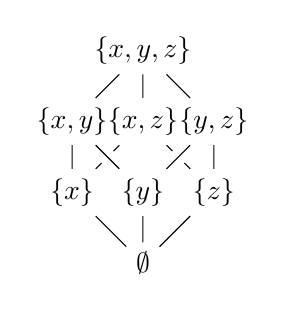
\begin{tikzpicture}[scale=0.45]
     
  \node (max) at (0,4) {$\{x,y,z\}$};
 \node (a) at (-2,2) {$\{x,y\}$};
 \node (b) at (0,2) {$\{x,z\}$};
 \node (c) at (2,2) {$\{y,z\}$};
 \node (d) at (-2,0) {$\{x\}$};
 \node (e) at (0,0) {$\{y\}$};
 \node (f) at (2,0) {$\{z\}$};
 \node (min) at (0,-2) {$\emptyset$};
 \draw (min) -- (d) -- (a) -- (max) -- (b) -- (f)
 (e) -- (min) -- (f) -- (c) -- (max)
 (d) -- (b);
 \draw[preaction={draw=white, -,line width=6pt}] (a) -- (e) -- (c);
          
  \end{tikzpicture}
 \column{0.6\linewidth}
 \footnotesize
 \begin{itemize}
 	\item  $\sqcup\{\{x\},\{z\}\}= \{y,z\}$
 	\item  $\sqcup\{\{x\},\{x,z\}\}=\{x,z\}$
 	\item  $\sqcup\{\emptyset,\{x,y,z\}\}=$??
 	\item  $\sqcup \{\{x\},\{y,z\}\}=$ ??
 \end{itemize}
	\end{columns}
\end{exampleblock}
\end{frame}


\begin{frame}{Lattice Theory}
\begin{definition}[greatest lower bound or meet]
	A subset $S \subseteq P$ has an greatest lower bound (denoted $\sqcap S$ ) for     $(P,\preceq)$ if and only if:
	\begin{itemize} 
		\item  $\sqcap S \in P$ (the glb is an element of P)
		\item $ \forall x \in S~.~   \sqcap S \preceq x$ (the lub is a lower bound)
		\item $ \forall x \in S ~.~l \preceq x \Rightarrow l \preceq \sqcap S  $ (\textbf{"maximum"} of the lower bounds)
	\end{itemize}
\end{definition}
\begin{exampleblock}{Example:$(\mathcal{P}_S\{x,y,z\}, \subseteq)$}
	\begin{columns}
		\column{0.4\linewidth}
		  \tiny
  \usetikzlibrary{trees,shapes,decorations}
  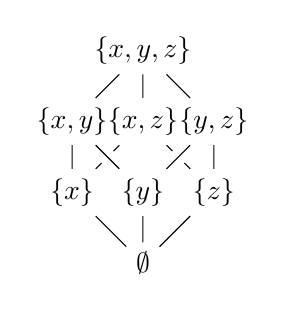
\begin{tikzpicture}[scale=0.45]
     
  \node (max) at (0,4) {$\{x,y,z\}$};
 \node (a) at (-2,2) {$\{x,y\}$};
 \node (b) at (0,2) {$\{x,z\}$};
 \node (c) at (2,2) {$\{y,z\}$};
 \node (d) at (-2,0) {$\{x\}$};
 \node (e) at (0,0) {$\{y\}$};
 \node (f) at (2,0) {$\{z\}$};
 \node (min) at (0,-2) {$\emptyset$};
 \draw (min) -- (d) -- (a) -- (max) -- (b) -- (f)
 (e) -- (min) -- (f) -- (c) -- (max)
 (d) -- (b);
 \draw[preaction={draw=white, -,line width=6pt}] (a) -- (e) -- (c);
          
  \end{tikzpicture}
		\column{0.6\linewidth}
		\footnotesize
		\begin{itemize}
			\item  $\sqcap\{\{x\},\{z\}\}= \emptyset$
			\item  $\sqcap\{\{x\},\{x,z\}\}=\{x\}$
			\item  $\sqcap\{\emptyset,\{x,y,z\}\}=$??
			\item  $\sqcap \{\{x\},\{y,z\}\}=$ ??
		\end{itemize}
	\end{columns}
\end{exampleblock}
\end{frame}

\begin{frame}{Lattice Theory}
\begin{definition}[Complete Lattice]
	A partial order $(P,\preceq)$ is a complete lattice if and only if for every  $S    \subseteq P$ the $\sqcup S$ and $\sqcap S$ are  defined.
\end{definition}

\begin{definition}[Least element and greatest element]
	A complete lattice  $(P,\preceq)$ has a maximal element $\top = \sqcup P$ and a minimal element  $\bot = \sqcap P$
\end{definition}

\begin{exampleblock}{Example:$(\mathcal{P}_S\{x,y,z\}, \subseteq)$ is a complete lattice}
	\begin{columns}
		\column{0.4\linewidth}
		  \tiny
  \usetikzlibrary{trees,shapes,decorations}
  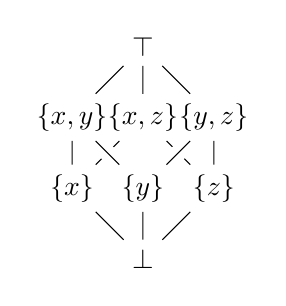
\begin{tikzpicture}[scale=0.45]
     
  \node (max) at (0,4) {$\top$};
 \node (a) at (-2,2) {$\{x,y\}$};
 \node (b) at (0,2) {$\{x,z\}$};
 \node (c) at (2,2) {$\{y,z\}$};
 \node (d) at (-2,0) {$\{x\}$};
 \node (e) at (0,0) {$\{y\}$};
 \node (f) at (2,0) {$\{z\}$};
 \node (min) at (0,-2) {$\bot$};
 \draw (min) -- (d) -- (a) -- (max) -- (b) -- (f)
 (e) -- (min) -- (f) -- (c) -- (max)
 (d) -- (b);
 \draw[preaction={draw=white, -,line width=6pt}] (a) -- (e) -- (c);
          
  \end{tikzpicture}
		\column{0.6\linewidth}
		\footnotesize
		\begin{itemize}
			\item  $\top = \sqcup \mathcal{P}_S\{x,y,z\}=\{x,y,z\}$
		     \item  $\bot = \sqcap \mathcal{P}_S\{x,y,z\}=\emptyset$
		\end{itemize}
	\end{columns}
\end{exampleblock}
\end{frame}

\begin{frame}{Lattice Theory}{Function monotonicity and fixed point}
\begin{definition}[Increasing function]
	A function $F: P \rightarrow P$ is said to be increasing over $(P,\preceq) $ (written  $F: P \xrightarrow{\scriptscriptstyle \nearrow} P$) if only if:
	\begin{itemize}
		\item $\forall x, y \in P.~x \preceq y \Rightarrow F(x) \preceq F(y)$
	\end{itemize}
\end{definition}

\begin{definition}[Function fixpoint]
	A function $F: P\rightarrow P$ has a fixpoint $\phi$ if and only if: 
	\begin{itemize}
		\item $\phi \in P$.
		\item $F(\phi)=\phi$
	\end{itemize}
\end{definition}



\begin{exampleblock}{Example: fixed point}
let 	$f :\mathbb{Z}  \rightarrow \mathbb{Z} , f(x)= x^2 - 3x +4 $\\
$f(2)=2$ and $f(f(f...(2)))=2$\\

$g :\mathbb{Z}  \rightarrow \mathbb{Z} , g(x)= x^2$ ??
\end{exampleblock}
\end{frame}

\begin{frame}{Lattice Theory}{Tarski theorem}
\begin{theorem}[Fixpoint theorem:Tarski Knaster]
For a complete lattice $(P,\preceq)$ and a function  $f: P  \xrightarrow{\scriptscriptstyle \nearrow} P$ we have:
\begin{enumerate}
\item f is guaranteed to have a fixpoint $\phi$.
\item f may have several fixpoints, from which a least fixpoint $lfp_f$ and a $gfp_f$.
\item  $lfp_f= \sqcup \{f^k (\bot). k \in \mathbb{N}\}$ \\( where $  \scriptstyle f^k(x)=f(f^{k-1}(x))$.)  
\end{enumerate}
\end{theorem}
\centering 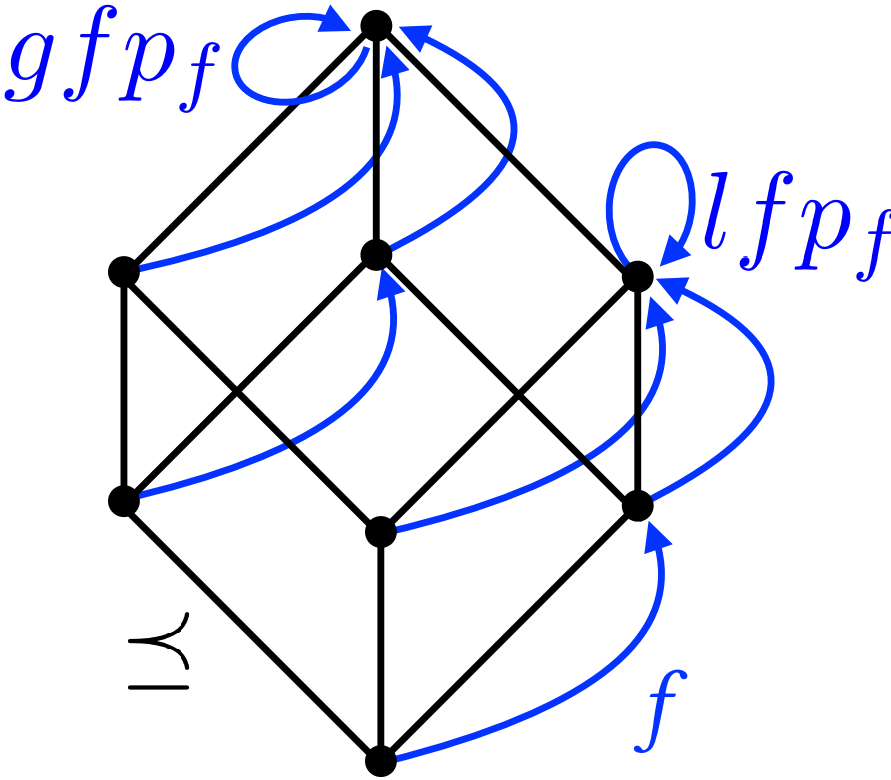
\includegraphics[scale=0.25]{content/images/static-analysis/lfp.png}
\end{frame}


\begin{frame}{Data Flow Analysis meets Tarski Theorem}
\begin{itemize}
	\item If the domain of values $\mathbb{V}$ can for a  lattice($\mathbb(V),\preceq $). 
	\item If  the transfer function $Tf: \mathbb{V}  \xrightarrow{\scriptscriptstyle \nearrow} \mathbb{V} $.
	\item Then we are guaranteed to reach a least fixpoint, which is the most precise solution in $\mathbb{V}$.
	\item Then ($ \mathbb{V}, Tf, \sqcup_ \preceq)$ a \textcolor{blue}{monotonic framework}.
	\item There is no generic monotonic framework for constant propagation.
	\item The difficulty is to design a suitable $\mathbb{V}, Tf$  program (represented by the set of program labels $\mathbb{L}$ ). 
	\item Precision vs. convergence.
\end{itemize}
\end{frame}


\begin{frame}{Monotonic Framework Example}

\begin{columns}
	\column{0.4\linewidth}
	\begin{figure}
		\centering  \tiny
  \usetikzlibrary{trees,shapes,decorations}
  \begin{tikzpicture}[%
    ->,
    >=stealth,
    node distance=0.3cm,
    noname/.style={%
      rectangle,
      minimum width=5em,
      minimum height=2em,
      draw
    }
  ]
    \node[noname] (1)                                             {[ x = 1; ] $l_1$};
    \node[noname] (2) [below=of 1]                                {[ while(??) ] $l_2$};
    \node[noname] (3) [below = 1cm of 2]                                {[ x = x+1; ] $l_3$};
    \node[noname] (4) [below right= 1cm of 2]                                {[ ;; ] $l_4$};
    
   
    

      \path 
   (1) edge                          node {} (2)
   (2) edge     [bend right=45pt]                     node  [yshift=5pt,right]{yes} (3)
   (2) edge                                         node  [yshift=5pt,right]{no} (4)
   (3) edge [bend right=45pt]                        node {} (2);
 
          
  \end{tikzpicture}\\
		\vspace{1cm}
		%\lstinputlisting[language=C, basicstyle =\scriptsize]{content/images/static-analysis/whileloop.c}
		\centering  \tiny
  \usetikzlibrary{trees,shapes,decorations}
  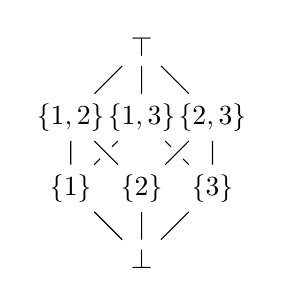
\begin{tikzpicture}[scale=0.45]
     
  \node (mam) at (0,4) {$\top$};
 \node (a) at (-2,2) {$\{1,2\}$};
 \node (b) at (0,2) {$\{1,3\}$};
 \node (c) at (2,2) {$\{2,3\}$};
 \node (d) at (-2,0) {$\{1\}$};
 \node (e) at (0,0) {$\{2\}$};
 \node (f) at (2,0) {$\{3\}$};
 \node (min) at (0,-2) {$\bot$};
 \draw (min) -- (d) -- (a) -- (mam) -- (b) -- (f)
 (e) -- (min) -- (f) -- (c) -- (mam)
 (d) -- (b);
 \draw[preaction={draw=white, -,line width=6pt}] (a) -- (e) -- (c);
          
  \end{tikzpicture}
	\end{figure}
	\column{0.6\linewidth}

	What is the result???
	
\end{columns}
\end{frame}

\begin{frame}{Monotonic Framework Example}

\begin{columns}
	\column{0.4\linewidth}
	\begin{figure}
	\centering  \tiny
  \usetikzlibrary{trees,shapes,decorations}
  \begin{tikzpicture}[%
    ->,
    >=stealth,
    node distance=0.3cm,
    noname/.style={%
      rectangle,
      minimum width=5em,
      minimum height=2em,
      draw
    }
  ]
    \node[noname] (1)                                             {[ x = 1; ] $l_1$};
    \node[noname] (2) [below=of 1]                                {[ while(??) ] $l_2$};
    \node[noname] (3) [below = 1cm of 2]                                {[ x = x+1; ] $l_3$};
    \node[noname] (4) [below right= 1cm of 2]                                {[ ;; ] $l_4$};
    
   
    

      \path 
   (1) edge                          node {} (2)
   (2) edge     [bend right=45pt]                     node  [yshift=5pt,right]{yes} (3)
   (2) edge                                         node  [yshift=5pt,right]{no} (4)
   (3) edge [bend right=45pt]                        node {} (2);
 
          
  \end{tikzpicture}\\
	\vspace{1cm}
	%\lstinputlisting[language=C, basicstyle =\scriptsize]{content/images/static-analysis/whileloop.c}
	\centering  \tiny
  \usetikzlibrary{trees,shapes,decorations}
  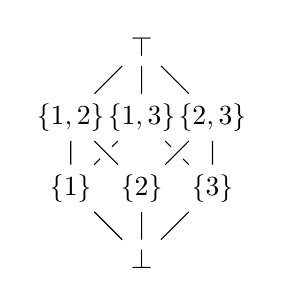
\begin{tikzpicture}[scale=0.45]
     
  \node (mam) at (0,4) {$\top$};
 \node (a) at (-2,2) {$\{1,2\}$};
 \node (b) at (0,2) {$\{1,3\}$};
 \node (c) at (2,2) {$\{2,3\}$};
 \node (d) at (-2,0) {$\{1\}$};
 \node (e) at (0,0) {$\{2\}$};
 \node (f) at (2,0) {$\{3\}$};
 \node (min) at (0,-2) {$\bot$};
 \draw (min) -- (d) -- (a) -- (mam) -- (b) -- (f)
 (e) -- (min) -- (f) -- (c) -- (mam)
 (d) -- (b);
 \draw[preaction={draw=white, -,line width=6pt}] (a) -- (e) -- (c);
          
  \end{tikzpicture}
    \end{figure}
	\column{0.6\linewidth}
	\begin{enumerate}\scriptsize
		\item $ \scriptstyle in_{l3}=in_{l2}=in_{l1}=\bot$ \scriptsize \textcolor{blue}{(initialization)}
		\item $ \scriptstyle  x_{l1}^1 =Tf_{l1}^1 (in_{l1})= \{1\}$
		\item $ \scriptstyle in_{l2}^1 = \sqcup(out_{l1},out_{l2})=\sqcup(\{1\}, \bot) =\{1\} $
		\item $ \scriptstyle x_{l3}^1= in_{l2}^1+ \{1\} = \{2\} $
		\item $ \scriptstyle in_{l2}^2 = \sqcup(1, 2) = \{1,2\}$
		\item $ \scriptstyle x_{l3}^2= in_{l2}^2+1 = \{1,2\} + \{1\} =\{2,3\}$
		\item $ \scriptstyle in_{l2}^2 = \sqcup(\{2,3\}, \{1\}) = \top \wedge x_{l2}^2=in_{l2}^2 $
		\item $\scriptstyle x_{l3}^3 =Tf_{l3}^3(\top)=\top $ \scriptsize \textcolor{blue}{(fixpoint reached) }
	\end{enumerate}
     \scriptsize
     $\top$ means the set of all possible values or the result is failing(all the possible values).\\
     the result will be the same of all the possible set lattices of $ ( S \subset \mathbb{Z}, \subseteq)$ if the iterations terminates. 
     
\end{columns}
\end{frame}

\begin{frame}{Data Flow: Wrap-Up}
\begin{itemize}
\item Monotonic frameworks ensures data flow analyses termination or \textcolor{blue}{Inductive program verification}.
\item The analysis is ensured by induction over the collecting semantics of the programming language.
\item The induction is defined because of the fixpoint theorem.
\item The results are not always precise and hard to tune.
\item Another way to analyse : approximating the programs properties.
\item \textcolor{blue}{Abstract program analysis}: analysis on Abstract domains to get meaningful approximations than the result concrete domains.
\end{itemize}
\end{frame}

\section{Analysis by Abstract Interpretation}
\begin{frame}{By Patrick and Radia Cousot}
\centering

\includegraphics[scale=0.60]{content/images/static-analysis/Abstractcousot.png}
\end{frame}


\begin{frame}{What is on the program}
\begin{itemize}
	\item Informal introduction.
	\item Galois connection for abstract interpretation.
	\item Interval abstract domain.
	\item widening, narrowing.
\end{itemize}
\end{frame}



\begin{frame}{Informal Introduction:}
\begin{itemize}
	\item Abstractions are an intuitive notion.
	\item Abstraction is on abstract domains.
	\item $[-\infty, +\infty] $ is an abstraction of $\mathbb{Z}$ in the interval domain. 
	\item Negative is an abstraction of $-2$ in the sign domain.
	\item Abstraction is an approximation.
\end{itemize}
\end{frame}



\begin{frame}{Undecidability}
\textit{"All interesting properties of the behavior of programs written in common programming languages are mathematically \textbf{undecidable}."} From Rice's Theorem [1953]

\textbf{Undecidable:}
\begin{itemize}
	\item \textbf{Among the solutions}: 
	\begin{enumerate}
		\item Identify a subclass of programs for which the verification problem is decidable.
		\item \textcolor{blue}{Approximate (Partial correctness, sound approximation)}. 
		\item Use dynamic methods to complement.		
	\end{enumerate}
\item \textcolor{blue}{Soundness}:The software contains a bug $\Rightarrow$  Run of the algorithm will detect it. \textbf{(No False negative)}.
\item What is a sound approximation?
\end{itemize} 
\end{frame}


\begin{frame}{Informal Introduction: Over/under Approximations}
\centering\documentclass[tikz,border=2mm]{standalone}
\begin{document}
\begin{tikzpicture}
\draw[help lines, color=gray!30, dashed] (-4.9,-4.9) grid (4.9,4.9);
\draw[->,ultra thick] (-5,0)--(5,0) node[right]{$x$};
\draw[->,ultra thick] (0,-5)--(0,5) node[above]{$y$};

\end{tikzpicture}
\end{document}
\begin{itemize}
	\item \textcolor{blue}{Values computed by the program}
	\item \textbf{Not always analysable: $\top$} is the result of the data flow analysis.
	\item We need to approximate, but why?

\end{itemize}
\end{frame}

\begin{frame}{Informal Introduction: Approximations}
\centering
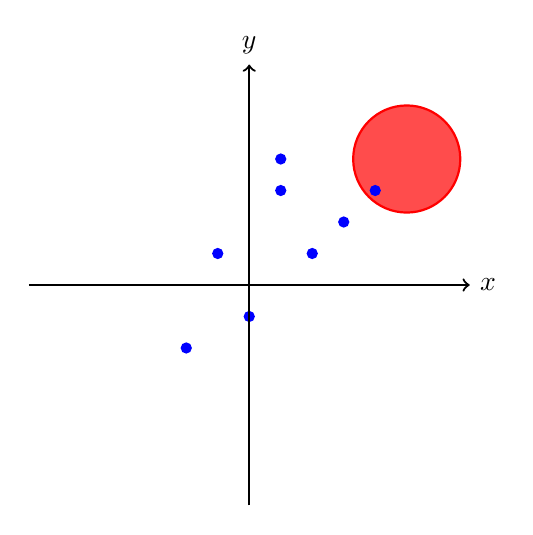
\begin{tikzpicture}[thick, scale=0.4,dot/.style={fill=blue,circle,minimum size=1pt}]




%\filldraw [fill=orange!10,draw=orange,thick] (0,1) circle (5.4);

%\filldraw [fill=yellow!70,draw=yellow,thick] (0,1) circle (3);
%\filldraw [fill=green!10,draw=green,thick]
%(-2.3, -3.3) rectangle (4.5, 4.5);
\filldraw [fill=red!70,draw=red,thick] (5,4) circle (1.70);



\filldraw [blue] (-1,1) circle (4pt)
(1,3) circle  (4pt)
(3,2) circle (4pt)
(4,3) circle (4pt)
(1,3) circle (4pt)
(1,4) circle (4pt)
(0,-1) circle (4pt)
%(2,-3) circle (4pt)
(2,1) circle (4pt)
(-2,-2) circle (4pt);
\draw[->, thick] (-7,0)--(7,0) node[right]{$x$};
\draw[->, thick] (0,-7)--(0,7) node[above]{$y$};


\end{tikzpicture}

\begin{itemize}
	\item \textcolor{blue}{Values computed by the program}
	\item \textbf{Not always analysable: when $\top$} is the analysis result.
	\item \textcolor{red}{ Bad states: causing bugs or violating a property.}
	\item We need to approximate.
\end{itemize}
\end{frame}

\begin{frame}{Informal Introduction: Over-/under-approximations}
\centering
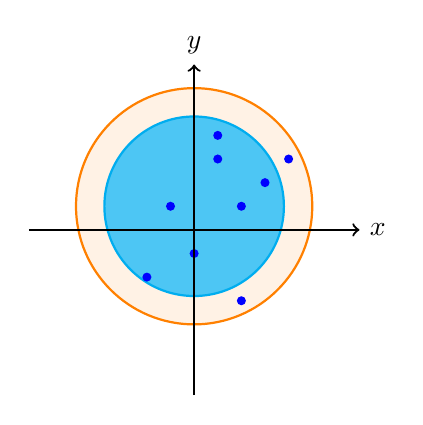
\begin{tikzpicture}[thick, scale=0.3,dot/.style={fill=blue,circle,minimum size=1pt}]




\filldraw [fill=orange!10,draw=orange,thick] (0,1) circle (5);

\filldraw [fill=cyan!70,draw=cyan,thick] (0,1) circle (3.8);
%\filldraw [fill=green!10,draw=green,thick]
%(-2.3, -3.3) rectangle (4.5, 4.5);
%\filldraw [fill=red!70,draw=red,thick] (5,4) circle (1.70);



\filldraw [blue] (-1,1) circle (4pt)
(1,3) circle  (4pt)
(3,2) circle (4pt)
(4,3) circle (4pt)
(1,3) circle (4pt)
(1,4) circle (4pt)
(0,-1) circle (4pt)
(2,-3) circle (4pt)
(2,1) circle (4pt)
(-2,-2) circle (4pt);

\draw[->, thick] (-7,0)--(7,0) node[right]{$x$};
\draw[->, thick] (0,-7)--(0,7) node[above]{$y$};

\end{tikzpicture}

\begin{itemize}
	\item \textcolor{blue}{Values computed by the program}.
	\item  \textcolor{orange}{Over-approximation}.
	\item  \textcolor{cyan}{Under-approximation}.
	\item \textbf{\textcolor{black}{ Which approximation is more suited for detecting "bad states"?}}
	
\end{itemize}
\end{frame}

\begin{frame}{Informal Introduction: Over/under-approximations}
\centering
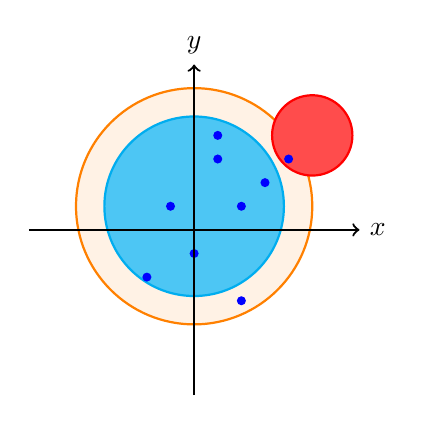
\begin{tikzpicture}[thick, scale=0.3,dot/.style={fill=blue,circle,minimum size=1pt}]




\filldraw [fill=orange!10,draw=orange,thick] (0,1) circle (5);

\filldraw [fill=cyan!70,draw=cyan,thick] (0,1) circle (3.8);
%\filldraw [fill=green!10,draw=green,thick]
%(-2.3, -3.3) rectangle (4.5, 4.5);
\filldraw [fill=red!70,draw=red,thick] (5,4) circle (1.70);



\filldraw [blue] (-1,1) circle (4pt)
(1,3) circle  (4pt)
(3,2) circle (4pt)
(4,3) circle (4pt)
(1,3) circle (4pt)
(1,4) circle (4pt)
(0,-1) circle (4pt)
(2,-3) circle (4pt)
(2,1) circle (4pt)
(-2,-2) circle (4pt);

\draw[->, thick] (-7,0)--(7,0) node[right]{$x$};
\draw[->, thick] (0,-7)--(0,7) node[above]{$y$};

\end{tikzpicture}

\begin{itemize}
	\item \textcolor{blue}{Values computed by the program}.
		\item \textcolor{red}{ Bad states: causing bugs or violating a property.}
	\item \textcolor{orange}{Over-approximation}, result is  \textbf{Yes}: $\surd$
	\item \textcolor{cyan}{Under-approximation},  result is  \textbf{No}:\textbf{ False negative}.   
	\item Over-approximation is sound.
\end{itemize}
\end{frame}
\begin{frame}{Informal Introduction: Over/under Approximations}
\centering
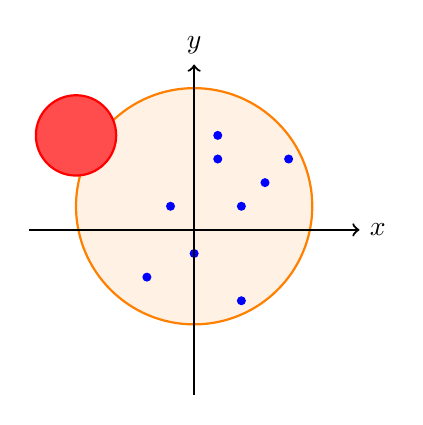
\begin{tikzpicture}[thick, scale=0.3,dot/.style={fill=blue,circle,minimum size=1pt}]




\filldraw [fill=orange!10,draw=orange,thick] (0,1) circle (5);
\filldraw [fill=red!70,draw=red,thick] (-5,4) circle (1.70);
%\filldraw [fill=cyan!70,draw=cyan,thick] (0,1) circle (3.8);
%\filldraw [fill=green!10,draw=green,thick]
%(-2.3, -3.3) rectangle (4.5, 4.5);




\filldraw [blue] (-1,1) circle (4pt)
(1,3) circle  (4pt)
(3,2) circle (4pt)
(4,3) circle (4pt)
(1,3) circle (4pt)
(1,4) circle (4pt)
(0,-1) circle (4pt)
(2,-3) circle (4pt)
(2,1) circle (4pt)
(-2,-2) circle (4pt);

\draw[->, thick] (-7,0)--(7,0) node[right]{$x$};
\draw[->, thick] (0,-7)--(0,7) node[above]{$y$};

\end{tikzpicture}

\begin{itemize}
	\item \textcolor{blue}{Values computed by the program}.
	\item \textcolor{red}{ Bad states: causing bugs or violating a property.}
	\item \textcolor{orange}{Over-approximation}, result is  \textbf{Yes}: False positive.  
	\item Over-approximation is not complete.
\end{itemize}
\end{frame}


\begin{frame}{What is Abstract interpretation?}
\begin{itemize}
	\item A \textcolor{blue}{mathematical theory} formalizing the abstraction of program semantic properties.
	\item Used to reason on and to calculate \textcolor{blue}{abstract program properties}.
	\item Applications: program semantics, verification, dynamic and \textcolor{blue}{static analysis of software}.
	\end{itemize}
\end{frame}

\begin{frame}{Informal Introduction:}
\begin{itemize}
	\item let \textcolor{blue}{$(\mathcal{C}, \preceq_c)$} a domain  of concrete values.
	\item let \textcolor{blue}{$(\mathcal{A}, \preceq_a)$} a domain of abstract values.
	\item Abstraction function \textcolor{blue}{$\alpha: \mathcal{C} \rightarrow \mathcal{A}$}.
	\item Concretization function \textcolor{blue}{$\gamma : \mathcal{A} \rightarrow \mathcal{B}$}.
	\item Suppose we want to verify a property \textcolor{blue}{$Prop \subset \mathcal{C}$}.
	\item Analyse the Program in the abstract domain \textcolor{blue}{$(\mathcal{A}, \preceq_a)$}, we need an abstract functions to obtain $Result^\sharp$.
	 \begin{enumerate}
	\item Concretize  \textcolor{blue}{$Result= \gamma(Result^\sharp)$} and check for \textcolor{blue}{$Prop$}.
	\item Abstract the property \textcolor{blue}{$Prop^\sharp = \alpha(Prop)$} and check with \textcolor{blue}{$Result^\sharp$}.
	\end{enumerate}
\end{itemize}
\end{frame}

\begin{frame}{First abstract domain: Sign abstract domain}
\begin{itemize}
	\item By Brahmagupta (born c.  598-670)) was an Indian mathematician and
	astronomer.
	\item Invented the rule of signs (including to compute with zero).
	\item Let's understand this reasoning in term of Abstract interpretation.
\end{itemize}
\end{frame}


\begin{frame}{First abstract domain: Sign abstract domain}
\centering 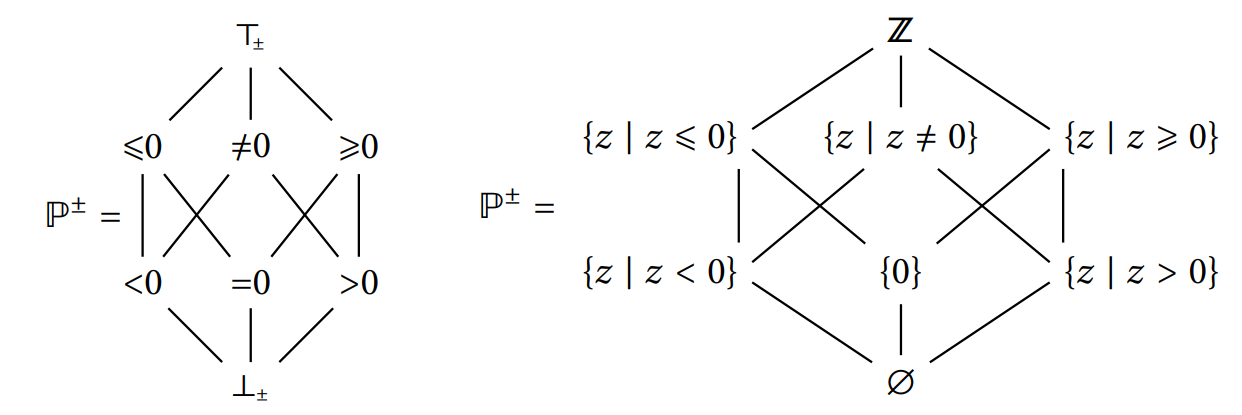
\includegraphics[scale=0.50]{content/images/static-analysis/sign.png}
\begin{itemize}
	\item $(\mathbb{P}^\pm, \subseteq_\pm)$ is the sign abstract domain.
	\item $(\mathcal{P_S}(\mathbb{Z}),\subseteq)$ be the concrete domain.
	\item The sign abstract domain is a complete lattice.
\end{itemize}
\end{frame}

\begin{frame}{First abstract domain: Sign abstract domain}
\begin{itemize}
	\item $(\mathbb{P}^\pm, \subseteq_\pm)$ is the sign abstract domain.
	\item $(\mathcal{P_S}(\mathbb{Z}),\subseteq)$ be the concrete domain.
	\item The abstraction function is defined as $\alpha^{\pm}: \mathbb{Z} \rightarrow \mathbb{P}^{\pm}+$:\newline
$\forall e \subseteq \mathbb{Z}: \alpha_\pm(e)     \left\{ \begin{array}{rcl}
\bot_{\pm} & \mbox{if}& e= \emptyset \\
=0  & \mbox{else if} & e \subseteq \{0\} \\
>0 & \mbox{else if} & e \subseteq \{x \in \mathbb{Z} |~ x >0\}\\
<0 & \mbox{else if} & e\subseteq \{x \in \mathbb{Z} |~ x <0\}\\
\leq 0 & \mbox{else if} & e\subseteq \{x \in \mathbb{Z} | ~x  \leq 0\}\\
\geq 0 & \mbox{else if} & e\subseteq \{x \in \mathbb{Z} |~ x  \geq 0\}\\
\neq 0 & \mbox{else if} & e\subseteq \{x \in \mathbb{Z} |~ x  \neq 0\}\\
\top_\pm & \mbox{else} & 
\end{array}\right.$
\end{itemize}
\begin{exampleblock}{Examples:}
	$    \begin{array}{l l}
\alpha^{\pm}(\{1,3,7\})=~>0 & \alpha^{\pm}(\{0,1,3,7\})=~\geq 0 \\
\alpha^{\pm}(\{-1,7\})=~ ?? & \alpha^{\pm}(\{-16,0,1,7\})=~ ?? \\
\end{array}$
\end{exampleblock}
\end{frame}

\begin{frame}{First abstract domain: Sign abstract domain}
\begin{itemize}
	\item $(\mathbb{P}^\pm, \subseteq_\pm)$ is the sign abstract domain.
	\item $(\mathcal{P_S}(\mathbb{Z}),\subseteq)$ be the concrete domain.
	\item The sign concretization function is defined as $\gamma_\pm:  \mathbb{P}^{\pm} \rightarrow \mathbb{Z}$:
	
	$    \begin{array}{l l}
\gamma^{\pm}(\bot^{\pm}) = \emptyset &  \gamma^{\pm}(=0)=\{0\} \\ 
\gamma_\pm(>0)=\{x \in \mathbb{Z} |~ x >0\}	 & \gamma_\pm(<0)=\{x \in \mathbb{Z} |~ x <0\} \\
\gamma_\pm(\leq0)=\{x \in \mathbb{Z} |~ x \leq 0\}	 & \gamma_\pm(\geq 0)=\{x \in \mathbb{Z} |~ x \geq 0\} \\
\gamma_\pm(\neq 0)=\{x \in \mathbb{Z} |~ x \neq 0\}	 & \gamma_\pm(\top^{\pm})=\mathbb{Z} \\
\end{array}.$
\end{itemize}
\end{frame}

\begin{frame}{Abstract interpretation: Galois connections}
\begin{definition}[Galois connection]
 $(\mathcal{C}, \preceq_c) \galois{\alpha}{\gamma} (\mathcal{A}, \preceq_a)$ is a Galois connection iff:
 \begin{enumerate}
 \item $\gamma$ is increasing;
 \item $\alpha$ is increasing;
 \item $\forall x \in \mathcal{C}~. ~x \preceq_c \gamma \comp \alpha(x)$ ($\gamma \comp \alpha$ is extensive)
 \item $\forall y \in \mathcal{A}~.~ \alpha \comp \gamma(y) \preceq_a y$ ($\alpha \comp \gamma$ is reductive)
 \end{enumerate}
\end{definition}

\begin{exampleblock}{Examples:$(\mathbb{Z}, \subseteq) \galois{\alpha_\pm}{\gamma_\pm} (\mathbb{P}_{\pm}, \subseteq_{\pm})$}
	
	$\begin{array}{l l l}
	\scriptstyle \gamma_\pm\comp \alpha_\pm (\{1,2,3\})= \{x \in \mathbb{Z} |~ x >0\} & \text{and} &\scriptstyle\alpha_\pm\comp \gamma_\pm(>0) =~>0  \\
	\scriptstyle \{1,2,3\} \subseteq  \{x \in \mathbb{Z} |~ x >0\} & \text{and}  & \scriptstyle>0 ~\subseteq_\pm~ >0
	\end{array}$
\end{exampleblock}
\end{frame}
	
\begin{frame}{Best abstract transfer function}
\begin{definition}[Best abstract transformer]
$(\mathcal{C}, \preceq_c) \galois{\alpha}{\gamma} (\mathcal{A}, \preceq_a)$ and $F:\mathcal{C} \rightarrow \mathcal{C}$, the best abstract function $F^{\scriptsize \sharp}_b: \mathcal{A}\rightarrow\mathcal{A}$ is defined as:
\begin{itemize}
	\item $F^{\scriptsize \sharp}_b(y) \triangleq \alpha \comp F \comp \gamma (y)$
\end{itemize}
\end{definition}

 \begin{alertblock}{The best abstract transfer function does not always exist:}
 	\begin{itemize}
	\item In practice, $\alpha \comp TF \comp \gamma$ is not computable or too complex.
	\item Also, sometimes either  $\alpha$/$\gamma$ is not defined.	
	\item The solution is to define  $ TF^{\scriptsize \sharp}_b\preceq_\sharp TF^{\scriptsize \sharp} $
    \end{itemize}
\end{alertblock}
\end{frame}


\begin{frame}{Collecting semantics for the sign abstract domain with 1 variable x}
\begin{itemize}
	\item \scriptsize The set of sign transfer functions is defined as: \\$in_{li}=\sqcup(x_{pre_{li}})$ and $ x_{l_i}= TF^{\scriptscriptstyle \pm}_{l_i}(in_{l_i})$\\
	$  TF^{\scriptscriptstyle \pm}_{l_i}(in_{l_i}) =     \left\{ \begin{array}{rcl}
\textstyle	in_{l_i} &  \mbox{\scriptsize if}& \textstyle l_i~\text{\scriptsize is}~while(B)~\mid~ if(B) ~\mid~;;   \\
\textstyle	\|a\|_{li}^{\scriptscriptstyle \pm}  & \mbox{\scriptsize if} & \textstyle l_i~\mbox{\scriptsize is}~x~=~a; \\
\scriptstyle	\|a\|_{li}^{\scriptscriptstyle \pm}~op_\pm~ \|b\|_{li}^{\scriptscriptstyle \pm}  & \mbox{\scriptsize if} &  \textstyle l_i~\mbox{\scriptsize is}~x~=~a~op_a~b; \\
	\dots & \mbox{if} & \dots
	\end{array}\right.$
	
	\item \scriptsize The abstract evaluation function:\\  $ \|a\|_{li}^{\scriptscriptstyle \pm} =     \left\{ \begin{array}{rcl}
	in_{l_i} & \mbox{ if}&  \text{x is a variable}   \\
	\gamma_{\pm}(a)  & \mbox{ if} &  \text{x is a a constant value} 
\end{array}\right.$
\item The set of abstract arithmetic operator: $op_\pm=\{+_{\scriptscriptstyle \pm}, -_{\scriptscriptstyle \pm}, \times_{\scriptscriptstyle \pm}\}$
\end{itemize}
\centering 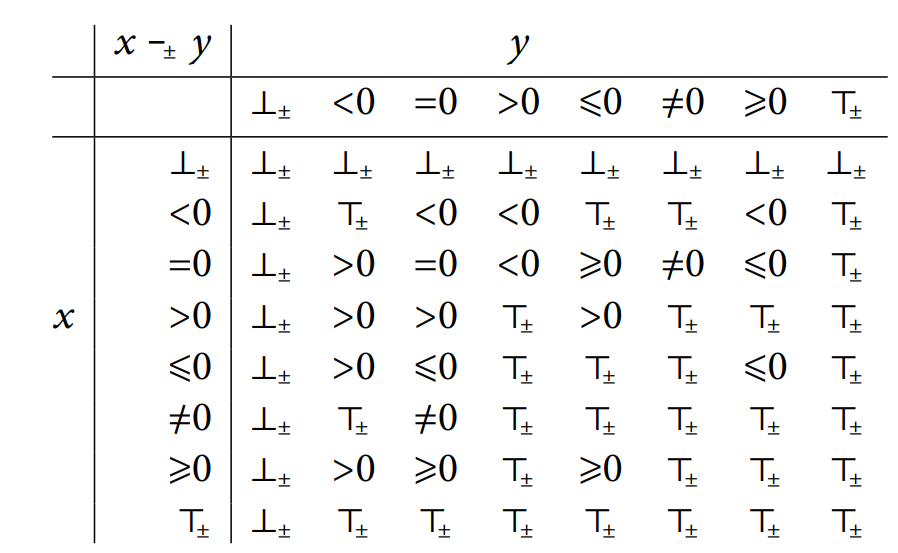
\includegraphics[scale=0.40]{content/images/static-analysis/minus-sign.png}
\end{frame}

\begin{frame}{While example in the sign domain:}
\begin{exampleblock}{while loop:1}
	\centering   \tiny
  \usetikzlibrary{trees,shapes,decorations}
  \begin{tikzpicture}[%
    ->,
    >=stealth,
    node distance=0.3cm,
    noname/.style={%
      rectangle,
      minimum width=5em,
      minimum height=2em,
      draw
    }
  ]
    \node[noname] (1)                                             {[ x = 1; ] $l_1$};
    \node[noname] (2) [below=of 1]                                {[ while(??) ] $l_2$};
    \node[noname] (3) [below = 1cm of 2]                                {[ x = x+1; ] $l_3$};
    \node[noname] (4) [below right= 1cm of 2]                                {[ ;; ] $l_4$};
    
   
    

      \path 
   (1) edge                          node {} (2)
   (2) edge     [bend right=45pt]                     node  [yshift=5pt,right]{yes} (3)
   (2) edge                                         node  [yshift=5pt,right]{no} (4)
   (3) edge [bend right=45pt]                        node {} (2);
 
          
  \end{tikzpicture}
	\centering 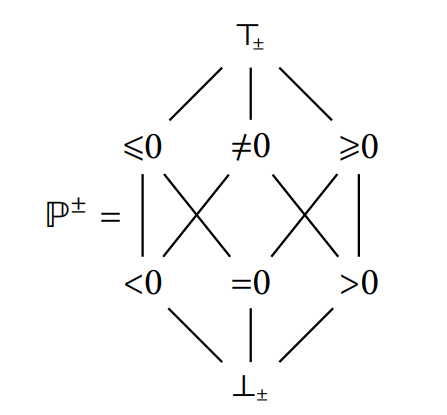
\includegraphics[scale=0.60]{content/images/static-analysis/sign1.png}
	
	\begin{itemize}
		\item Initialization: 
			\\ $\scriptsize in_{l_1}=in_{l_2}=in_{l_3}=in_{l_4}=~\bot^{\pm}$
			\\ $\scriptsize x_{l_1}^0 =~>0~;~~x_{l_2}^0 =~~>0~;~~x_{l_3}^0 =~~>0~;~~x_{l_4}^0 =~>0~~$
			
		\end{itemize}
\end{exampleblock}
\end{frame}

\begin{frame}{While example in the sign domain:}
\begin{exampleblock}{while loop:2}
	\centering   \tiny
  \usetikzlibrary{trees,shapes,decorations}
  \begin{tikzpicture}[%
    ->,
    >=stealth,
    node distance=0.3cm,
    noname/.style={%
      rectangle,
      minimum width=5em,
      minimum height=2em,
      draw
    }
  ]
    \node[noname] (1)                                             {[ x = 1; ] $l_1$};
    \node[noname] (2) [below=of 1]                                {[ while(??) ] $l_2$};
    \node[noname] (3) [below = 1cm of 2]                                {[ x = x+1; ] $l_3$};
    \node[noname] (4) [below right= 1cm of 2]                                {[ ;; ] $l_4$};
    
   
    

      \path 
   (1) edge                          node {} (2)
   (2) edge     [bend right=45pt]                     node  [yshift=5pt,right]{yes} (3)
   (2) edge                                         node  [yshift=5pt,right]{no} (4)
   (3) edge [bend right=45pt]                        node {} (2);
 
          
  \end{tikzpicture}
	\centering 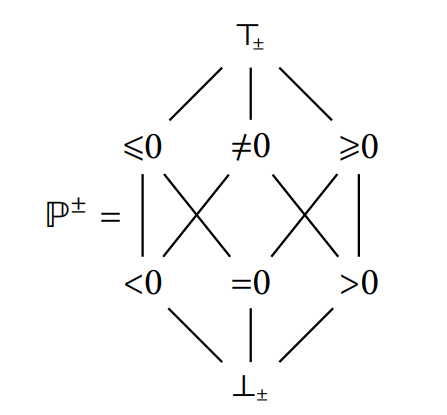
\includegraphics[scale=0.60]{content/images/static-analysis/sign1.png}
	
	\begin{itemize}
		\item Initialization: 
		\\ $\scriptsize in_{l_1}=in_{l_2}=in_{l_3}=in_{l_4}=\bot^{\pm}$
		\\ $\scriptsize x_{l_1}^0 =~>0~;~~x_{l_2}^0 =~>0~;~~x_{l_3}^0 =~>0~;~~x_{l_4}^0 =~>0~~~$
		
		\item First iteration: $x_{l_1}^1 = ~>0 = x_{l_1}^0 $ fixpoint for $l_1$ 
		\item Second iteration: $x_{l_2}^2 = ~>0  =  x_{l_2}^0 $ fixpoint for $l_2$ 
		\item Third iteration: $x_{l_3}^4 = ~>0 = x_{l_4}^0 $ fixpoint for $l_3$ 
		\item Fourth iteration $x_{l_4}^5 =~ >0 = x_{l_4}^0 $ fixpoint for $l_4$ and $worklist=\emptyset$
		\item The result of the analysis is: $>0$
	\end{itemize}
\end{exampleblock}
\end{frame}

\begin{frame}{While example1:}
\begin{exampleblock}{while loop:1}
	\centering   \tiny
  \usetikzlibrary{trees,shapes,decorations}
  \begin{tikzpicture}[%
    ->,
    >=stealth,
    node distance=0.3cm,
    noname/.style={%
      rectangle,
      minimum width=5em,
      minimum height=2em,
      draw
    }
  ]
    \node[noname] (1)                                             {[ x = 1; ] $l_1$};
    \node[noname] (2) [below=of 1]                                {[ while(??) ] $l_2$};
    \node[noname] (3) [below = 1cm of 2]                                {[ x = x+1; ] $l_3$};
    \node[noname] (4) [below right= 1cm of 2]                                {[ ;; ] $l_4$};
    
   
    

      \path 
   (1) edge                          node {} (2)
   (2) edge     [bend right=45pt]                     node  [yshift=5pt,right]{yes} (3)
   (2) edge                                         node  [yshift=5pt,right]{no} (4)
   (3) edge [bend right=45pt]                        node {} (2);
 
          
  \end{tikzpicture}
	\centering 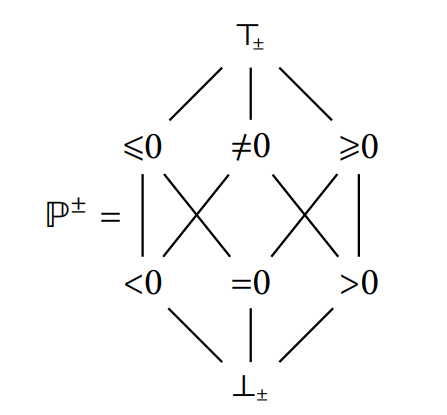
\includegraphics[scale=0.60]{content/images/static-analysis/sign1.png}
			\begin{enumerate}
				\item The abstract solution is: $Result^{\pm}~=~>0$ for  $(\mathbb{P}^\pm, \subseteq_\pm)$ with $TF^{\scriptscriptstyle \pm}$
				\item The concretization is : $\gamma_{\pm}(>0)= \{z \in \mathbb{Z} ~|~ z>0 \}$
				\item The result was $\top$ for $(\mathbb{Z}, \subseteq)$ with $TF$
			    \item $\gamma_{\pm}(Result^{\pm})=\{z \in \mathbb{Z} ~|~ z>0 \} \subseteq \top$  in the concrete domain.
			    \item The real values of the program are: $\{z \in \mathbb{Z} ~|~ z \geq 1 \} \equiv_{\mathbb{Z}} {\displaystyle \gamma}_{\pm}(Result^{\pm})$
			    \item Can we do better with another abstract domain for this program?
			    \item Are the results of $TF^\pm$ always more precise than $TF$??
				\end{enumerate}
	
\end{exampleblock}
\end{frame}

\begin{frame}{Precision ???}
\begin{exampleblock}{if example in the sign framework }
	Analyse the following program using $TF$ and $TF^{\pm}$, and compare their results.
\lstinputlisting[language=C, basicstyle =\tiny]{content/images/static-analysis/precision.c}
	\end{exampleblock}
\end{frame}


\begin{frame}{Interval domain:$(\mathcal{I}, \sqsubseteq )$}\
\centering 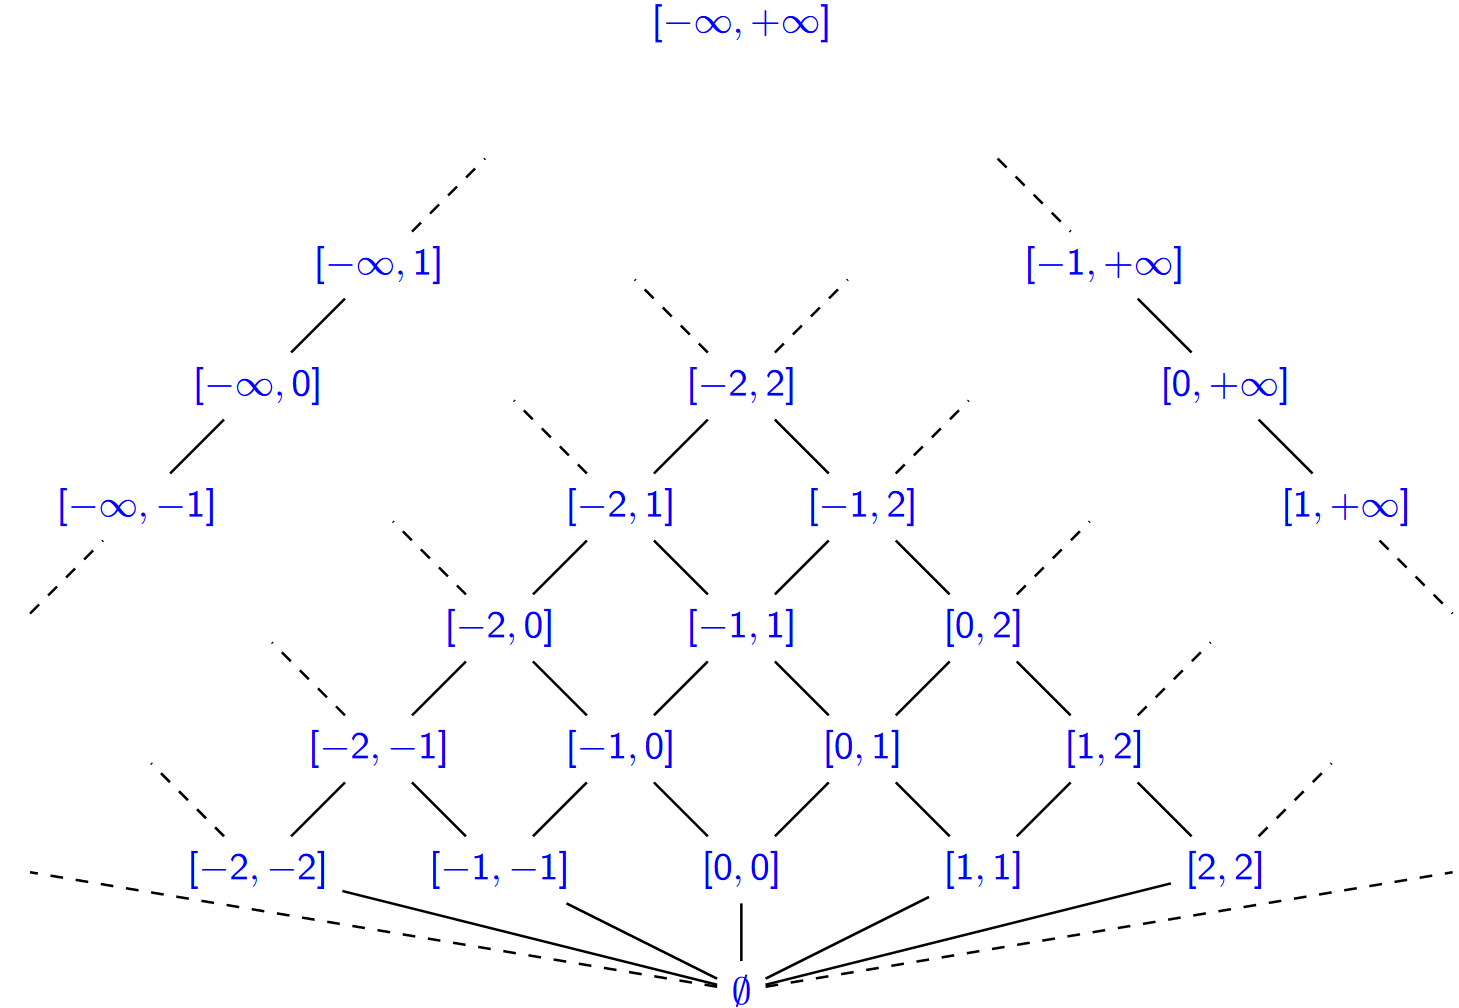
\includegraphics[scale=0.45]{content/images/static-analysis/interval.png}
\end{frame}

\begin{frame}{Interval domain:$(\mathcal{I}, \sqsubseteq )$}
\begin{itemize}
\item $(\mathcal{I}, \sqsubseteq )$ is a complete lattice.
\item $(\mathcal{I}, \sqsubseteq )$ with enumerable element but is countably infinite.
\item \textcolor{orange}{Problem 1}: can't infer the $\sqcup_{\scriptscriptstyle \sqsubseteq}$ from the Hasse diagram.
\item \textcolor{orange}{Problem 2}: ??
\end{itemize}
\end{frame}


\begin{frame}{Interval domain:$(\mathcal{I}, \sqsubseteq )$}
\begin{itemize}
	\item $(\mathcal{I}, \sqsubseteq )$ is a complete lattice.
	\item $(\mathcal{I}, \sqsubseteq )$ with enumerable elements but is \textcolor{orange}{countably infinite}.
	\item \textcolor{orange}{Problem 1}: can't infer the $\sqcup_{\scriptscriptstyle \sqsubseteq}$ from the Hasse diagram.
	\begin{itemize}
		\item Define $\sqcup_{\scriptscriptstyle \sqsubseteq}$
   \end{itemize}
	\item \textcolor{orange}{Problem 2}: ??
\end{itemize}
\end{frame}

\begin{frame}{Interval domain: join operator  $\sqcup_{\scriptscriptstyle \sqsubseteq}$}
\begin{itemize}
	\item Can be defined using  $\sqcup_\subseteq$ from $(\mathcal{P}_S(\mathbb{Z}), \subseteq)$.
	\item Can also be defined using $min$ and $max$ functions.
	\item $\sqcup_{\scriptscriptstyle \sqsubseteq}([a,b],[c,d])=[min(a,c),max(c,d)]$
	\item Set of axioms for $-\infty, \infty$:\\
	
	$  \forall x \in \mathbb{Z}     \left\{ \begin{array}{lcc}
	x  &  < & \infty  \\
	x  &  > & -\infty   \\
	-\infty &  < & \infty \\
\end{array}\right.$
\end{itemize}
\end{frame}

\begin{frame}{Interval domain: $\gamma_{\scriptscriptstyle\mathcal{I}}: \mathcal{I} \rightarrow \mathcal{P}_S(\mathbb{Z})$}
\begin{itemize}
	\item $\alpha_{\scriptscriptstyle\mathcal{I}}(x)=
	 \left\{ \begin{array}{lcc}
	\top^I~=~[-\infty,\infty]  &  \text{if} & x=\top  \\
	\bot^I~=~\emptyset  &  \text{if} & x=\bot \\
     I_x~=~[inf(x), sup(x)]   &  else &   \\
	\end{array}\right.$  
		\item $\gamma_{\scriptscriptstyle\mathcal{I}}(y)=
	\left\{ \begin{array}{lcl}
	\top &  \text{if} & y=\top^I  \\
	\bot~=~\emptyset  &  \text{if} & y=\bot^I \\
	\{x \in \mathbb{Z} ~|~ x \leq b \}&  \text{if} & y = [-\infty,b]  \\
	\{x \in \mathbb{Z} ~|~ a \leq x  \}&  \text{if} & y = [a,\infty]  \\
	\{x \in \mathbb{Z} ~|~ a \leq x \leq b\} &  \text{if} & y = [a,b]  \\
	\end{array}\right.$
\end{itemize}
\begin{exampleblock}{Examples:}
	
	$\begin{array}{l}
	 \gamma_{\scriptscriptstyle\mathcal{I}} \comp \alpha_{\scriptscriptstyle\mathcal{I}} (\{1,2,3\})= \gamma_{\scriptscriptstyle\mathcal{I}}([1,3])= {\scriptstyle \{x \in \mathbb{Z}~|~ 1 \leq x \leq 3\}} =\{1,2,3\}  \\
	 \{1,2,3\} =  \gamma_{\scriptscriptstyle\mathcal{I}} \comp \alpha_{\scriptscriptstyle\mathcal{I}} (\{1,2,3\})\\
 \gamma_{\scriptscriptstyle\mathcal{I}} \comp \alpha_{\scriptscriptstyle\mathcal{I}} (\{1,3\})= ??\\
	 \gamma_{\scriptscriptstyle\mathcal{I}} \comp \alpha_{\scriptscriptstyle\mathcal{I}} (\{x \in \mathbb{Z}~.~x\leq 1\})= ??
	\end{array}$\\
	
\end{exampleblock}
\end{frame}

\begin{frame}{Collecting semantics for the $(\mathcal{I},\sqsubseteq)$  domain with 1 variable x}
\begin{itemize}
	\item \scriptsize The set of Interval transfer functions is defined as:\\$in_{li}=\sqcup(x_{pre_{li}})$ and $ x_{l_i}= TF^{\scriptscriptstyle \mathcal{I}}_{l_i}(in_{l_i}),$\\ 
	$  TF^{\scriptscriptstyle \mathcal{I}}_{l_i}(in_{l_i}) =     \left\{ \begin{array}{rcl}
	\textstyle	in_{l_i} &  \mbox{\scriptsize if}& \textstyle l_i~\text{\scriptsize is}~while(B)~\mid~ if(B) ~\mid~;;   \\
	\textstyle	\|a\|_{li}^{\scriptscriptstyle \mathcal{I}}  & \mbox{\scriptsize if} & \textstyle l_i~\mbox{\scriptsize is}~x~=~a; \\
	\scriptstyle	\|a\|_{li}^{\scriptscriptstyle \mathcal{I}}~op_\mathcal{I}~ \|b\|_{li}^{\scriptscriptstyle \mathcal{I}}  & \mbox{\scriptsize if} &  \textstyle l_i~\mbox{\scriptsize is}~x~=~a~op_a~b; \\
	\dots & \mbox{if} & \dots
	\end{array}\right.$
	
	\item \scriptsize The abstract evaluation function:\\  $ \|a\|_{li}^ {\scriptscriptstyle \mathcal{I}} =     \left\{ \begin{array}{rcl}
	in_{l_i} & \mbox{ if}&  \text{x is a variable}   \\
	\gamma^{\scriptscriptstyle \mathcal{I}}(a)  & \mbox{ if} &  \text{x is a a constant value} 
	\end{array}\right.$
%	\item The set of abstract arithmetic operator:
%	 $op_{\scriptscriptstyle \mathcal{I}}\in \{+_{\scriptscriptstyle \mathcal{I}}, -_{\scriptscriptstyle \mathcal{I}}, \times_{\scriptscriptstyle \mathcal{I}}\}$
\end{itemize}

\end{frame}

\begin{frame}{Collecting semantics for the $(\mathcal{I},\sqsubseteq)$  domain with 1 variable x}
\begin{itemize}
	\item \scriptsize The set of Interval transfer functions is defined as: \\$in_{li}=\sqcup(x_{pre_{li}})$ and $ x_{l_i}= TF^{\scriptscriptstyle \mathcal{I}}_{l_i}(in_{l_i})$\\
	$  TF^{\scriptscriptstyle \mathcal{I}}_{l_i}(in_{l_i}) =     \left\{ \begin{array}{rcl}
	\textstyle	in_{l_i} &  \mbox{\scriptsize if}& \textstyle l_i~\text{\scriptsize is}~while(B)~\mid~ if(B) ~\mid~;;   \\
	\textstyle	\|a\|_{li}^{\scriptscriptstyle \mathcal{I}}  & \mbox{\scriptsize if} & \textstyle l_i~\mbox{\scriptsize is}~x~=~a; \\
	\scriptstyle	\|a\|_{li}^{\scriptscriptstyle \mathcal{I}}~op_\mathcal{I}~ \|b\|_{li}^{\scriptscriptstyle \mathcal{I}}  & \mbox{\scriptsize if} &  \textstyle l_i~\mbox{\scriptsize is}~x~=~a~op_a~b; \\
	\dots & \mbox{if} & \dots
	\end{array}\right.$
	
	\item \scriptsize The abstract evaluation function:\\  $ \|a\|_{li}^ {\scriptscriptstyle \mathcal{I}} =     \left\{ \begin{array}{rcl}
	in_{l_i} & \mbox{ if}&  \text{x is a variable}   \\
	\gamma^{\scriptscriptstyle \mathcal{I}}(a)  & \mbox{ if} &  \text{x is a a constant value} 
	\end{array}\right.$
		\item The set of abstract arithmetic operator:
		 $op_{\scriptscriptstyle \mathcal{I}}\in \{+_{\scriptscriptstyle \mathcal{I}}, -_{\scriptscriptstyle \mathcal{I}}, \times_{\scriptscriptstyle \mathcal{I}}\}$.\\
		 $op_{\scriptscriptstyle \mathcal{I}}: \mathcal{I} \times \mathcal{I} \rightarrow \mathcal{I}:$
		 
		 
		\begin{itemize}
		 	\item $\bot{\scriptscriptstyle \mathcal{I}} ~~op_{\scriptscriptstyle \mathcal{I}}~~ [a,b] = [a,b]~ op_{\scriptscriptstyle \mathcal{I}} ~\bot{\scriptscriptstyle \mathcal{I}} = ~\bot{\scriptscriptstyle \mathcal{I}}  $
		 	\item $[a,b] +_{\scriptscriptstyle \mathcal{I}}[c,d] = [a+c,b+d]$
		 	\item $[a,b] -_{\scriptscriptstyle \mathcal{I}}[c,d] = [a-d,b-c]$
		 	\item $ [a,b] \times_{\scriptscriptstyle \mathcal{I}}[c,d]=[min(B), max(B)] $\\ with $ B = \{(a \times c), (a \times d), (b\times c), (b \times d)\}$
		 \end{itemize}
		 
\end{itemize}
\end{frame}

\begin{frame}{While Example in the Interval Domain:}
\begin{exampleblock}{while loop:1}
	\centering   \tiny
  \usetikzlibrary{trees,shapes,decorations}
  \begin{tikzpicture}[%
    ->,
    >=stealth,
    node distance=0.3cm,
    noname/.style={%
      rectangle,
      minimum width=5em,
      minimum height=2em,
      draw
    }
  ]
    \node[noname] (1)                                             {[ x = 1; ] $l_1$};
    \node[noname] (2) [below=of 1]                                {[ while(??) ] $l_2$};
    \node[noname] (3) [below = 1cm of 2]                                {[ x = x+1; ] $l_3$};
    \node[noname] (4) [below right= 1cm of 2]                                {[ ;; ] $l_4$};
    
   
    

      \path 
   (1) edge                          node {} (2)
   (2) edge     [bend right=45pt]                     node  [yshift=5pt,right]{yes} (3)
   (2) edge                                         node  [yshift=5pt,right]{no} (4)
   (3) edge [bend right=45pt]                        node {} (2);
 
          
  \end{tikzpicture}
	\centering 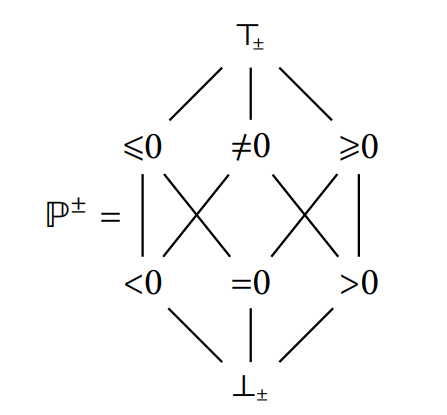
\includegraphics[scale=0.60]{content/images/static-analysis/sign1.png}
	
	\begin{itemize}
		\item Initialization: 
		\\ $\scriptsize in_{l_1}=in_{l_2}=in_{l_3}=in_{l_4}=\bot^{\mathcal{I}}$
		\\ $\scriptsize x_{l_1}^0 =?? ;~~x_{l_2}^0 =~??~;~~x_{l_3}^0 =~??~;~~x_{l_4}^0 =~??$
	\end{itemize}
\end{exampleblock}
\end{frame}

\begin{frame}{While Example in the Interval Domain:}
\begin{exampleblock}{while loop:2}
	\centering   \tiny
  \usetikzlibrary{trees,shapes,decorations}
  \begin{tikzpicture}[%
    ->,
    >=stealth,
    node distance=0.3cm,
    noname/.style={%
      rectangle,
      minimum width=5em,
      minimum height=2em,
      draw
    }
  ]
    \node[noname] (1)                                             {[ x = 1; ] $l_1$};
    \node[noname] (2) [below=of 1]                                {[ while(??) ] $l_2$};
    \node[noname] (3) [below = 1cm of 2]                                {[ x = x+1; ] $l_3$};
    \node[noname] (4) [below right= 1cm of 2]                                {[ ;; ] $l_4$};
    
   
    

      \path 
   (1) edge                          node {} (2)
   (2) edge     [bend right=45pt]                     node  [yshift=5pt,right]{yes} (3)
   (2) edge                                         node  [yshift=5pt,right]{no} (4)
   (3) edge [bend right=45pt]                        node {} (2);
 
          
  \end{tikzpicture}
	\centering 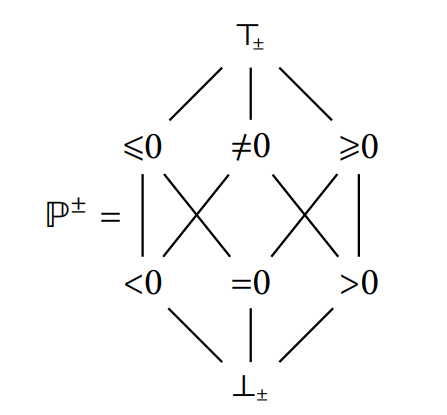
\includegraphics[scale=0.60]{content/images/static-analysis/sign1.png}
	
	\begin{itemize}
		\item result??: 
		\\ $\scriptsize in_{l_1}~=~in_{l_2}=in_{l_3}=in_{l_4}=\bot^{\mathcal{I}}$
		\\ $\scriptsize x_{l_1}^0 = [1,1] ;~~x_{l_2}^0 =~[1,1]~;~~x_{l_3}^0 =~[2,2]~;~~x_{l_4}^0 =~[1,1]$\\
		 $\scriptsize x_{l_4}^1 = [1,2] ;~~x_{l_4}^2 =~[1,3]~;~~x_{l_4}^3 =~[1,4]~;$
		\\ $\scriptsize x_{l_4}^4= [1,5] ;...;~~x_{l_4}^k =~[1,k+1]~;$
		\item Analysis does not terminate again;
		\item Intuition is that the result is $[1,\infty]$;
	\end{itemize}
\end{exampleblock}
\end{frame}


\begin{frame}{Widening $\nabla$: Fixpoint Accelerator}
\begin{itemize}
	\item $lim_{x\to +\infty} (x ~+~1) = +\infty$ because $x~+~1$ is $\nearrow$
	\item The $\nabla$  for intervals is defined as : $\nabla : \mathcal{I} \times \mathcal{I} \rightarrow \mathcal{I}$\\
	\begin{enumerate}
	\item $[a,b] ~\nabla ~\bot_\mathcal{I}= ~\bot_\mathcal{I} ~\nabla~ [a,b]~ = ~[a,b]  $
	\item$[a,b] ~\nabla ~[c,d]= [l,r]$ such as : \\   
$	\left\{ \begin{array}{l}
	l = \{ \begin{array}{l c r} a & \mbox{if} & a \leq c
	\\  -\infty & \mbox{otherwise} &  \end{array}\\
	r = \{ \begin{array}{l c r} b & \mbox{if} & d \leq b
	\\  \infty & \mbox{otherwise} & \\ \end{array}\\
	\end{array}\right.$
	\end{enumerate}

\end{itemize}		
		\begin{exampleblock}{Widening examples:}
		$[1,1]~\nabla~[2,3]=[1,\infty] ~~~;~~~[3,4]~\nabla~[2,-1]=[-\infty,4]$\\
		$[0,0]~\nabla~[1,1]=[i_1?,s_1?] ~~~;~~~[1,1]~\nabla~[0,0]=[i_2?,s_2?]$\\
		$[1,1]~\nabla~[1,2]=[i_3?,i_3?] ~~~;~~~[1,3]~\nabla~[1,4]=[i_4?,s_4?]$\\
	\end{exampleblock}
	


\end{frame}


\begin{frame}{Widening $\nabla$: Fixpoint Accelerator}

\begin{exampleblock}{while loop:1}
	\centering   \tiny
  \usetikzlibrary{trees,shapes,decorations}
  \begin{tikzpicture}[%
    ->,
    >=stealth,
    node distance=0.3cm,
    noname/.style={%
      rectangle,
      minimum width=5em,
      minimum height=2em,
      draw
    }
  ]
    \node[noname] (1)                                             {[ x = 1; ] $l_1$};
    \node[noname] (2) [below=of 1]                                {[ while(??) ] $l_2$};
    \node[noname] (3) [below = 1cm of 2]                                {[ x = x+1; ] $l_3$};
    \node[noname] (4) [below right= 1cm of 2]                                {[ ;; ] $l_4$};
    
   
    

      \path 
   (1) edge                          node {} (2)
   (2) edge     [bend right=45pt]                     node  [yshift=5pt,right]{yes} (3)
   (2) edge                                         node  [yshift=5pt,right]{no} (4)
   (3) edge [bend right=45pt]                        node {} (2);
 
          
  \end{tikzpicture}
	\centering 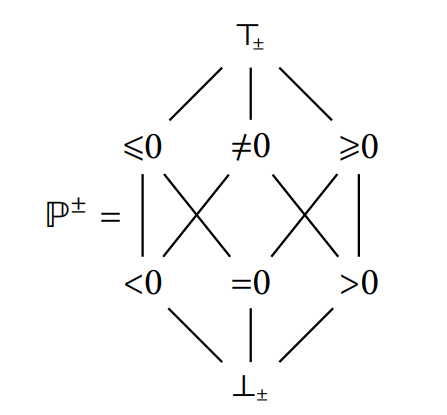
\includegraphics[scale=0.60]{content/images/static-analysis/sign1.png}
	
	\begin{itemize}
		\item result??: 
		\\ $\scriptsize in_{l_1}=in_{l_2}=in_{l_3}=in_{l_4}=\bot^{\mathcal{I}}$
		\\ $\scriptsize x_{l_4}^0 = ~[1,1] ;~~x_{l_4}^1 =~[1,2]~;~~x_{l_4}^2 =~[1,3]~;$
		\\ $\scriptsize x_{l_4}^3 = [1,4] ;...;~~x_{l_4}^k =~[1,k+1]~;$
		\item Intuition is that the result is $[1,\infty]$;
	\end{itemize}

\end{exampleblock}
\begin{exampleblock}{Widening examples:}
	$[1,1]~\nabla~[1,2]=[1,\infty] ~~~;~~~[1,3]~\nabla~[1,4]=[1,\infty]$\\
\end{exampleblock}
\end{frame}
\begin{frame}{Collecting Semantics for the $\mathcal{I}$ Domain with 1 Variable x and Widening}
\begin{itemize}
	\item  The $TF^{\scriptscriptstyle \mathcal{I}}_{\scriptscriptstyle \nabla}$ is defined as:\\$in_{li}=\sqcup(x_{pre_{li}})$ and $ x^k_{l_i}= x^{k-1}_{l_i}~~ \nabla~ TF^{\scriptscriptstyle \mathcal{I}}_{l_i}(in_{l_i}) ~\tiny \text{with} ~k>1,$\\ 
	$  TF^{\scriptscriptstyle \mathcal{I}}_{l_i}(in_{l_i}) =     \left\{ \begin{array}{rcl}
	\textstyle	in_{l_i} &  \mbox{\scriptsize if}& \textstyle l_i~\text{\scriptsize is}~while(B)~\mid~ if(B) ~\mid~;;   \\
	\textstyle	\|a\|_{li}^{\scriptscriptstyle \mathcal{I}}  & \mbox{\scriptsize if} & \textstyle l_i~\mbox{\scriptsize is}~x~=~a; \\
	\scriptstyle	\|a\|_{li}^{\scriptscriptstyle \mathcal{I}}~op_\mathcal{I}~ \|b\|_{li}^{\scriptscriptstyle \mathcal{I}}  & \mbox{\scriptsize if} &  \textstyle l_i~\mbox{\scriptsize is}~x~=~a~op_a~b; \\
	\dots & \mbox{if} & \dots
	\end{array}\right.$
	
	\item \scriptsize The abstract evaluation function:\\  $ \|a\|_{li}^ {\scriptscriptstyle \mathcal{I}} =     \left\{ \begin{array}{rcl}
	in_{l_i} & \mbox{ if}&  \text{x is a variable}   \\
	\gamma^{\scriptscriptstyle \mathcal{I}}(a)  & \mbox{ if} &  \text{x is a a constant value} 
	\end{array}\right.$
	
\end{itemize}
\begin{itemize}
	\item $\bot{\scriptscriptstyle \mathcal{I}} ~~op_{\scriptscriptstyle \mathcal{I}}~~ [a,b] = [a,b]~ op_{\scriptscriptstyle \mathcal{I}} ~\bot{\scriptscriptstyle \mathcal{I}} = ~\bot{\scriptscriptstyle \mathcal{I}}  $
	\item $[a,b] +_{\scriptscriptstyle \mathcal{I}}[c,d] = [a+c,b+d]$
	\item $[a,b] -_{\scriptscriptstyle \mathcal{I}}[c,d] = [a-d,b-c]$
	\item $ [a,b] \times_{\scriptscriptstyle \mathcal{I}}[c,d]=[min(B), max(B)] $\\ with $ B = \{(a \times c), (a \times d), (b\times c), (b \times d)\}$
\end{itemize}
\end{frame}


\begin{frame}{While Example in the  $\mathcal{I}$ Domain with Widening:}
\begin{exampleblock}{while loop:3}
	\centering   \tiny
  \usetikzlibrary{trees,shapes,decorations}
  \begin{tikzpicture}[%
    ->,
    >=stealth,
    node distance=0.3cm,
    noname/.style={%
      rectangle,
      minimum width=5em,
      minimum height=2em,
      draw
    }
  ]
    \node[noname] (1)                                             {[ x = 1; ] $l_1$};
    \node[noname] (2) [below=of 1]                                {[ while(??) ] $l_2$};
    \node[noname] (3) [below = 1cm of 2]                                {[ x = x+1; ] $l_3$};
    \node[noname] (4) [below right= 1cm of 2]                                {[ ;; ] $l_4$};
    
   
    

      \path 
   (1) edge                          node {} (2)
   (2) edge     [bend right=45pt]                     node  [yshift=5pt,right]{yes} (3)
   (2) edge                                         node  [yshift=5pt,right]{no} (4)
   (3) edge [bend right=45pt]                        node {} (2);
 
          
  \end{tikzpicture}
	\centering 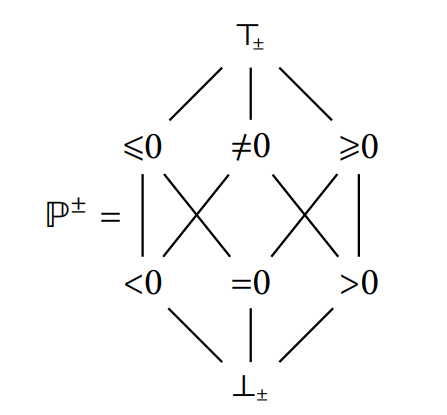
\includegraphics[scale=0.60]{content/images/static-analysis/sign1.png}
	\begin{itemize}
		\item result: 
		\\ $\scriptsize in_{l_1}=in_{l_2}=in_{l_3}=in_{l_4}=\bot^{\mathcal{I}}$
		\\ $\scriptsize x_{l_1}^0 = [1,1]~ ;~~x_{l_2}^0 =~[1,1]~;~~x_{l_3}^0 =~[2,2] ;~~x_{l_4}^0 =~[1,1]$
		\\ $\scriptsize x_{l_2}^1 = \bot^{\mathcal{I}}~ \nabla~[1,2] =~[1,2] ~; ~ x_{l_3}^2 =~\bot^{\mathcal{I}}~ \nabla~[3,3] = [3,3];$\\
		$\scriptsize x_{l_4}^1 =~ [1,1]~ \nabla[1,2]~= ~[1,\infty] $ *		
		\item Analysis Terminate;
		%		\item $\gamma_{I}([1, \infty])~=~\{x ~\in ~z~|~x \geq 1\} \equiv_\mathbb{Z}~~\{x ~\in ~z~|~x > 1\} = \gamma_\pm (Result ^\pm)$.
		%		\item Is the result going to be more precise for the same program by replacing $l_1$ with $x = 2$, $x = 3$;
		%		\item Is $TF^{\scriptscriptstyle \mathcal{I}}_{\scriptscriptstyle \nabla}$  in the interval domain always more precise than $TF^{\scriptscriptstyle \pm}$ 
	\end{itemize}
\end{exampleblock}
\end{frame}

\begin{frame}{While Example in the  $\mathcal{I}$ Domain with Widening:}
\begin{exampleblock}{while loop:3}
	\centering   \tiny
  \usetikzlibrary{trees,shapes,decorations}
  \begin{tikzpicture}[%
    ->,
    >=stealth,
    node distance=0.3cm,
    noname/.style={%
      rectangle,
      minimum width=5em,
      minimum height=2em,
      draw
    }
  ]
    \node[noname] (1)                                             {[ x = 1; ] $l_1$};
    \node[noname] (2) [below=of 1]                                {[ while(??) ] $l_2$};
    \node[noname] (3) [below = 1cm of 2]                                {[ x = x+1; ] $l_3$};
    \node[noname] (4) [below right= 1cm of 2]                                {[ ;; ] $l_4$};
    
   
    

      \path 
   (1) edge                          node {} (2)
   (2) edge     [bend right=45pt]                     node  [yshift=5pt,right]{yes} (3)
   (2) edge                                         node  [yshift=5pt,right]{no} (4)
   (3) edge [bend right=45pt]                        node {} (2);
 
          
  \end{tikzpicture}
	\centering 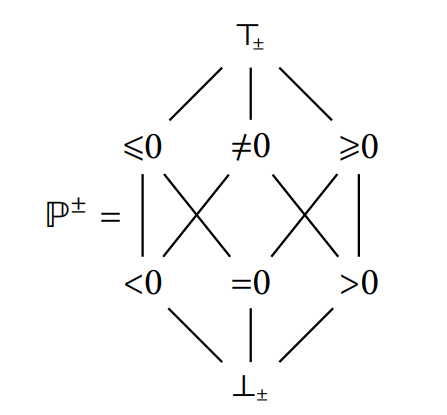
\includegraphics[scale=0.60]{content/images/static-analysis/sign1.png}
	\begin{itemize}
		\item result: 
		$ x_{l_4}^1 = [1,1] \nabla[1,2]= [1,\infty] $ 		
		\item Analysis Terminate;
				\item $\gamma_{I}([1, \infty])~=~\{x ~\in ~\mathbb{Z}~|~x \geq 1\} \equiv_\mathbb{Z}~~  \gamma_\pm (Result ^\pm)=  \{x ~\in~\mathbb{Z}~|~x > 0) )\}$.
				\item Is the result going to be more precise for the same program by replacing $l_1$ with $x = 2$; or $x = 3$;
				\item Is $TF^{\scriptscriptstyle \mathcal{I}}_{\scriptscriptstyle \nabla}$  in the interval domain always more precise than $TF^{\scriptscriptstyle \pm}$ 
	\end{itemize}
\end{exampleblock}
\end{frame}


\begin{frame}{Is Widening always converging in the right Way?}
\begin{exampleblock}{Another while loop}
	\centering   \tiny
  \usetikzlibrary{trees,shapes,decorations}
  \begin{tikzpicture}[%
    ->,
    >=stealth,
    node distance=0.3cm,
    noname/.style={%
      rectangle,
      minimum width=5em,
      minimum height=2em,
      draw
    }
  ]
    \node[noname] (1)                                             {[ x = 1; ] $l_1$};
    \node[noname] (2) [below=of 1]                                {[ while(??) ] $l_2$};
    \node[noname] (3) [below = 1cm of 2]                                {[ x = 0 ;] $l_3$};
    \node[noname] (4) [below right= 1cm of 2]                                {[ ;; ] $l_4$};
    
   
    

      \path 
   (1) edge                          node {} (2)
   (2) edge     [bend right=45pt]                     node  [yshift=5pt,right]{yes} (3)
   (2) edge                                         node  [yshift=5pt,right]{no} (4)
   (3) edge [bend right=45pt]                        node {} (2);
 
          
  \end{tikzpicture}
	\begin{itemize}
		\item Analyse this program using  $TF^{\scriptscriptstyle \pm}$, $TF^{\scriptscriptstyle \mathcal{I}}$ and $TF^{\scriptscriptstyle \mathcal{I}}_{\scriptscriptstyle \nabla}$
		\item Compare the result by concretization.
		\item Bonus question: do we need a widening operator for $TF^{\scriptscriptstyle \pm}$ and why?
		\item Propose a widening operator for $(\mathcal{P}_S(\mathbb{Z}), \subseteq)$.
		\end{itemize}
	\end{exampleblock}
\end{frame}



\begin{frame}{That complicated??}
\centering

\includegraphics[scale=0.60]{content/images/static-analysis/Abstractcousot.png}
\end{frame}


\begin{frame}{Just a symbols confusion}
\centering
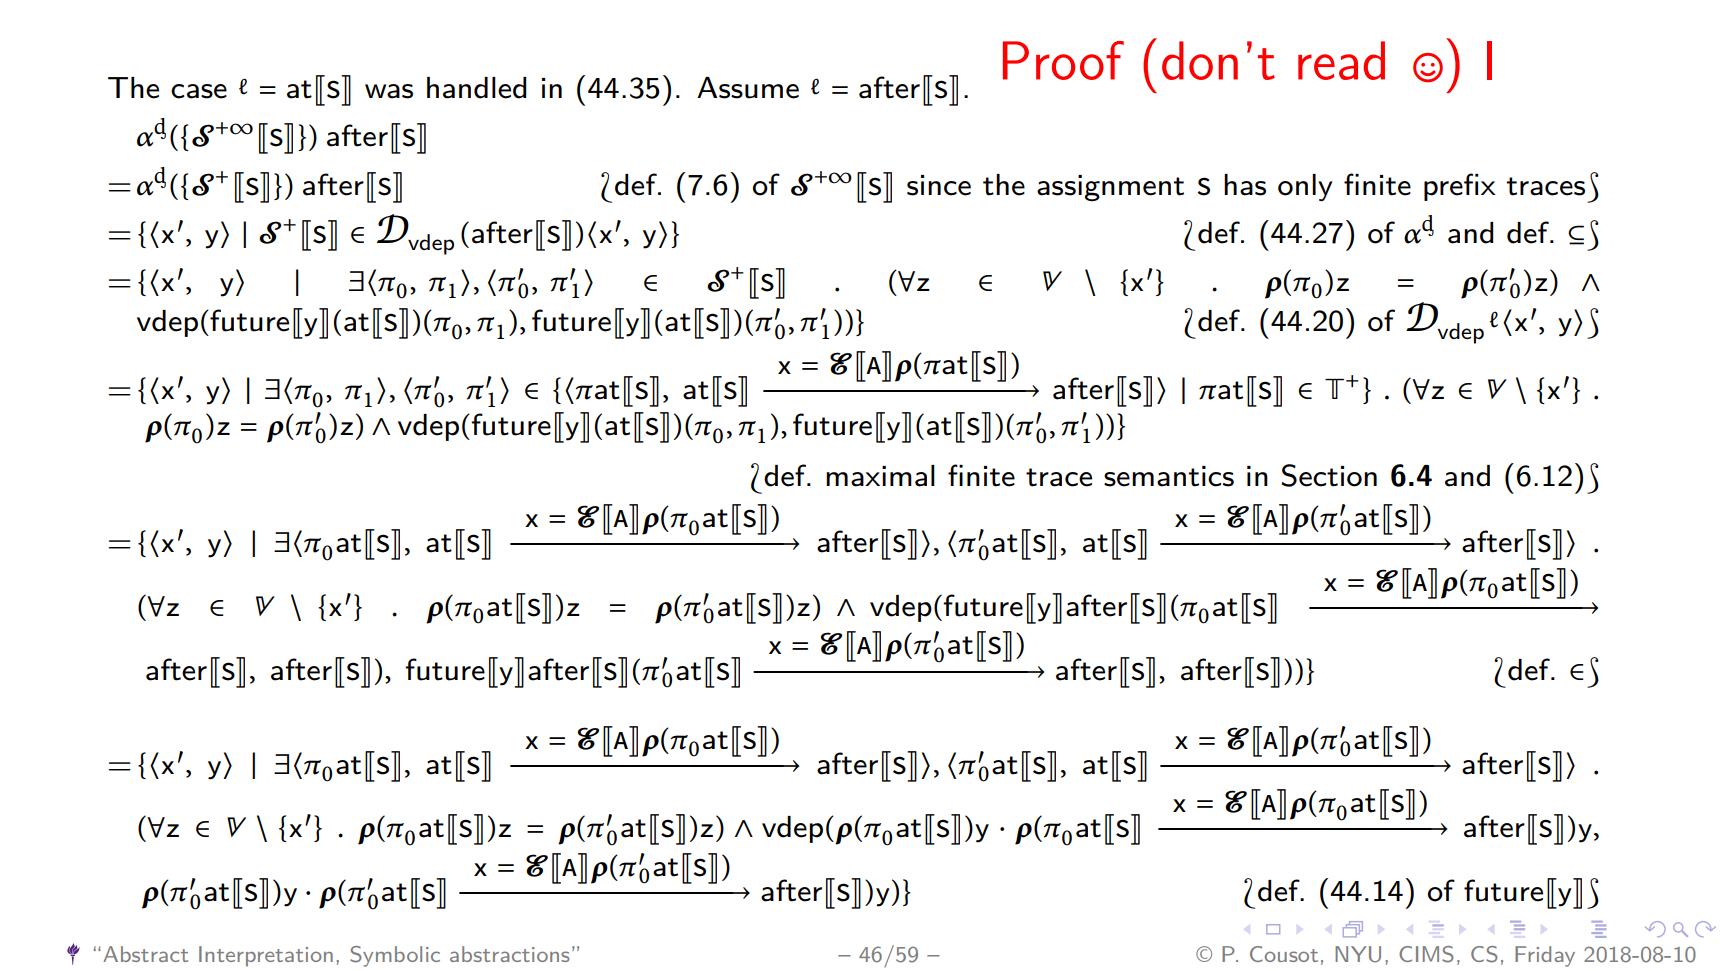
\includegraphics[scale=0.45]{content/images/static-analysis/abstractword.png}
\end{frame}

\begin{frame}{Framework for the $\mathcal{I}$ Domain with conditional Evaluation for 1 Variable and 1 Conditional:}
	
\scriptsize The transfer function with conditional evaluation $CTF_\mathcal{I}$ is defined as:\\ 
$ x_{l_i}= CTF^{\scriptscriptstyle \mathcal{I}}_{l_i}({\color{blue}in_{l_i}^b}),$ and \\ 
$ {\color{blue}in_{l_i}^b}= \sqcap (C(l_i) \sqcup(x_{pre_{li}})) ~\text{with}$\\

\xxx
$C(l_i)= \left\{ 
\begin{array}{lcr} {\color{blue}\alpha_{\scriptscriptstyle \mathcal{I}}^{\scriptscriptstyle b} (B)} & \mbox{\scriptsize if}& \textstyle while(B) \in \mbox{pred}(l_i)~ \mbox{and}~{\color{blue} yes~ branch} \\
{\color{blue}\alpha_{\scriptscriptstyle \mathcal{I}}^{\scriptscriptstyle b} (\neg B)} & \mbox{\scriptsize if}& \textstyle while(B) \in \mbox{pred}(l_i)~ \mbox{and}~{\color{blue} no~ branch} \\
\emptyset  & \mbox{\scriptsize otherwise} &  
\end{array}\right.$ \\

\xxx
$  CTF^{\scriptscriptstyle \mathcal{I}}_{l_i}(in_{l_i}) =     \left\{ \begin{array}{rcl}
\textstyle	in_{l_i} &  \mbox{\scriptsize if}& \textstyle l_i~\text{\scriptsize is}~while(B)~\mid~ if(B) ~\mid~;;   \\
\textstyle	\|a\|_{li}^{\scriptscriptstyle \mathcal{I}}  & \mbox{\scriptsize if} & \textstyle l_i~\mbox{\scriptsize is}~x~=~a; \\
\scriptstyle	\|a\|_{li}^{\scriptscriptstyle \mathcal{I}}~op_\mathcal{I}~ \|b\|_{li}^{\scriptscriptstyle \mathcal{I}}  & \mbox{\scriptsize if} &  \textstyle l_i~\mbox{\scriptsize is}~x~=~a~op_a~b; \\
\dots & \mbox{if} & \dots
\end{array}\right.$
\newline

\xxx
pred$(l_i)$ is the set of predecessors of $l_i$.\\
Computing $C(li)$  for $if(B)$ is the same as for $While(B)$.

\end{frame}

\begin{frame}{While loop with Conditional}
\begin{exampleblock}{Without widening $CTF_\mathcal{I}$}
  \centering   \tiny
  \usetikzlibrary{trees,shapes,decorations}
  \begin{tikzpicture}[%
    ->,
    >=stealth,
    node distance=0.3cm,
    noname/.style={%
      rectangle,
      minimum width=5em,
      minimum height=2em,
      draw
    }
  ]
    \node[noname] (1)                                             {[ x = 1; ] $l_1$};
    \node[noname] (2) [below=of 1]                                {[ while(x < 1001) ] $l_2$};
    \node[noname] (3) [below = 1cm of 2]                                {[ x = x + 1 ;] $l_3$};
    \node[noname] (4) [below right= 1cm of 2]                                {[ ;; ] $l_4$};
    
   
    

      \path 
   (1) edge                          node {} (2)
   (2) edge     [bend right=45pt]                     node  [yshift=5pt,right]{yes} (3)
   (2) edge                                         node  [yshift=5pt,right]{no} (4)
   (3) edge [bend right=45pt]                        node {} (2);
 
          
  \end{tikzpicture}
		\begin{itemize}
		\item $\alpha_{\scriptscriptstyle \mathcal{I}}^{\scriptscriptstyle b} ( x < 1001) = [-\infty,1000]$
		\item $\alpha_{\scriptscriptstyle \mathcal{I}}^{\scriptscriptstyle b} ( x \geq 1001) = [1001,\infty]$
		\item $x_{l_1}~=~ [1,1]$ and  $x_{l_2}~=~ \sqcup(x_{l_1},x_{l_3})$
		\item $x_{l_3}~=~ \sqcap(x_{l_2},[-\infty,1000]~) +_\mathcal{I} [1,1]$ and  $x_{l_4} =~\sqcap(x_{l_2},[1001,\infty] $
		\item initialization:
		\item $x_{l_1}^0=~ [1,1]$  and $x_{l_2}^0~=~ [1,1]$\\
		\item $x_{l_3}^0=~ \sqcap([1,1],[-\infty,1000]) ~+_\mathcal{I}~ [1,1] = [2,2]$  and $x_{l_4}^0~=~ \sqcap([1,1],[1001,\infty]) =\emptyset $\\
		\item first iteration:
		\item $x_{l_1}^1=~ [1,1]= ??~~$  and $~~~~x_{l_2}^1~=\sqcup([1,1],[2,2])~=~??$\\
		\item $x_{l_3}^1=~ (\sqcap(x_{l_2}^1,[-\infty,1000]) +_\mathcal{I} ~[1,1]) ~= ~??$  and $x_{l_4}^1~=~ \sqcap(x_{l_2}^1,[1001,\infty]) = ?? $\\
	\end{itemize}
\end{exampleblock}
\end{frame}

\begin{frame}{Framework for the $\mathcal{I}$ Domain with conditional Evaluation for 1 Variable and 1 Conditional and Widening:}
\scriptsize The transfer with conditional evaluation $CTF_\mathcal{I}^\nabla$ is defined as:\\ ${\color{blue} x_{l_i}^k=  x_{l_i}^{k-1}~\nabla~ CTF^{\scriptscriptstyle \mathcal{I}}_{l_i}(in_{l_i}^b})$ for $k > 1$ and \\ $ {\color{blue}in_{l_i}^b}= \sqcap (C \sqcup(x_{pre_{li}})) ~\text{with}$

\xxx
$C(l_i)= \left\{ 
\begin{array}{lcr} {\color{blue}\alpha_{\scriptscriptstyle \mathcal{I}}^{\scriptscriptstyle b} (B)} & \mbox{\scriptsize if}& \textstyle ~while(B) \in \mbox{pred}(l_i)~ \mbox{and}~{\color{blue} yes~ branch} \\
	
	{\color{blue}\alpha_{\scriptscriptstyle \mathcal{I}}^{\scriptscriptstyle b} (\neg B)} & \mbox{\scriptsize if}& \textstyle while(B) \in \mbox{pred}(l_i)~ \mbox{and}~{\color{blue} no~ branch} \\
	\emptyset  & \mbox{\scriptsize otherwise} &  
\end{array}\right.$ \\

\xxx
$  CTF^{\scriptscriptstyle \mathcal{I}}_{l_i}(in_{l_i}) =     \left\{ \begin{array}{rcl}
	\textstyle	in_{l_i} &  \mbox{\scriptsize if}& \textstyle l_i~\text{\scriptsize is}~while(B)~\mid~ if(B) ~\mid~;;   \\
	\textstyle	\|a\|_{li}^{\scriptscriptstyle \mathcal{I}}  & \mbox{\scriptsize if} & \textstyle l_i~\mbox{\scriptsize is}~x~=~a; \\
	\scriptstyle	\|a\|_{li}^{\scriptscriptstyle \mathcal{I}}~op_\mathcal{I}~ \|b\|_{li}^{\scriptscriptstyle \mathcal{I}}  & \mbox{\scriptsize if} &  \textstyle l_i~\mbox{\scriptsize is}~x~=~a~op_a~b; \\
	\dots & \mbox{if} & \dots
\end{array}\right.$
\newline

\xxx
pred$(l_i)$ is the set of predecessors of $l_i$.\\
Computing $C(li)$  for $if(B)$ is the same as for $While(B)$.

\end{frame}




\begin{frame}{While loop with Boolean}
\begin{exampleblock}{While loop with widening $CTF_\mathcal{I}^\nabla$}
	\centering   \tiny
  \usetikzlibrary{trees,shapes,decorations}
  \begin{tikzpicture}[%
    ->,
    >=stealth,
    node distance=0.3cm,
    noname/.style={%
      rectangle,
      minimum width=5em,
      minimum height=2em,
      draw
    }
  ]
    \node[noname] (1)                                             {[ x = 1; ] $l_1$};
    \node[noname] (2) [below=of 1]                                {[ while(x < 1001) ] $l_2$};
    \node[noname] (3) [below = 1cm of 2]                                {[ x = x + 1 ;] $l_3$};
    \node[noname] (4) [below right= 1cm of 2]                                {[ ;; ] $l_4$};
    
   
    

      \path 
   (1) edge                          node {} (2)
   (2) edge     [bend right=45pt]                     node  [yshift=5pt,right]{yes} (3)
   (2) edge                                         node  [yshift=5pt,right]{no} (4)
   (3) edge [bend right=45pt]                        node {} (2);
 
          
  \end{tikzpicture}
	\begin{itemize}
		\item $\alpha_{\scriptscriptstyle \mathcal{I}}^{\scriptscriptstyle b} ( x < 1001) = [-\infty,1000]$
		\item $\alpha_{\scriptscriptstyle \mathcal{I}}^{\scriptscriptstyle b} ( x \geq 1001) = [1001,\infty]$
		\item $x_{l_1}~=~ [1,1]$ and  $x_{l_2}~=~ \sqcup(x_{l_1},x_{l_3})$
		\item $x_{l_3}~=~ \sqcap(x_{l_2},[-\infty,1000]~) +_\mathcal{I} [1,1]$ and  $x_{l_4} =~\sqcap(x_{l_2},[1001,\infty] $
		\item initialization:
		\item $x_{l_1}^0=~ [1,1]$  and $x_{l_2}^0~=~ [1,1]$\\
		\item $x_{l_3}^0=~ \sqcap([1,1],[-\infty,1000]) ~+_\mathcal{I}~ [1,1] = [2,2]$  and $x_{l_4}^0~=~ \sqcap([1,1],[1001,\infty]) =\emptyset $\\
	    \item first iteration:
	    \item $x_{l_1}^1=~ [1,1]~\nabla~[1,1]= ??~~~~$  and $~~~~x_{l_2}^1~=~ [1,1]~\nabla~\sqcup([1,1],[2,2])~=~??$\\
	    \item $x_{l_3}^1=~ [2,2]~\nabla~(\sqcap(x_{l_2}^1,[-\infty,1000]) +_\mathcal{I} ~[1,1]) ~= ~??$  and $x_{l_4}^1~=~ \bot_\mathcal{I}~\nabla~\sqcap(x_{l_2}^1,[1001,\infty]) = ?? $\\	
	\end{itemize}
\end{exampleblock}
\end{frame}

\begin{frame}{While loop with Boolean}
\begin{exampleblock}{While loop with widening $CTF_\mathcal{I}^\nabla$}
	\centering   \tiny
  \usetikzlibrary{trees,shapes,decorations}
  \begin{tikzpicture}[%
    ->,
    >=stealth,
    node distance=0.3cm,
    noname/.style={%
      rectangle,
      minimum width=5em,
      minimum height=2em,
      draw
    }
  ]
    \node[noname] (1)                                             {[ x = 1; ] $l_1$};
    \node[noname] (2) [below=of 1]                                {[ while(x < 1001) ] $l_2$};
    \node[noname] (3) [below = 1cm of 2]                                {[ x = x + 1 ;] $l_3$};
    \node[noname] (4) [below right= 1cm of 2]                                {[ ;; ] $l_4$};
    
   
    

      \path 
   (1) edge                          node {} (2)
   (2) edge     [bend right=45pt]                     node  [yshift=5pt,right]{yes} (3)
   (2) edge                                         node  [yshift=5pt,right]{no} (4)
   (3) edge [bend right=45pt]                        node {} (2);
 
          
  \end{tikzpicture}
	\begin{itemize}
		\item the $CTF_\mathcal{I}^\nabla$ in few iterations, faster than $CTF_\mathcal{I}$:
	\item the $CTF_\mathcal{I}^\nabla$ results are $x_{l_3,\nabla}^2=~[2,\infty] $  and $x_{l_4,\nabla}^3~=~[1001, \infty] $\\	
\item the $CTF_\mathcal{I}$ results are $x_{l_3}^{999}=~[2,1001] $  and $x_{l_4}^{1000}~=~[1001,1001] $\\
\item the $\nabla$ outruns the while conditional, the result is a medium fixpoint.
		\item Can we use $\nabla$ in a different location of TF??
		\item there is no good position.
		\item the solution is the interpolate using \color{blue}{narrowing $\vartriangle$}.  
	\end{itemize}
\end{exampleblock}
\end{frame}


\begin{frame}{Narrowing: Fixpoint Accelerator Fixator}
\begin{itemize}
	\item The $\vartriangle I$  for intervals is defined as : $\nabla : \mathcal{I} \times \mathcal{I} \rightarrow \mathcal{I}$\\
	\begin{enumerate}
		\item $[a,b] ~\vartriangle ~\bot_\mathcal{I}= ~\bot_\mathcal{I} ~\vartriangle~ [a,b]~ = ~[a,b]  $
		\item$[a,b] ~\vartriangle ~[c,d]= [l,r]$ such as : \\   
		$	\left\{ \begin{array}{l}
		l = \{ \begin{array}{l c r} a & \mbox{if} & a \neq -\infty
		\\  c & \mbox{otherwise} &  \end{array}\\
		r = \{ \begin{array}{l c r} b & \mbox{if} & b \neq \infty
		\\  d & \mbox{otherwise} & \\ \end{array}\\
		\end{array}\right.$
	\end{enumerate}
	
\end{itemize}		
\end{frame}


\begin{frame}{Narrowing: How to use it?}
\begin{itemize}
	\item Use it downward :after reaching a  fixpoint $\phi^k$.
	\item Does not always recover the least fixpoint .
	\item initialization: $\bar{\phi}^0 = \phi^k$.
	\item Iteration: $\bar{\phi}^k~=~\bar{\phi}^{(k-1)} \vartriangle TF(\bar{\phi}^{(k-1)}).$ 
	\item Does not always terminate.
	
\end{itemize}	 
\end{frame}



\begin{frame}{While loop with Boolean Narrowing and Widening}
\begin{exampleblock}{While loop with widening and narrowing $CTF_\mathcal{I}^\nabla$}
	\centering   \tiny
  \usetikzlibrary{trees,shapes,decorations}
  \begin{tikzpicture}[%
    ->,
    >=stealth,
    node distance=0.3cm,
    noname/.style={%
      rectangle,
      minimum width=5em,
      minimum height=2em,
      draw
    }
  ]
    \node[noname] (1)                                             {[ x = 1; ] $l_1$};
    \node[noname] (2) [below=of 1]                                {[ while(x < 1001) ] $l_2$};
    \node[noname] (3) [below = 1cm of 2]                                {[ x = x + 1 ;] $l_3$};
    \node[noname] (4) [below right= 1cm of 2]                                {[ ;; ] $l_4$};
    
   
    

      \path 
   (1) edge                          node {} (2)
   (2) edge     [bend right=45pt]                     node  [yshift=5pt,right]{yes} (3)
   (2) edge                                         node  [yshift=5pt,right]{no} (4)
   (3) edge [bend right=45pt]                        node {} (2);
 
          
  \end{tikzpicture}
	\begin{itemize}
		\item $\alpha_{\scriptscriptstyle \mathcal{I}}^{\scriptscriptstyle b} ( x < 1001) = [-\infty,1000]$
		\item $\alpha_{\scriptscriptstyle \mathcal{I}}^{\scriptscriptstyle b} ( x \geq 1001) = [1001,\infty]$
		\item $x_{l_1}~=~ [1,1]$ and  $x_{l_2}~=~ \sqcup(x_{l_1},x_{l_3})$
		\item $x_{l_3}~=~ \sqcap(x_{l_2},[-\infty,1000]~) +_\mathcal{I} [1,1]$ and  $x_{l_4} =~\sqcap(x_{l_2},[1001,\infty] $
		
		\item After widening iterations:\\
		\item $x_{l_3}^4~ =~[2,\infty] $ and $x_{l_4}^4~=~[1001,\infty]  $\\
		\item  narrowing initialization:\\
		\item $\overline{x}_{l_3}^0 = x_{l_3}^4~ =~[2,\infty] $ and $\overline{x}_{l_4}^0=x_{l_4}^4~=~[1001,\infty]  $\\
		\item  narrowing initialization:\\
		\item $\overline{x}_{l_3}^1~= \overline{x}_{l_3}^0  \vartriangle TF_\mathcal{I}(\overline{x}_{l_3}^0)~=~ [2,1001]$ and $\overline{x}_{l_4}^1= \overline{x}_{l_4}^0 \vartriangle TF_\mathcal{I}(\overline{x}_{l_4}^0) =[1001,1001] $\\	
	\end{itemize}
\end{exampleblock}
\end{frame}

\begin{frame}{Narrowing: How to use it?}
\begin{itemize}
	\item Use it downward:after reaching a suspicious fixpoint $\phi^k$.
	\item Does not always recover the least fixpoint .
	\item initialization: $\bar{\phi}^0 = \phi^k$.
	\item Iteration: $\bar{\phi}^k~=~\bar{\phi}^{k-1} \vartriangle TF(\bar{\phi^0}).$ 
	\item Does not always terminate. But why??
	\end{itemize}
\centering 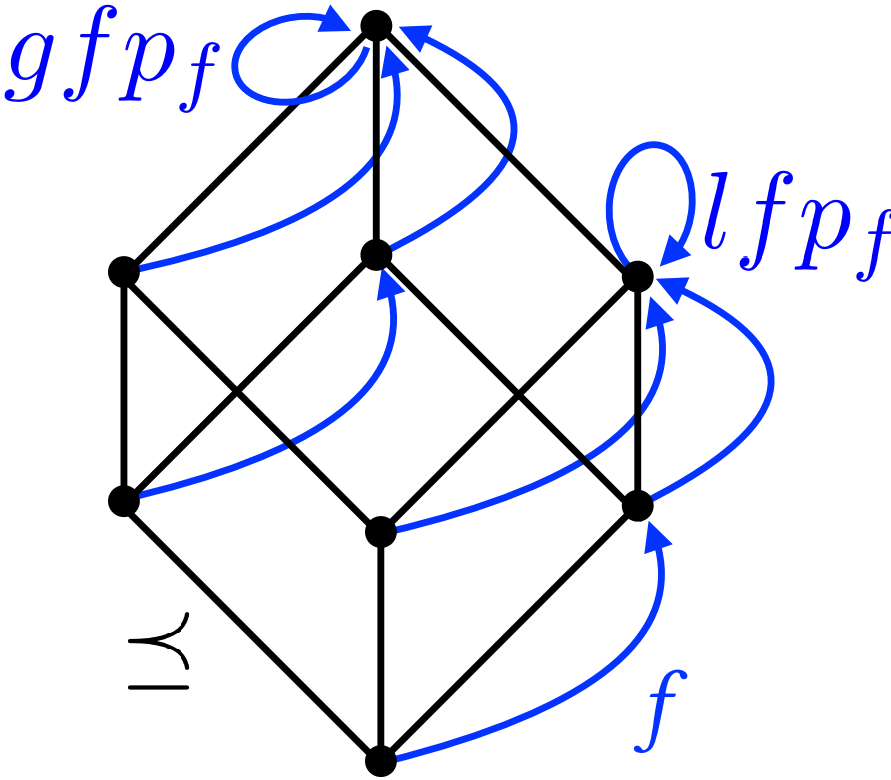
\includegraphics[scale=0.25]{content/images/static-analysis/lfp.png}
\end{frame}


\begin{frame}{Did you get it??}
\centering 
\includegraphics[scale=0.25]{content/images/static-analysis/overcome.jpg}
\end{frame}


\begin{frame}{Informal Wrap Up: How to design Abstract Interpretation Program Analysis}
\begin{enumerate}
	\item Choose/invent \textcolor{blue}{abstract domains}, design the $\gamma$ and $\alpha$ and map to the concrete domain of the program. (Mathematical theories).
	\item Define \textcolor{blue}{arithmetic and Boolean  basic operation} related to the abstract domain:  (Implement)
	\item Define  \textcolor{blue}{TF} (abstract data-analysis framework). (Implement)
	\item For every step, proof \textcolor{blue}{soundness and termination}, (formal proofs).
	\item Experiment and adapt by \textcolor{blue}{tuning the transfer functions} for precision or convergence by: 
	\begin{itemize}
		\item Introduce operators such as: $\nabla$ and  $\vartriangle$ ...
		\item Compose new $TF$ using those operators where, when, how long?
	\end{itemize}
	\end{enumerate}
\end{frame}

\begin{frame}{Informal Wrap Up: How to interpret the analysis results in Abstract interpretation}
\begin{itemize}
	\item When using one \textbf{Sound} Abstract framework:
	\begin{enumerate}
		\item if the result is : ok $\Rightarrow$ Verdict is: \textcolor{green}{The program is safe}.
		\item if the answer is : error $\Rightarrow$ ??
	\end{enumerate}	

\end{itemize}
\end{frame}

\begin{frame}{Informal Wrap Up: How to interpret the analysis results in Abstract interpretation}
\begin{itemize}
	\item When using one \textbf{Sound} Abstract framework for detecting bad states:
	\begin{enumerate}
		\item if the result is : ok $\Rightarrow$ Verdict is: \textcolor{green}{ The program is safe}.
		\item if the answer is : error $\Rightarrow$ Verdict is: \textcolor{orange}{Inconclusive} (maybe a false alarm)
	\end{enumerate}	
	\item When using  Multiple \textbf{Sound} frameworks:
\begin{enumerate}
	\item If \textbf{all} frameworks says: false $\Rightarrow$ Verdict is: ??
	\item If \textbf{one} framework answers: ok  $\Rightarrow$ Verdict is: ??
\end{enumerate}	
	
\end{itemize}
\end{frame}


\begin{frame}{Numerical domains :}
\centering 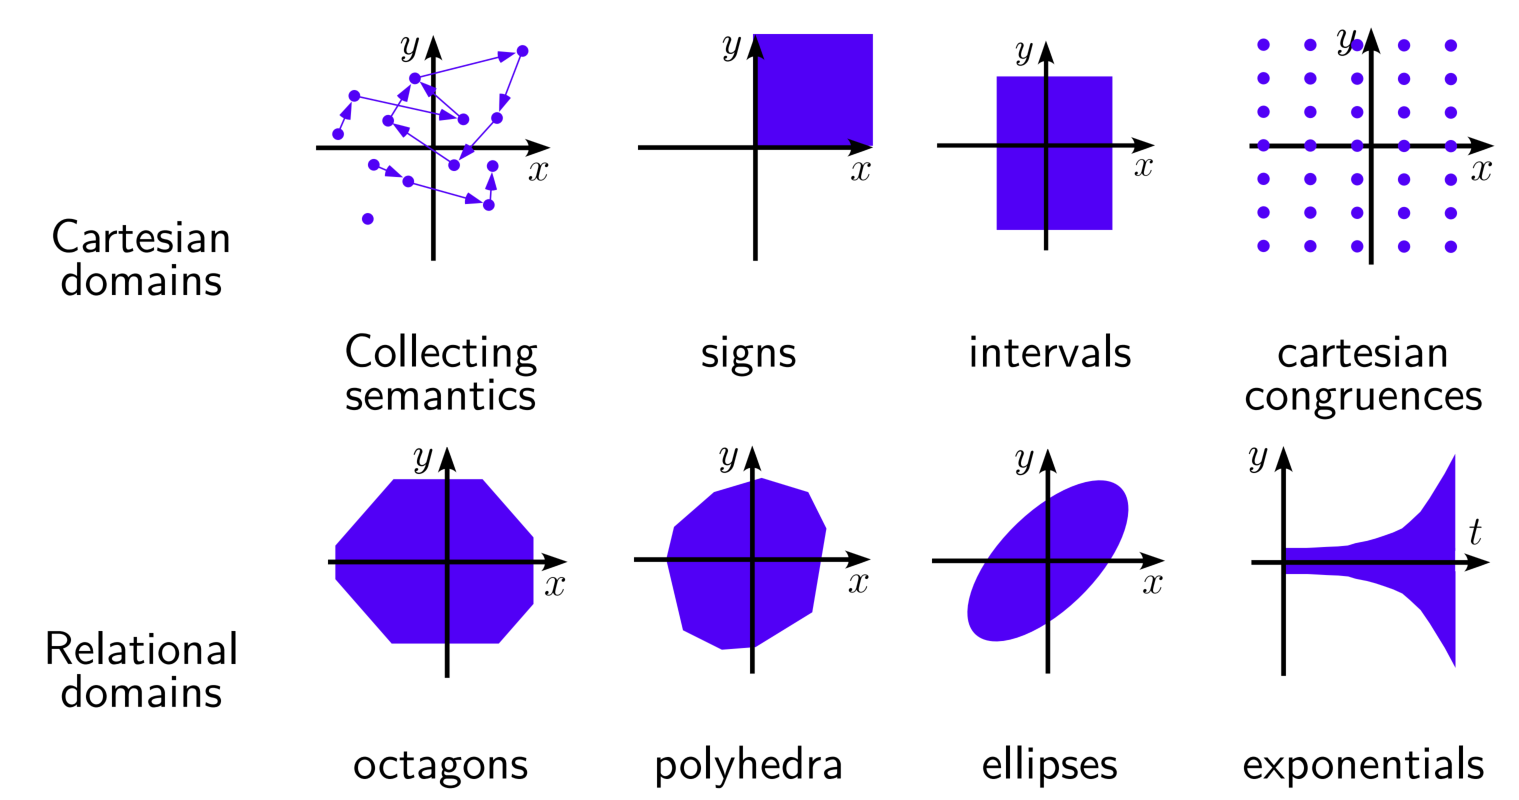
\includegraphics[scale=0.45]{content/images/static-analysis/domains.png}
\end{frame}

\begin{frame}{Domains are composable :}
\begin{theorem}[Composition of Galois connections:]
	let $(\mathcal{C}, \preceq_c) \galois{\alpha_1}{\gamma_1} (\mathcal{A}_1, \preceq_{a_1})$ and $(\mathcal{A}_1, \preceq_{c_1}) \galois{\alpha_2}{\gamma_2} (\mathcal{A}_2, \preceq_{a_2})$ then:\\
	$(\mathcal{C}, \preceq_c) \galois{\color{blue}{\alpha_2 \comp \alpha_1}}{\color{blue}{\gamma_1 \comp \gamma_2}} (\mathcal{A}_2, \preceq_{a_2})$.
\end{theorem}
\end{frame}


\begin{frame}{Industrial Applications:}
\begin{itemize}
	\item How is abstract interpretation used for safety critical systems.
	\item We used a mini-imperative language with one type: $\mathbb{Z}$.
	\item We used simple examples on simple domains.
\end{itemize}
\end{frame}

\begin{frame}{Programming Languages:}
\begin{itemize}
	\item We used a mini-imperative language with one type.
	\item No pointers.
	\item The concrete domain was $(\mathcal{P_S}(\mathbb{Z}),\subseteq)$.
	\item Not the case for "real" programming language.
	\item Is it better or worse??
	\end{itemize}
\end{frame}

\begin{frame}{Programming Languages: $Types 1~\subset~\mathbb{Z}$}
\centering 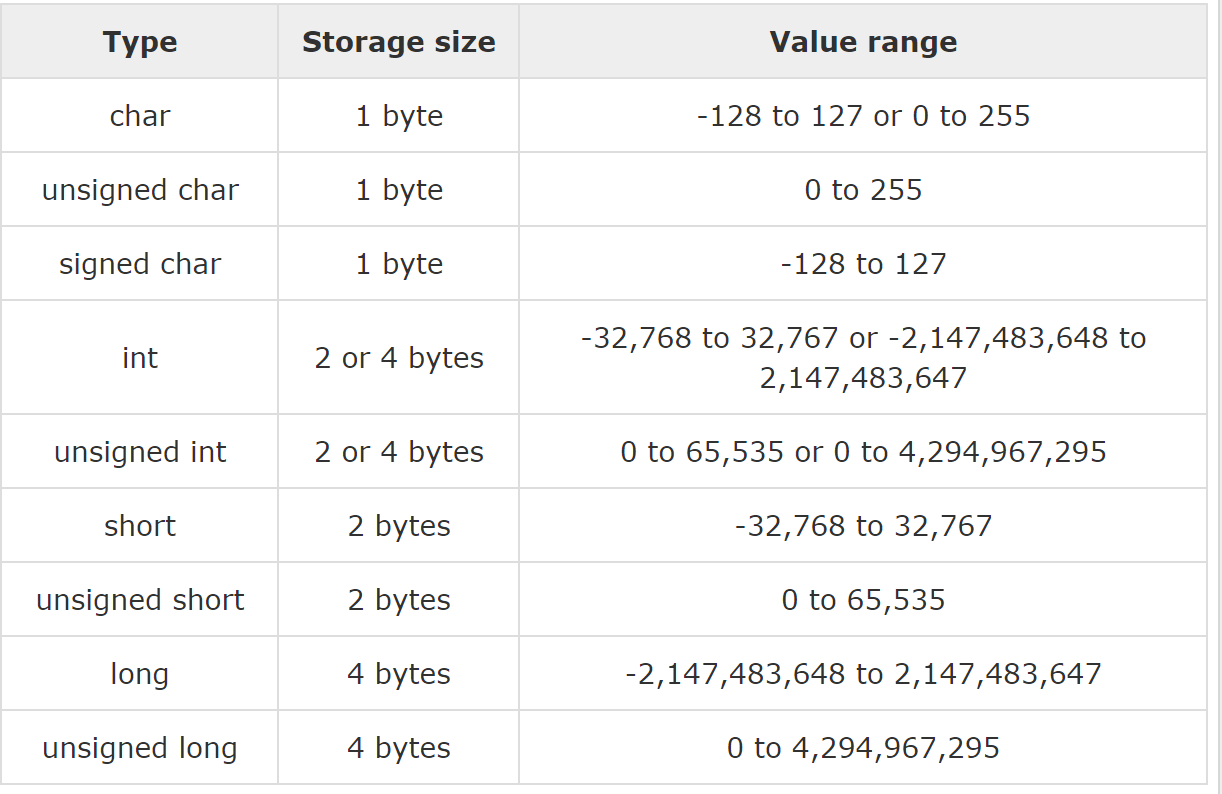
\includegraphics[scale=0.45]{content/images/static-analysis/int.png}
\end{frame}


\begin{frame}{Programming Languages: $Types~2~\subset~\mathbb{R}$}
	\centering 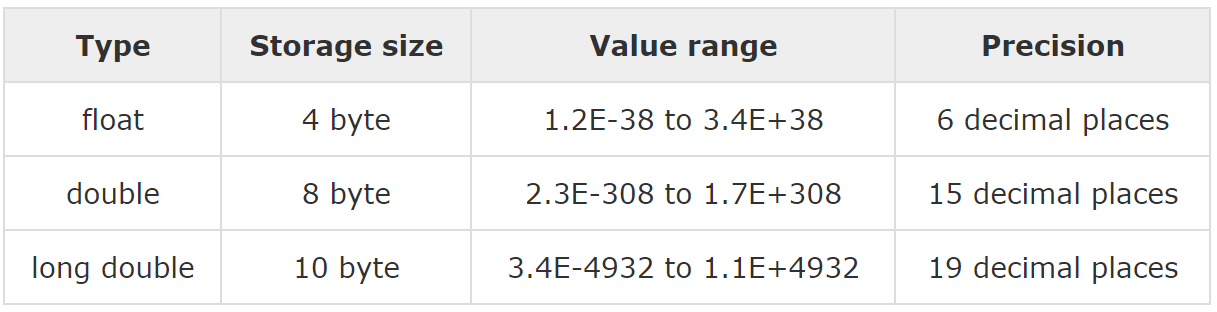
\includegraphics[scale=0.45]{content/images/static-analysis/RR.png}
     
	\xxx
    \centering 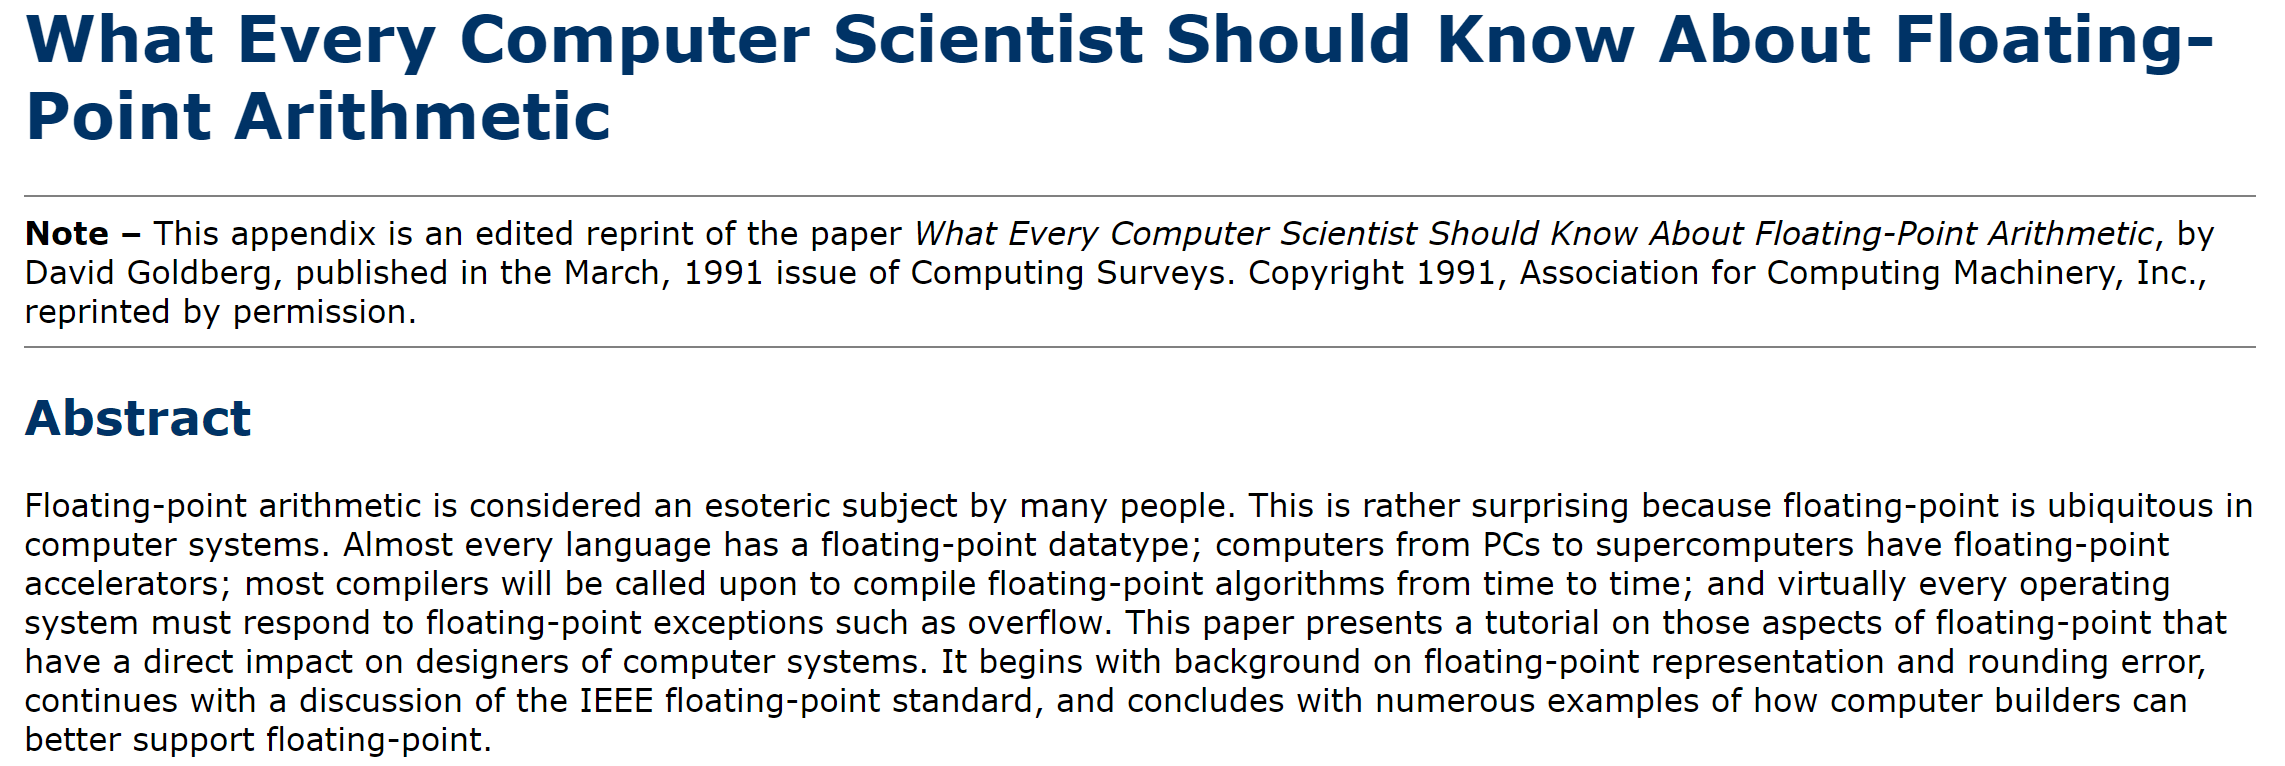
\includegraphics[scale=0.3]{content/images/static-analysis/floating.png}
\end{frame}


\begin{frame}{Runtime Errors are a perfect Match for Numerical Abstract Interpretation}
	\begin{itemize}
		\item Division by zero.
		\item Type overflows. ($int~z= Int_{max} + 1$)
		\item Array overflows. ($a[i] ~ where~ i> size(a)$);
		\item ...
	\end{itemize}
    \lstinputlisting[language=C, basicstyle =\tiny]{content/images/static-analysis/overflow.txt}
\end{frame}


\begin{frame}{Tools}
\centering 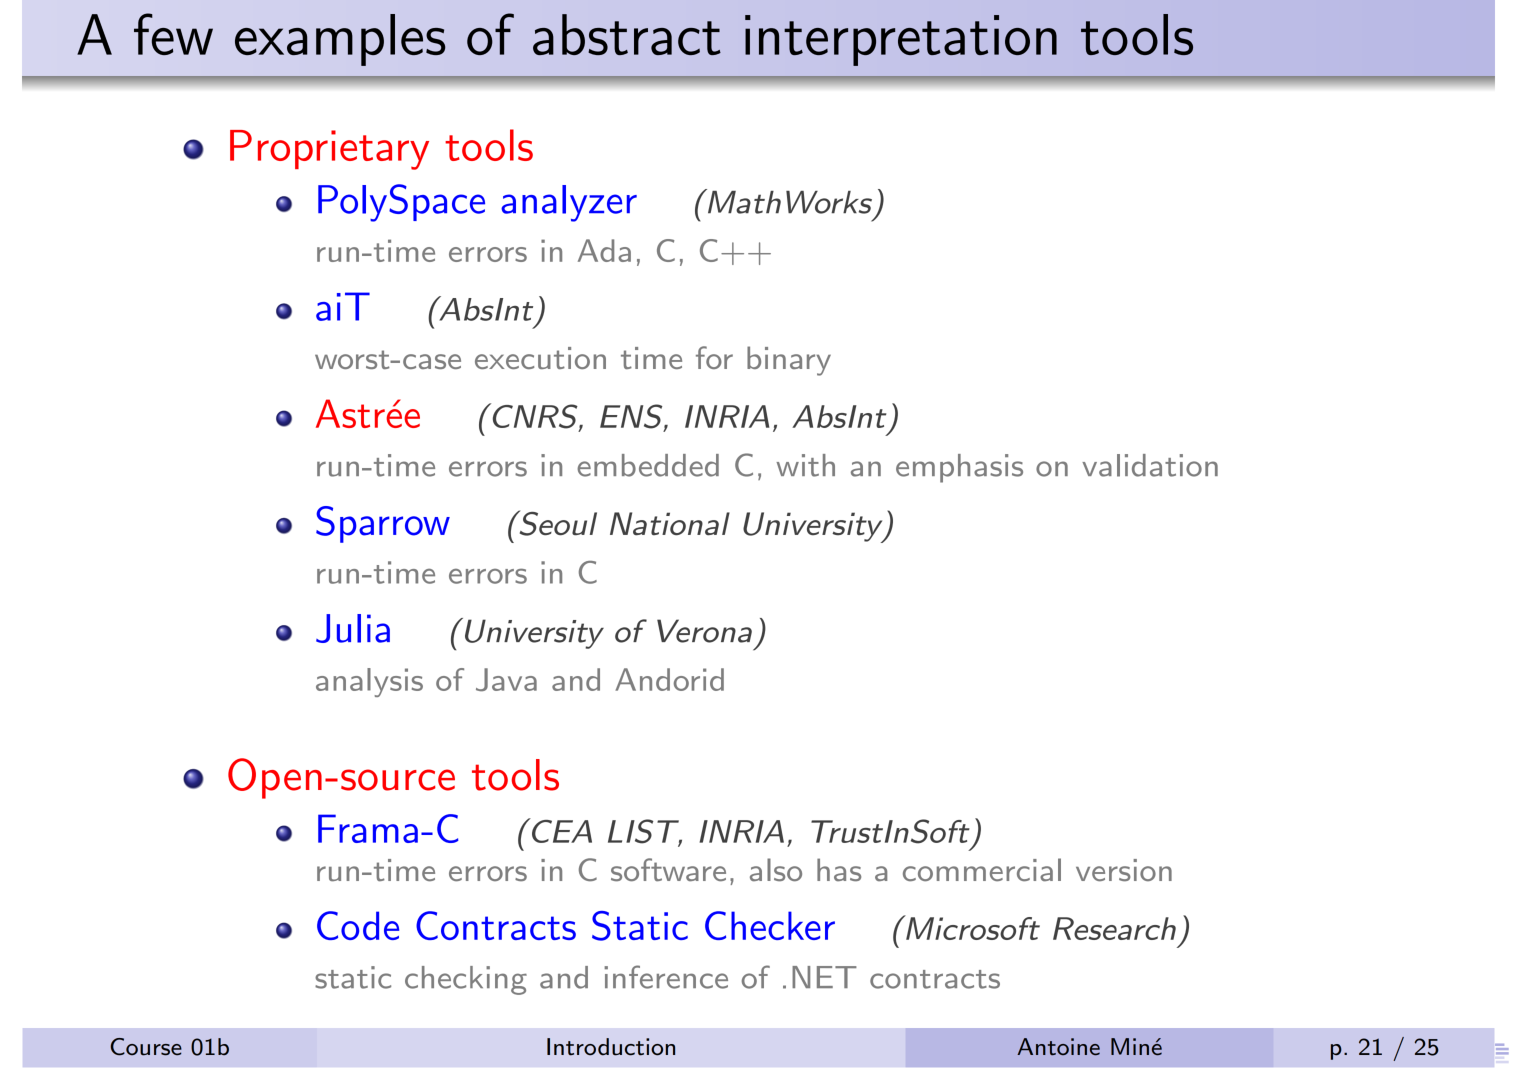
\includegraphics[scale=0.45]{content/images/static-analysis/tools.png}
\end{frame}

\begin{frame}{Tools}
\centering 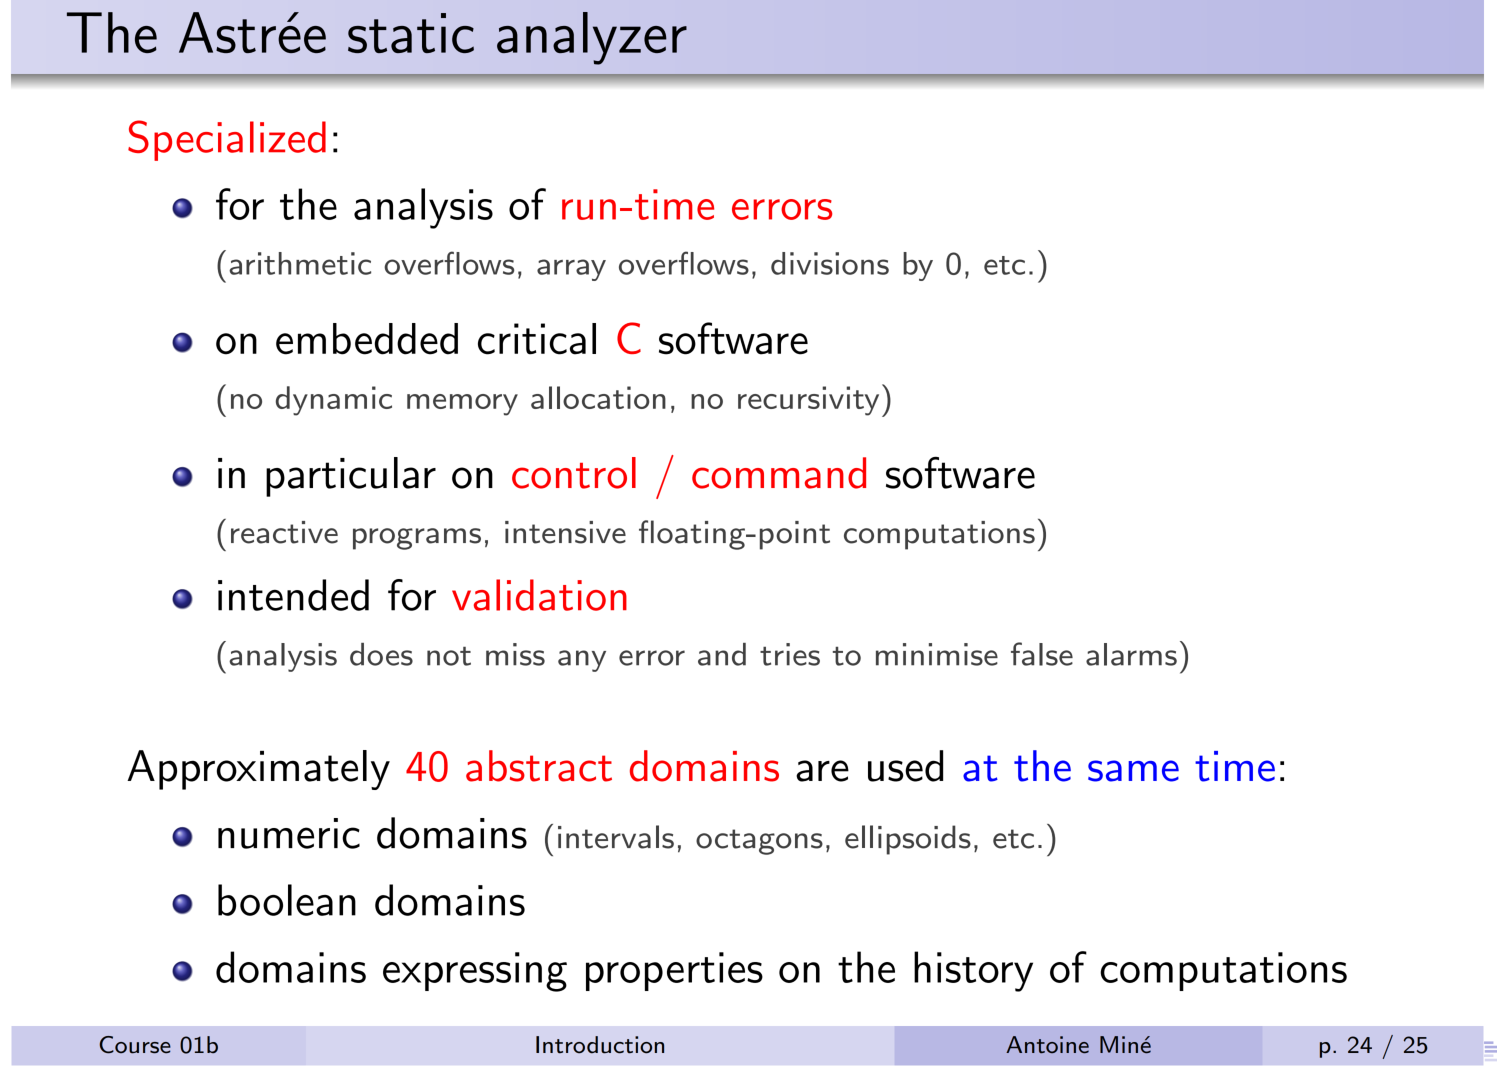
\includegraphics[scale=0.45]{content/images/static-analysis/astree.png}
\end{frame}


\begin{frame}{Results}
\centering 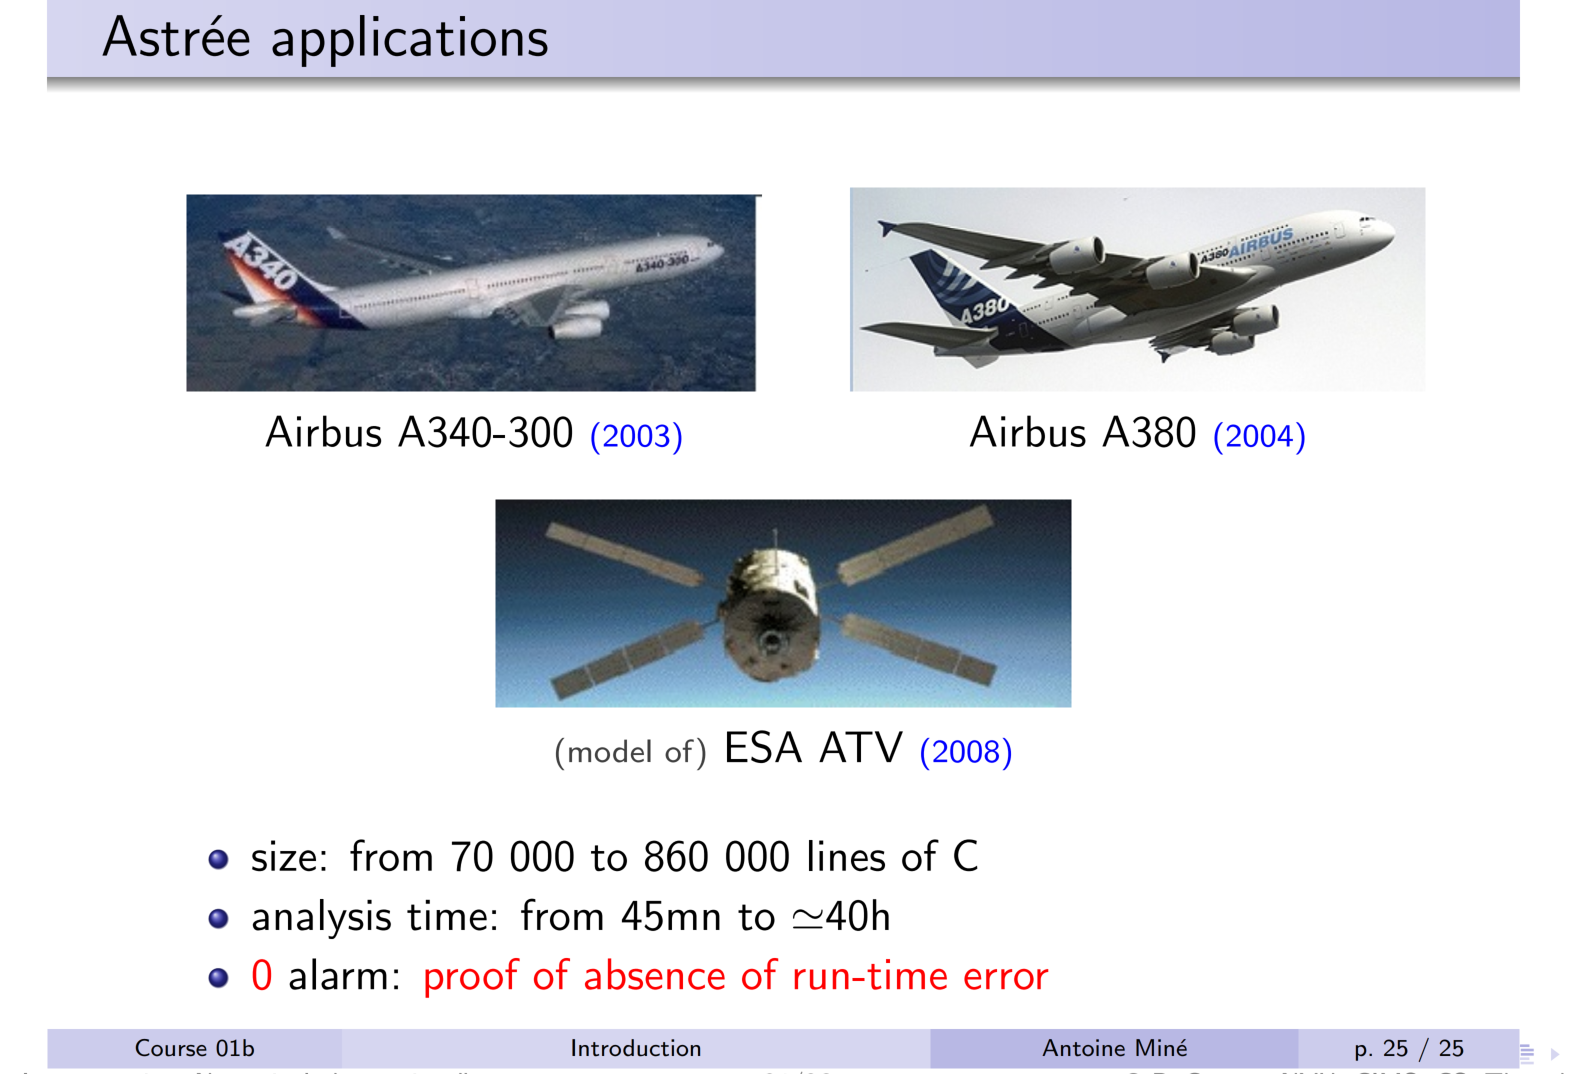
\includegraphics[scale=0.45]{content/images/static-analysis/astreresult.png}
\end{frame}

\section{Deductive verification}


\begin{frame}{Deductive verification}
\footnotesize
\begin{tabular}{|c|c|}
	\hline
	Syntactic & Semantic\\
	\hline 
	$P$ has n statements &  $P$ terminates\\
	
	$P_1 =_{syn} P_2$  & $\forall x.P_1(x) = P_2(x)$\\
	$P$ contains n program functions &  $\color{blue}{P \equiv  f}$ ($f$ a mathematical function)\\
	\hline
\end{tabular}
\end{frame}

\begin{frame}{Where are we now?}
\begin{itemize}
	\item Back to \textcolor{blue}{Static Program Analysis}.
	\item Plus some notions of \textcolor{blue}{Theorem Proving}.
	\item Introducing the notion of \textcolor{blue}{Contracts for Programs}.
\end{itemize}
\end{frame}

\begin{frame}{Research background}
\begin{itemize}\setlength\itemsep{1em}
	\item R. W. Floyd. 
 \textcolor{blue}{Assigning Meanings to Programs.}\\ 	Proc. of Symposia in Applied Mathematics, 1967.
	\item C. A. R. (Tony) Hoare.\\ \textcolor{blue}{An Axiomatic Basis for Computer Programming.}\\ Communications of the ACM, 1969.
	\item E. W. Dijkstra. \textcolor{blue}{A Discipline of Programming}.\\ Prentice Hall, 1976.
	\begin{itemize}
		\item "Program testing can be used to show the presence of bugs, but never to show their absence! "
		\item "Simplicity is a great virtue but it requires hard work to achieve it and education to appreciate it."
	\end{itemize}
	\pause
	\item P.Cousot \& R.Cousot.\\ \textcolor{blue}{Abstract interpretation: a unified lattice model for static analysis of programs by construction or approximation of fixpoints}. \\ Principles of programming languages. ACM, 1977.
\end{itemize}
\end{frame}

\begin{frame}{Example:Assigning meaning}
\begin{exampleblock}

\begin{itemize}
\item What is the result returned for any variable x ?
\lstinputlisting[language=C, basicstyle =\normalsize]{content/images/static-analysis/meaning.c}

	\pause
	\item At the end of \textcolor{red}{ISQRT}, \textcolor{blue}{count} contains the square root of \textcolor{blue}{x}, rounded down.
	\item for \textcolor{blue}{x} = 42, the final value of \textcolor{blue}{count} is 6.
	\item for \textcolor{blue}{x} = 3, the final value of \textcolor{blue}{count} is 1.
\end{itemize} 
\end{exampleblock}
\end{frame}
\subsection{Floyd/Hoare logic}

\begin{frame}{Floyd/Hoare logic : Hoare triplets}
A hoare Triplet is written \color{blue}{$\{P\}~S~\{Q\}$}:
\begin{itemize}
	\item  \color{blue}{$P$}  \color{black}is a logical formula expressing a precondition.
	\item \color{blue}$S$ \color{black}is a fragment of code.
	\item \color{blue}$Q$ \color{black}is a logical formula expressing a postcondition.
\end{itemize} 
\color{black}What does it mean?
\pause
\begin{enumerate}
	\item Does it hold (Proof) that:
	\item If for all possible executions of \textcolor{blue}{$S$}
	\item Starting from an initial state satisfying \textcolor{blue}{$P$}
	\item The program execution will 
\textbf{either} diverge or the obtained result satisfies \textcolor{blue}{$Q$}.
\end{enumerate}
\end{frame}

\begin{frame}{Hoare triples: Intuition}
\begin{exampleblock}{Valid Hoare triples}
	\begin{itemize}
		\item \textcolor{blue}{$\{ x = 1 \}$} $x = x + 2;$ \textcolor{blue}{$\{ x = 3 \}$}
		\item \textcolor{blue}{$\{ x = y \}$} $ x + y;$ \textcolor{blue}{$\{ result = 2 * y \}$}
		\item \textcolor{blue}{$\{ \exists v. x = 4 * v \}$} $ x + 42;$ \textcolor{blue}{$\{ \exists w.result = 2 * w \}$}
		\pause
		\item \textcolor{blue}{$\{ true\}$} $ while~(true)~ skip;$ \textcolor{blue}{$\{ false \}$}
		\begin{itemize}
			\item For this while loop, every property is provable without any precondition ($true$).
		\end{itemize}		
	\end{itemize}
\end{exampleblock}
\end{frame}
\begin{frame}{Assigning meaning with a Hoare triple}
\begin{exampleblock}
	
	\begin{itemize}
		\item What is the result returned for any variable x ?
		\lstinputlisting[language=C, basicstyle =\normalsize]{content/images/static-analysis/meaning.c}
		\item At the end of \textcolor{red}{$ISQRT$  }, \textcolor{blue}{count} contains the square root of \textcolor{blue}{x}, rounded down.
		\item $\{ P? \} ~ ISQRT ~ \{ Q? \} $
	
	\end{itemize} 
\end{exampleblock}
\end{frame}

\begin{frame}{Axiomatic Semantics: Inference rules(1)}
\begin{itemize}
\item Set of 6 inference rules to construct valid Hoare triplets.
$$
\inferrule*[Right=skip]
{ }{\color{blue}\{P\}~\color{black}skip~\color{blue}\{P\}}
$$

$$
\inferrule*[Right=Sub]
{ } {\color{blue}\{P [x \mapsto t]\}~\color{black}x = t;~\color{blue}\{P\}}
$$
$$
\inferrule*[Right=Seq]
{\color{blue}\{P\}~\color{black}e_1~\color{red}{\{Q\}} \\ \color{red}{\{Q\}}~\color{black}e_2~\color{blue}\{QQ\} }{\color{blue}\{P\} ~\color{black}e_1~;~e_2~ \color{blue}\{QQ\}}
$$\\
\item $[x \mapsto t]$ replaces all the occurrences of the variable $x$ with the value of $t$ in the Program fragment.
\end{itemize}
\end{frame}


\begin{frame}{Axiomatic Semantics: Inference rules(2)}
\begin{itemize}
	\item The consequence rule:
	$$
	\inferrule*[Right=Cons]
	{ \models  P \rightarrow P'\\ \{P'\}~e~\{Q'\} \\ \models Q' \rightarrow Q   }{\{P\}~e~\{Q\}}
	$$
	
\item Proof of \textcolor{blue}{$\{ x = 1 \}$} $x = x + 2;$ \textcolor{blue}{$\{ x = 3 \}$}\\
	\pause
	
	\scriptsize {
		
		$$  \inferrule*[Right=Con]{\inferrule{ }{\models x=1 \rightarrow x+2=3} \\ \inferrule*[Right=Sub]{ }{\inferrule{\{(x=3)[ x\mapsto x + 2]\} x=x+2\{x=3\}} {\{x+2=3\} x = x + 2 \{ x = 3\}}}} {\{x = 1  \} x = x + 2 \{ x = 3\}} $$}

\end{itemize}
\end{frame}

\begin{frame}{Axiomatic Semantics: Inference rules(3)}
\begin{itemize}
	\item The rule for $if$ statements:
	$$
	\inferrule*[Right=if]
	{ \{P \wedge \color{red}B \color{black}\}~e_1~\{Q\}\\ \{P \wedge \color{red}\neg B \color{black}\}~e_2~\{Q\}}{\{P\}~if~(\color{red}B\color{black})~e_1~else~e_2\{Q\}}
	$$
	
		\item The rule for $while$ statements:
$$
\inferrule*[Right=while]
{ \color{blue}\{J  \color{black} \wedge \color{red}B \color{black}\}~e~\{\color{blue} J\}}{\color{blue}\{ J\}~\color{black}While~(\color{red}B\color{black})~e~~ \color{blue}\{J \color{black} \wedge \color{red}\neg B \color{blue}\}}
$$
\begin{itemize}
	\item \textcolor{blue}{$J$} Is a Loop Invariant.
	\item \textbf{Finding a loop invariant is not a trivial task.}
\end{itemize}
\end{itemize}
\end{frame}
\begin{frame}{Assigning meaning with a hoare triple}
\begin{exampleblock}
	
	\begin{itemize}
		\item At the end of the loop execution, \textcolor{blue}{count} contains the square root of \textcolor{blue}{x}, rounded down.
		\lstinputlisting[language=C, basicstyle =\normalsize]{content/images/static-analysis/meaning.c}
	
		\item $\color{blue}\{ x \geq 0 \} \color{black} ~ ISQRT ~ \color{blue}\{ count \geq 0 \wedge sum \geq 1\} $ is a valid triple.
		\item $\color{blue}\{ x = 1 \} ~\color{black} ISQRT ~ \color{blue}\{ count = 1\} $ is also valid.
		\item $\color{blue}\{ x \geq 0 \} ~\color{black} ISQRT ~\color{blue} \{ count*count \leq x < (count+1)*(count+1)\} $ is a better triple.
		
		
	\end{itemize} 
\end{exampleblock}
\end{frame}

\begin{frame}{Hoare logic: "Non-determinism"}

\begin{Block}{Hoare triples possible combinations }
	For a program fragment $S$, there may exist multiple pairs ($P_i$,$Q_i$) such that: $\{P_i\} S \{Q_i\} $ is valid .
\end{Block}
\begin{block}{Precondition weakening}
For a program fragment $S$ and a postcondition $Q$ there may exist
 multiple preconditions: ($P_1, P_2, ..., P_n$) such that $\color{red} \{P_i\} \color{blue} S \{Q\}$ is a valid Hoare triple.\\
	We say that $P_1$ is \textbf{weaker} than $P_2$ iff: $
	P_2 \Rightarrow P_1$.
\end{block}	


\begin{block}{Postcondition Strengthening}
	For a program fragment $S$ and a precondition $P$ there may exist
	multiple possible postconditions: ($Q_1, Q_2, ..., Q_n$) such that $\color{blue} \{P\}  S \color{red}\{Q_i\}$ is a valid Hoare triple\\
	We say that $Q_1$ is \textbf{stronger} than $Q_2$ iff: $
	Q_1 \Rightarrow Q_2$.
\end{block}	
%	\item Multiple possible precondition: ($P_1, P_2, ... P_n$).\\
%	we say that $P_1$ is weaker than $P_2$ iff: $
%	P_2 \Rightarrow P_1$.

\end{frame}

\begin{frame}{Hoare logic: Wrap up}
\begin{itemize}
\item Hoare logic presents a way to solve a \textcolor{blue}{logical} problem.
\item Fixing a $P$ and $Q$, can we prove that $\color{blue}\{P\} \color{black}~S~\color{blue}\{Q\}$ holds?
\item "Partial Correctness = Correctness - Termination". 
\item In practice: We are concerned by proving \textbf{complete} properties for programs.
\item \textbf{Meaningful Contracts}: \textbf{ strongest} postcondition and \textbf{weakest} precondition.
\end{itemize}
\end{frame}
\subsection{Weakest precondition}

\begin{frame}{Weakest precondition Transformer}
	\begin{itemize}
		\item How to establish correctness of a Program?
		\item Dijkstra Predicate transformer \textcolor{blue}{$WP(S,Q)$}
		\begin{itemize}
			\item $S$ program statement
			\item $Q$ post-condition.
		\end{itemize}
	\item Computes \textcolor{blue}{the weakest pre-condition}
	such that:\textcolor{blue}{$\{WP(S,Q)\} ~ S ~\{Q\}$} is a \textbf{valid hoare triple} and \textbf{the program terminates for the obtained precondition}.
	\end{itemize}
\end{frame}

\begin{frame}{Definition of the weakest precondition Transformer(1)}		
		\begin{equation} \label{eq1}
		\begin{split}
		WP(\color{blue}skip \color{black}, Q) \equiv &~ Q \\ \\
		WP(\color{blue}x=t \color{black}, Q) \equiv & ~Q \color{blue}[x\mapsto t] \color{black}\\ \\
		WP(\color{blue}e_1;e_2 \color{black}, Q) \equiv & ~WP(\color{blue}e_1\color{black},WP(\color{blue}e_2\color{black},Q))\\ \\ 
		WP(if(\color{red}B) ~ \color{blue}e_1 ~\color{black}else ~\color{blue}e_2\color{black}, Q)  \equiv  &~ \color{red} B \color{black}\rightarrow WP(\color{blue}e_1\color{black},Q) \wedge\\
		& \color{red} \neg B \color{black} \rightarrow WP(\color{blue}e_2 \color{black},Q)
		\end{split}
		\end{equation}
\end{frame}
\begin{frame}{Definition of the Weakest precondition transformer}		
\footnotesize{
	\begin{equation} \label{eq1}
	\begin{split}
	&WP(\color{blue}if ~ (x>2)\{ ~ y=1;\} ~else ~y= -1 \textcolor{black}, (y > 0))\color{black} \equiv\\ & (\color{red}(x>2) \color{black} \rightarrow \color{blue}WP((y=1), (y>0)) \color{black}\wedge \color{red}(\neg(x>2) \color{black} \rightarrow \color{blue} WP((y=-1), (y>0)\color{black})
	\end{split}
	\end{equation}}

\end{frame}

\begin{frame}{weakest precondition transformer }		
\footnotesize{
\begin{equation} \label{eq1}
\begin{split}
&WP(\color{blue}if ~ (x>2)\{ ~ y=1;\} ~else ~y= -1 \textcolor{black}, (y > 0))\color{black} \equiv\\ & (\color{red}(x>2) \color{black} \rightarrow \color{blue}WP((y=1), (y>0)) \color{black}\wedge \color{red}(\neg(x>2) \color{black} \rightarrow \color{blue} WP((y=-1), (y>0)\color{black})\\\\  
&(\color{red}(x>2) \color{black} \rightarrow \color{blue}WP((y=1), (y>0)) \equiv\\
& (\color{red}(x>2) \color{black} \rightarrow(y>0)[y \mapsto 1] \equiv \\
&(\color{red}(x>2) \color{black} \rightarrow (1>0)) \equiv \color{red}(x>2) \color{black} \rightarrow True \\\\
&(\color{red}\neg(x>2) \color{black} \rightarrow \color{blue}WP((y=-1), (y>0)) \equiv\\
& (\color{red}\neg(x < 2) \color{black} \rightarrow(y>0)[y \mapsto -1] \equiv \\
&(\color{red}\neg(x < 2) \color{black} \rightarrow (-1>0)) \equiv \color{red}\neg(x < 2) \color{black} \rightarrow False\\\\
&\color{blue}WP(if ~ (x>2)\{ ~ y=1;\} ~else ~y= -1, (y > 0))\color{black} \equiv\\
&\color{red}(x>2) \color{black} \rightarrow True \wedge \color{red}\neg(x < 2) \color{black} \rightarrow False \equiv  \\ &\color{red}(x>2) \color{black} \wedge True \vee \color{red}\neg(x < 2) \color{black} \wedge False \equiv x>2\\
\end{split}
\end{equation}}
\footnote{$(a \Rightarrow b)\wedge(\neg a \Rightarrow c) \equiv (a \wedge b) \vee (\neg a \wedge c)$(tautology)}
\end{frame}


\begin{frame}{Definition of the weakest precondition transformer(2)}		


	\begin{tabular}{l l}
	$ WP(while \color{red}(B) \color{black}~e , Q) \equiv$ & \\
	$\exists \color{blue}J\color{black}.$ & loop invariant\\
	$~~~\color{blue}J\color{black}  \wedge$ &\text{$J$ is true in the beginning}\\
	~~~~$\forall x_1,...,x_k.$& \text{ for the modified variables in e}\\
	~~~~~$(\color{blue}J\color{black} \wedge \color{red} B\color{black} \rightarrow WP(e,\textcolor{blue}J\textcolor{black})) \wedge$ & \text{ during the loop execution}\\
	~~~~~~$(\color{blue}J\color{black} \wedge \color{red}\neg B \color{black} \rightarrow Q)$ & once the loop terminates\\
\end{tabular}
\begin{itemize}
	\item the WP Transformer does not offer a formula to compute the loop invariant.
	\item The loop invariant $J$ has to be strong enough to proof the 3 requirements.
	\item \textbf{Finding} the loop invariant is equivalent to \textbf{proving} Q by induction.
\end{itemize}
\end{frame}

\begin{frame}{Loop invariant definition:(1)}
\begin{exampleblock}{$while(n > 0) \{n=n-1;\}$ and $Q \triangleq (n=0)$}
	\footnotesize{
		\begin{equation} \label{eq1}
		\begin{split}
		\color{blue}&WP(while(n > 0) \{n=n-1;\}, n=0) \equiv\\
		& \exists J.~J \wedge \forall n.\\
		& ~~  (J \wedge n \neq 0 ) \rightarrow  WP(n=n-1, J) \color{black} \wedge\\
		& ~~~\color{red}(J \wedge \neg (n > 0) \rightarrow n = 0 )\\
		\end{split}
		\end{equation}}
	\end{exampleblock}

\begin{exampleblock}{Solving $(J \wedge \neg (n > 0) \rightarrow n = 0 )$}
	\footnotesize{
		\begin{equation} 		
(J \wedge \neg (n > 0) \rightarrow n = 0 ) \equiv\color{red} (J \wedge n \leq 0) \rightarrow n = 0 )
		\end{equation}}
  Two possible solutions: $J_1 \equiv n = 0 ~and~ J_2 \equiv n \geq  0  $
\end{exampleblock}

\end{frame}
\begin{frame}{Loop invariant definition:(2)}
\begin{exampleblock}{ Let's check if $J_1$ and $J_2$ are global solutions for our weakest precondition}
	\footnotesize{
		\begin{equation} 
		\begin{split}
		\color{blue}& WP(while(n > 0) \{n=n-1;\}, n=0) \equiv\\
		&\exists J.~ J \wedge \underbrace{(J \wedge n > 0 ) \rightarrow  J[n \mapsto n-1]}_{C_1} \color{black} \wedge (J \wedge \neg (n \neq 0) \rightarrow n = 0 )\\\\
		\end{split}
		\end{equation}}
	For $C_1$ with $J_1 \equiv n = 0$:\\
\[n = 0 \wedge n > 0 \rightarrow n-1 =0\]  {\centering\textcolor{red}{$J_1$ is not a good candidate}.\par} 

For  $C_1$ with $J_2 \equiv n \geq 0$:\\
\[J_2 \wedge n > 0  \rightarrow  J_2[n \mapsto n-1]\]
\[n \geq 0 \wedge n > 0 \rightarrow n-1 \geq 0 \equiv 
n > 0 \rightarrow n-1 \geq 0\]
\centering\color{green!55!black}{$J_2$ is the loop invariant}.\\
\end{exampleblock}
\end{frame}

\begin{frame}{Wrap up: deductive verification}
\begin{itemize}
	\item First, \textcolor{blue}{Hoare logic}: a mean of proving partial correctness of properties.
	\begin{itemize}
		\item proofs are done by building proof trees.
		\item flexible for manual efforts (conseq rule).
	\end{itemize}
\item Semi-automating the verification of hoare triplets using \textcolor{blue}{weakest preconditions transformer}.
\begin{itemize}
	\item Guiding the proof using \textbf{recursive calls} on $WP(P,Q)$.
\end{itemize}
\item For loops, \textcolor{blue}{annotated loop invariants} are required.
\begin{itemize}
	\item Program correctness \textbf{is reduced} to checking assertions about invariants.
	
\end{itemize}
\item The Precondition obtained by the WP transformer is related to the fixed postcondition (strong?)
\item How about Pointers?
\begin{itemize}
	\item Separation Logic: Extension of Hoare logic and WP.
\end{itemize}
\item This succession of research results led to \textbf{the implementation of Deductive program verifiers}.
\end{itemize}
\end{frame}



\begin{frame}{Deductive verification TOOLS:}
\begin{itemize}
	\item \textbf{French collection}: Why-3, WP(Frama-C), \textcolor{blue}{SPARK}.(Alt-ergo).
	\item \textbf{Microsoft Research}: Boogie, Dafny, \textcolor{blue}{F*} (Z3).
	\item Viper, JML ... 
\end{itemize}
\pause
\centering 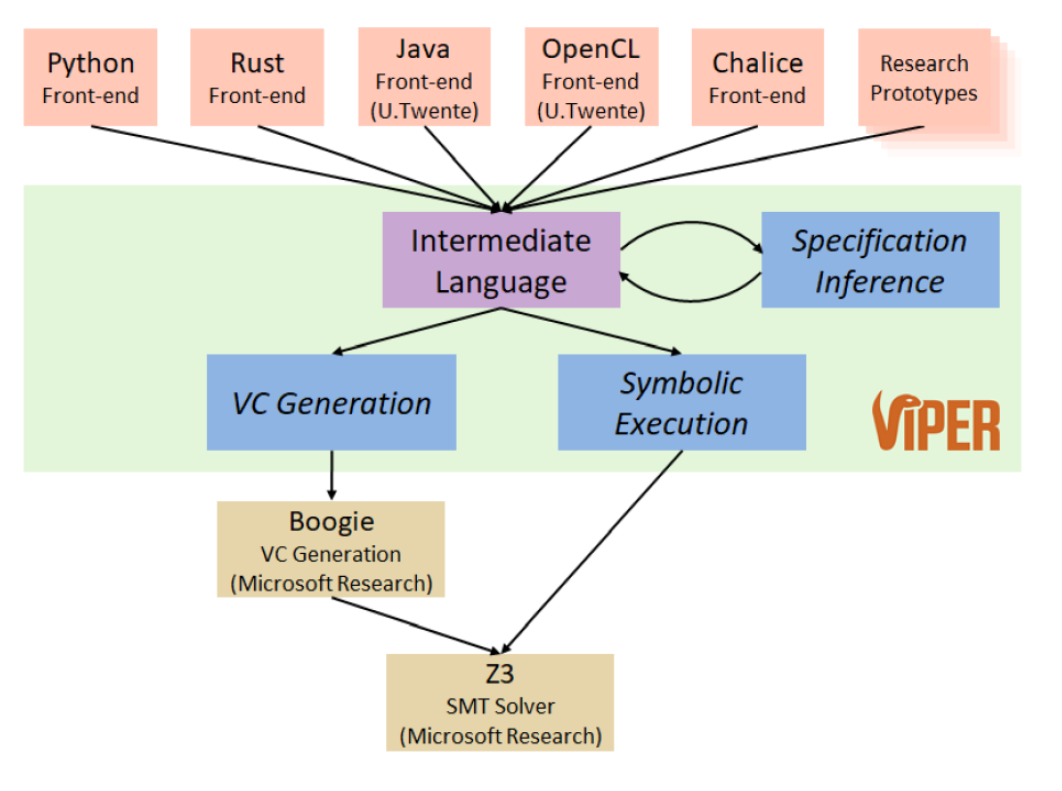
\includegraphics[scale=0.50]{content/images/static-analysis/viper.png}
\end{frame}

\subsection{Frama-C and WP}
\begin{frame}{Why Frama-C?}
\begin{itemize}	
\item "Software is hard." Donald Knuth.
\item "C is quirky, flawed, and an enormous success" Denis  Ritchie.
\item " [C has] the power of assembly language and the convenience of … assembly language. " Denis Ritchie 
\item "For infrastructure technology, C will be hard to displace". Denis  Ritchie
\item The C language is old (1972)
\item The C language is complicated (ISO C 99 = 550 pages)
\item the C language is not perfect (Undefined Behaviors)
\end{itemize}
\end{frame}


\begin{frame}{Why Frama-C ?}
\begin{itemize}	
	\item Developed since 2004 by CEA LIST and INRIA.
	\item Supports code analysis with regard to the ISO C 99.
	\item Uses a formal language ACSL for:
	\begin{itemize}
		\item writing formal specification.
		\item analyzing annotated C programs with ACSL.
	\end{itemize}
    \item Plugin architecture:
    \begin{itemize}
    	\item Kernel: generic Functions: preliminary analysis, pretty printing ...
    	\item Plug-ins: code transformers or analyzers.
    \end{itemize}
\end{itemize}
\end{frame}

\begin{frame}{Frama-C: WP Plugin}
\centering 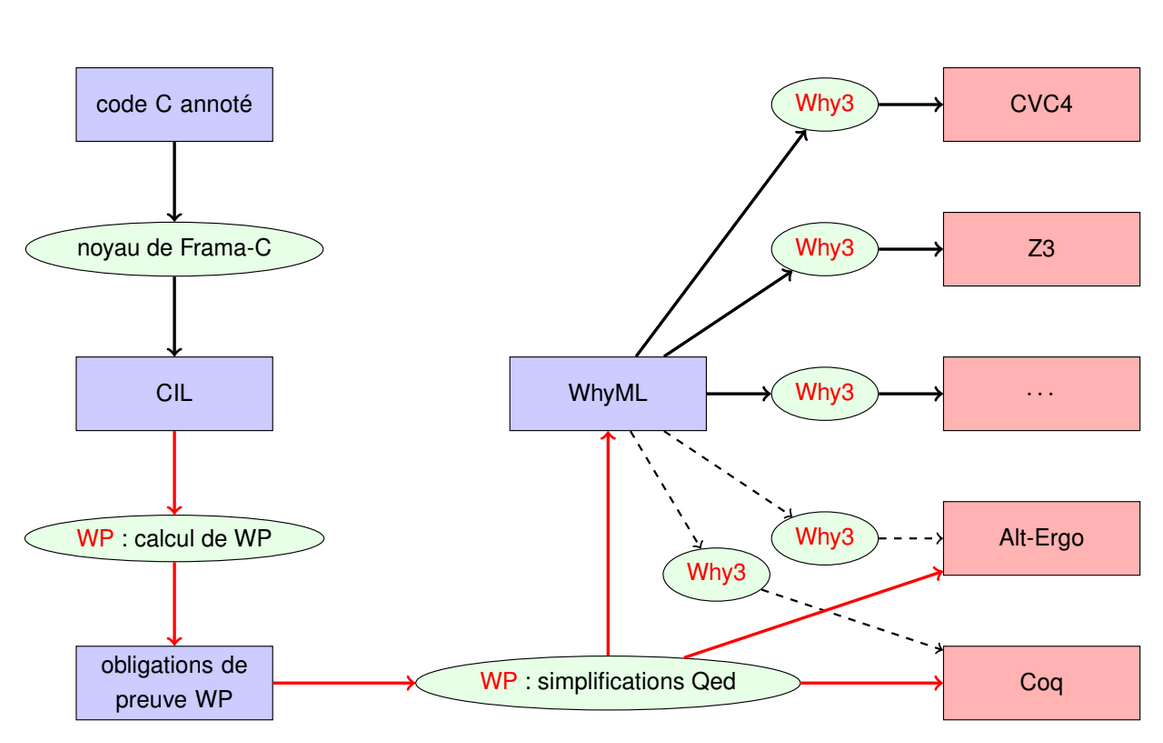
\includegraphics[scale=0.50]{content/images/static-analysis/wp.PNG}
\end{frame}

\begin{frame}{Frama-C: WP Plugin Usage}
\begin{itemize}
	\item Avionic Systems:
	\begin{itemize}
		\item Programs for the A380, A350 and A400M
		\item Replacing unitary testing by unitary deductive proofs.
		\item Argument to qualify for the Certification DO178 B/C, Level A.
	\end{itemize}
\item SCADA SYSTEMS (Supervisory Control of Data Acquisition)
\begin{itemize}
	\item Verification of Temporal properties
	\item 100 000 + lines of code
	\item Qualification for the IEC60880, Class 1
	\item Was Combined with Abstract interpretation.
\end{itemize}
\end{itemize}
\end{frame}

\begin{frame}{ACSL}
\begin{itemize}
	\item \textcolor{blue}{ACSL} was designed to write formal specification tailored to C.
	\item Similar languages:
	\begin{itemize}
		\item  \textcolor{blue}{JML} for Java
	    \item  \textcolor{blue}{Spec\#} for C\#
	    \item  \textcolor{blue}{Spark2014} for Java
	\end{itemize}
\item Build upon the idea of program contracts coming from Eiffel.
\item annotations are added in C code as follow:\\
\textcolor{red}{/*@ ... */} or \textcolor{red}{//@ ... }
\item \textcolor{red}{//@ ensures $\backslash$result == x;}\\
int identity (int x) \{return x;\}
\end{itemize}
\end{frame}

\begin{frame}{ACSL: typing}
\begin{itemize}
	\item ACSL supports mathematical types
	\begin{itemize}
		\item  \textcolor{blue}{integer} for $\mathbb{Z}$
		\item  \textcolor{blue}{real} for $\mathbb{R}$
	\end{itemize}
	\item ACSL supports machine types
\begin{itemize}
	\item  \textcolor{blue}{int} subtype of \textcolor{blue}{integer} 
	\item  \textcolor{blue}{float}, \textcolor{blue}{double} subtypes of \textcolor{blue}{real}
\end{itemize}
\item Problem with \textbf{Runtime-Errors}, combine wp plugin with other plugins to add preconditions to avoid RTE's 
	
\end{itemize}
\end{frame}

\begin{frame}{ACSL: Pre-condition and Post-condition}
\begin{itemize}
	\item The language key words all starts with "$\backslash$"
	\item Post-conditions:
	\begin{itemize}
		\item \textcolor{blue}{ensures $\backslash$result == x;}
		\item \textcolor{blue}{assigns x or $\backslash$nothing }
	\end{itemize}
       \item Pre-condition: \textcolor{blue}{requires x >= t;}

\item terms
\begin{itemize}
	\item C expression such as x - a
	\item keyword: \textcolor{blue}{$\backslash$result, $\backslash$nothing, ...}
	\item predifined logical functions: \textcolor{blue}{$\backslash$sqrt, ...}

\end{itemize}
\item Predicates:
\begin{itemize}
	\item Comparison: \textcolor{blue}{$==, <= , <, != ...$}
	\item Logical connectors: \textcolor{blue}{\&\&$, || , ==>, <==> ...$}
   \item Quantification: \textcolor{blue}{$\backslash forall~~ integer~ x,y; \backslash exists~~integer~z;~ x+y==z$}
   \item Predifined predicates: \textcolor{blue}{$\backslash valid(p) ...$}
\end{itemize}
\end{itemize}
\end{frame}


\begin{frame}{First contract in WP}
\begin{exampleblock}{post-conditions for  the max function}
Here we have a simple function that computes the maximum of two values, this function does not require precondition:
\lstinputlisting[language=C, basicstyle =\normalsize]{content/images/static-analysis/max.c}
\begin{enumerate}
	\item write a contract saying that the result is greater or equal to x and y. Check it's validity.
	\item add another post-conditions saying the result is eather x or y. check it's validity.
	\item add third post-conditions saying that the program does not modify any value.
\end{enumerate}
\end{exampleblock}
\end{frame}


\begin{frame}{WP fails at runtime errors}
Here we have a simple function computing the absolute value of an int:
\lstinputlisting[language=C, basicstyle =\normalsize]{content/images/static-analysis/abs.c}
\begin{enumerate}
	\item write a contract saying that if x is positive than the result is x and if x is strictly negative then the result is -x .
	\item check the contract by options -wp.
	\item check the program using eva.
	\pause
	\item int x means that $-2147483648\leq x \leq 2147483647$
	\item Add a precondition to avoid this issue.
	
\end{enumerate}
\end{frame}
\begin{frame} {Behavioral annotation}
We can describe a program's contract using Behaviors:\\
\textcolor{blue}{/*@ requires R;}   (Global pre-condition)\\
\textcolor{blue}{    behavior b1 :}      (A behavior) \\
\textcolor{blue}{assumes A1; }      ( a guard characterizing the behavior)\\
\textcolor{blue}{requires R1; }     (local pre-condition )\\
\textcolor{blue}{ensures E1;  }     (local post-condition)\\
\textcolor{blue}{assigns L1; }      (values assignes during b1)\\
...               \\
behavior bn:    \\
assumes An;    \\
requires Rn;   \\
ensures En;    \\
assigns Ln;     \\

\textcolor{blue}{complete behaviors; }   ($\bigsqcup b_i = Program~ behavior$ )\\ 
\textcolor{blue}{disjoint behaviors; */}  ($ i\neq j \Rightarrow b_i \bigcap b_j =  \emptyset$ ) 
\end{frame}

\begin{frame}{First contract in WP with behaviors}
\begin{exampleblock}{post-conditions for  the max function}
	Here we have a simple function that computes the maximum of two values, this function does not require precondition:
	\lstinputlisting[language=C, basicstyle =\normalsize]{content/images/static-analysis/max.c}
	\begin{enumerate}
		\item Using 2 behaviors, write a contract for the program.
	
	\end{enumerate}
\end{exampleblock}
\end{frame}

\begin{frame}{Modularity of Weakest precondition}
\begin{exampleblock}{Maximum absolute value}
	Here we have a function max\_abs using the two previous functions:
	\lstinputlisting[language=C, basicstyle =\normalsize]{content/images/static-analysis/max_abs.c}
	\begin{enumerate}
		\item copy the body and the contracts of the functions max and abs.
		\item write and check a contract for the function max\_abs.
		
	\end{enumerate}
\end{exampleblock}
\end{frame}

\begin{frame}{loops in Frama-c/WP}
\begin{itemize}
	\item In C we also have a for loop.\\
	\textcolor{blue}{for(i=0; i<n ;i++);}
    \item for WP/frama-c, we nood to specify 3 predicates for loops (while/for):
    
    	 \textcolor{blue}{loop invariant $0 \leq i\leq n;$} Invariant J \\
    	 \textcolor{blue}{loop variant $n-i$;} a loop variant s for the termination\\
    	  \textcolor{blue}{loop assigns i ;} specify the modified values \\
  
\end{itemize}
\end{frame}


\begin{frame}{First loop invariant in Frama-c/WP}
\begin{exampleblock}{Maximum absolute value}
	Here we have a function m:
	\lstinputlisting[language=C, basicstyle =\normalsize]{content/images/static-analysis/m.c}
	\begin{enumerate}
		\item specify and check the program contract as well as the loop predicates.
	\end{enumerate}
\end{exampleblock}
\end{frame}

\begin{frame}{Frama-C/WP wrap up}
\begin{itemize}
	\item Frama-WP is an implementation of the Weakest precondition calculus.
	\item The target language is C, The calculus is able to prove properties during the presence of runtime errors.
	\item The tool requires more than the loop invariant.
	\item More constructs are possible in ACSL/WP.
	\begin{itemize}
		\item ghost variables.
		\item pointer predicates.
		\item axiomatic function specification.
		\item Lemmas ...
	\end{itemize}
\end{itemize}
\end{frame}
\mode<article>
\exercises

\mode
<all>